\chapter{Finite element method: implementation}

\section{Introduction}
In this lecture, we introduce technical ingredients required to implement the finite element method. This lecture is organized as follows:
\begin{itemize}
\item Section~\ref{sec:fe_ref_elem} introduces a few common finite elements defined on reference domains.  Techniques to generate finite elements will be discussed in the section.
\item Section~\ref{sec:fe_phy_elem} introduces physical elements defined on a triangulation $\calT_h$ and comprise the associated approximation space $\calV_h \subset \calV$.  Techniques to map the reference elements to physical elements will be discussed in the section.
\item Section~\ref{sec:fe_quad} introduces the concept of numerical quadrature which we use to perform integrals that appear in bilinear forms and linear forms.
\item Section~\ref{sec:fe_assembly} discusses the assembly of stiffness matrix and load vector using the ingredients discussed in the previous sections.
\item Section~\ref{sec:fe_ess_bc} describes convenient implementation of essential boundary conditions, which are explicitly enforced by the choice of the space.
\item Section~\ref{sec:fe_impl_blas} provides a brief discussion of efficient implementation using BLAS.
\end{itemize}
This is a rather large lecture that covers significant amount of materials. But, by the end of the lecture, we will have all technical ingredients required to implement a finite element solver.

%% Specifically, we introduce ingredients required to compute the stiffness matrix $\hat A_h \in \RR^{n \times n}$ such that
%% \begin{equation*}
%%   \hat A_{h,ij} = a(\phi_j,\phi_i) \quad \forall i,j = 1,\dots,n,
%% \end{equation*}
%% and the load vector $\hat f_h \in \RR^n$ such that
%% \begin{equation*}
%%   \hat f_{h,i} = \ell(\phi_i) \quad \forall i = 1,\dots,n,
%% \end{equation*}
%% where $\{ \phi_i \}_{i=1}^n$ is a basis for the approximation space $\calV_h$ of a dimension $n$.

%% We compute the 
%% The computation of the stiffness matrix and the load vector requires the following ingredients:
%% \begin{enumerate}
%% \item the ability to evaluate function values and gradients for a reference element $\tilde K$.
%% \item the ability to evaluate basis functions values and gradients for a physical element $K \in \calT_h$.
%% \item 
%% \end{enumerate}




%% We need three key ingredients
%% \begin{itemize}
%% \item[1.] a means to evaluate basis function values and gradients at any points in a reference element $\tilde K$.
%% \item[2.] a means to transform the integral over the element $K$ to an integral over the reference element $\tilde K$.
%% \item[3.] a means to approximate the integral over the reference element $\tilde K$ using a quadrature rule.
%% \end{itemize}

%% As we have seen in Lecture~\ref{ch:pos1d}, the computation of a finite element solution requires a few common tasks on the functions in $\calV_h$, such as the evaluation of the function values, the valuation of the gradient values, and the integration of the functions.  Our approach to construct the piecewise polynomial space is to first define a polynomial space on a \emph{reference element} (or a \emph{canonical element}) and then to map the polynomial functions to the actual elements that comprise the triangulation.  

\section{Reference elements}
\label{sec:fe_ref_elem}
\subsection{Reference domains}
We first introduce reference domains on which a reference finite element can be defined. The first reference domain we introduce is the \emph{reference line segment} $\tilde I \subset \RR^1$. (Note that all quantities associated with the reference space bear a tilde ($\tilde \cdot$).)  While the definition of a reference line segment is not universal, our reference line segment, as shown in Figure~\ref{fig:fe_ref_line}, is a unit line segment delineated by two vertices
\begin{equation*}
  \tilde v_1 \equiv 0 \quad \text{and} \quad \tilde v_2 \equiv 1.
\end{equation*}
(In literature, it is just as common to see a reference line segment defined as $(-1,1)$.)  We consider the line segment oriented in the sense that it points from $\tilde v_1$ to $\tilde v_2$.

\begin{figure}
  \centering
  \subfigure[reference line segment $\tilde I$]{
    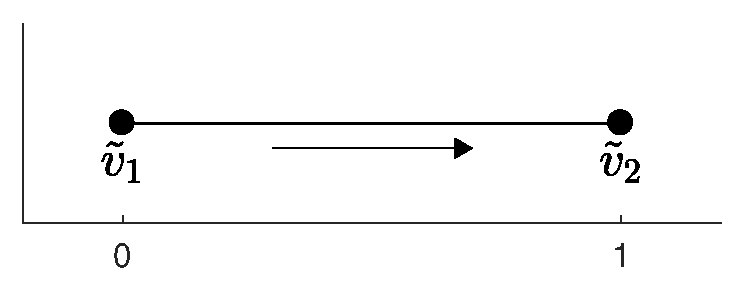
\includegraphics[width=0.3\textwidth]{ref_line}
    \label{fig:fe_ref_line}
  }
  \subfigure[reference triangle $\tilde T$]{
    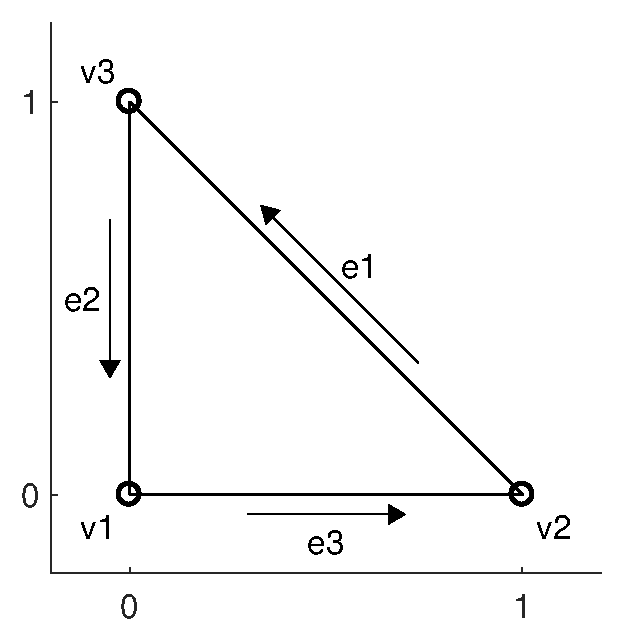
\includegraphics[width=0.3\textwidth]{ref_tri}
    \label{fig:fe_ref_tri}
  }
  \caption{Reference line segment and triangle.\label{fig:fe_ref_elem}}
\end{figure}

  
We next introduce the \emph{reference triangle} $\tilde T \subset \RR^2$. While the definition of a reference triangle is again not universal, our reference triangle, as shown in Figure~\ref{fig:fe_ref_tri}, is a right triangle delineated by three vertices
\begin{equation*}
  \tilde v_1 \equiv (0,0), \quad \tilde v_2 \equiv (1,0), \quad \text{and} \quad \tilde v_3 \equiv (0,1).
\end{equation*}
The vertices are ordered in the counter-clockwise manner, starting with the first vertex at the origin. We also denote the three \emph{facets} of the triangles by
\begin{equation*}
  \tilde F_1 \equiv ( \tilde v_2, \tilde v_3), \quad  \tilde F_2 \equiv ( \tilde v_3, \tilde v_1), \quad \text{and} \quad  \tilde F_3 \equiv ( \tilde v_1, \tilde v_2).
\end{equation*}
(A facet is a $d-1$ entity associated with a canonical shape; for a triangle, a facet is an edge.)  We choose the convention that the facet number is the same as the vertex number of the vertex on the other side of the triangle. Each facet is oriented such that the collection of the three edges defines the triangle in the counter-clockwise orientation.  

We could introduce other reference domains including, for instance, a square in $\RR^2$, a tetrahedron in $\RR^3$, or a cube in $\RR^3$; however, in this lecture, we will only consider the reference line segment $\tilde I$ and the reference triangle $\tilde T$.  

\subsection{Linear Lagrange finite element on a line segment}
\label{sec:fe_lin_line}
We introduce arguably the simplest finite element: linear Lagrange elements on the reference line segment $\tilde I \equiv (0,1) \subset \RR^1$.  To this end, we introduce \emph{Lagrange shape functions} (or \emph{Lagrange basis functions} or \emph{nodal shape functions}) for the space of linear functions on $\tilde I$, $\PP^1(\tilde I)$.
We choose for our interpolation nodes $\{\tilde z_1, \tilde z_2\}$ the endpoints of the line segment:
\begin{equation*}
  \tilde z_1 \equiv 0 \quad \text{and} \quad \tilde z_2 \equiv 1,
\end{equation*}
as shown in Figure~\ref{fig:fe_ref_line_p1}.
  \begin{figure}
    \centering
    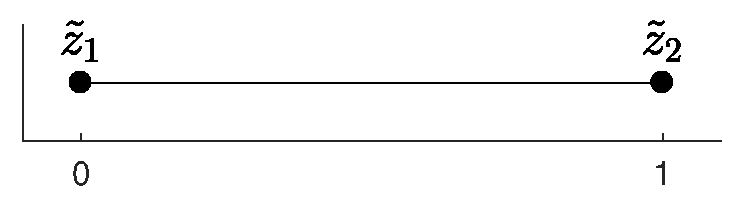
\includegraphics[width=0.3\textwidth]{ref_line_p1}
    \caption{Linear Lagrange finite element on the reference line segment.}
    \label{fig:fe_ref_line_p1}
\end{figure}
Our shape functions are linear functions $\{\tilde \phi_1, \tilde \phi_2\}$ that satisfy the interpolation condition
\begin{equation}
  \tilde \phi_i(z_j) = \delta_{ij}, \quad i,j = 1,2;  \label{eq:fe_line_interp}
\end{equation}
here $\delta_{ij}$ is the \emph{Kronecker delta} such that $\delta_{ij} = 1$ for $i = j$ and $\delta_{ij} = 0$ for $i \neq j$. We readily confirm that the set of two linear function $\{\tilde \phi_1,\tilde \phi_2\}$ that satisfies the interpolation condition~\eqref{eq:fe_line_interp} is a basis for $\PP^1(\tilde I)$.

While the linear Lagrange shape functions can be found by inspection, we here follow a more systematic procedure to construct shape functions that generalizes to higher dimensions and higher-order polynomials. To find the basis, we first express the shape functions in terms of the monomial basis $\{1,\tilde x\}$:
\begin{equation}
  \tilde \phi_j(\tilde x) = c^{(j)}_1 + c^{(j)}_2 \tilde x,  \quad j = 1, 2.
  \label{eq:fe_lin_line_rep}
\end{equation}
We now apply the interpolation condition~\eqref{eq:fe_line_interp} to find the coefficients.  For instance, $\tilde \phi_1$ must satisfy
\begin{equation*}
  \bmat{cc}
  1 & \tilde z_1 \\
  1 & \tilde z_2 \\
  \emat
  \bmat{c}
  c^{(1)}_1 \\ c^{(1)}_2
  \emat
  =
  \bmat{c}
  1 \\ 0 
  \emat
\end{equation*}
We can also pose a single matrix equation for the monomial coefficients of both shape functions: 
\begin{equation*}
  \underbrace{ \bmat{cc}
  1 & \tilde z_1 \\
  1 & \tilde z_2 \\
  \emat }_{V}
  \underbrace{ 
  \bmat{cc}
  c_1^{(1)} & c_1^{(2)} \\
  c_2^{(1)} & c_2^{(2)} \\
  \emat }_{C}
  =
  \bmat{cc}
  1 & 0 \\
  0 & 1 \\
  \emat.
\end{equation*}
We note that the matrix $V$ is the \emph{Vandermonde matrix} associated with our monomial basis $\{ 1,\tilde x\}$ evaluated at the Lagrange interpolation points $\{\tilde z_1, \tilde z_2\}$.  The matrix $V$ is non-singular as long as the interpolation points are distinct, which is the case for our line segment. The unique coefficients are given by
\begin{equation*}
  C
  = V^{-1}
  = \bmat{cc} 1 & 0 \\ 1 & 1 \emat^{-1}
  = \bmat{cc} 1 & 0 \\ -1 & 1 \emat
\end{equation*}
and the associated shape functions are
\begin{align*}
  \tilde \phi_1(\tilde x) &= 1 - \tilde x_1 , \\
  \tilde \phi_2(\tilde x) &= \tilde x_2.
\end{align*}
The shape functions are shown in Figure~\ref{fig:fe_shape_line_p1}.

\begin{figure}
  \centering
  \subfigure[$\tilde \phi_1$]{
    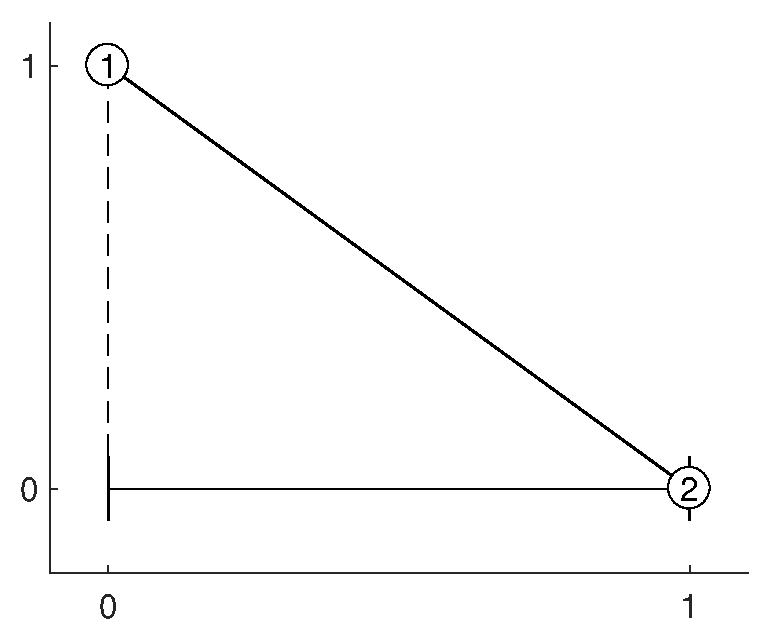
\includegraphics[width=0.3\textwidth]{shape_line_p1_1}
  }
  \subfigure[$\tilde \phi_2$]{
    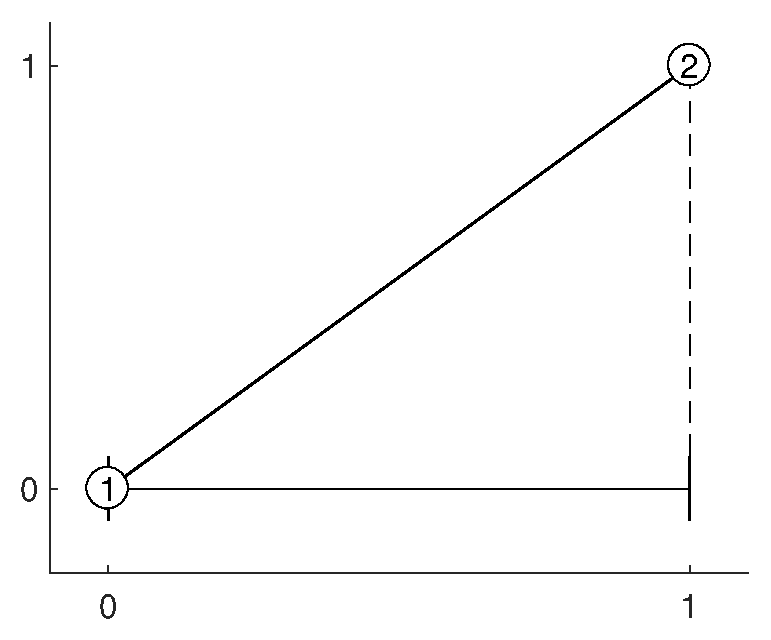
\includegraphics[width=0.3\textwidth]{shape_line_p1_2}
  }
  \caption{Linear Lagrange shape functions on the line segment $\tilde I$. \label{fig:fe_shape_line_p1}}
\end{figure}

Once we find the coefficients of the shape functions, we can evaluate the value of the functions at any point over $\tilde I \subset \RR^1$ by evaluating~\eqref{eq:fe_lin_line_rep}. We can also differentiate~\eqref{eq:fe_lin_line_rep} to obtain the gradient of the shape functions:
\begin{align*}
  \left. \pp{\tilde \phi_i}{\tilde x} \right|_{\tilde x} = c_2^{(i)}.
\end{align*}
More explicitly,
\begin{align*}
  \left. \dd{\tilde \phi_1}{\tilde x} \right|_{\tilde x} = -1
  \quad \text{and} \quad 
  \left. \dd{\tilde \phi_2}{\tilde x} \right|_{\tilde x} = 1.
\end{align*}
The derivatives are constant over the element because the shape functions are linear.

Given the basis $\{\tilde \phi_j\}_{j=1}^2$ for $\PP^1(\tilde I)$, we can uniquely associate any $\tilde v \in \PP^1(\tilde I)$ with a vector $\hat{\tilde v} \in \RR^2$: 
\begin{equation*}
  \tilde v = \sum_{j=1}^2 \hat{\tilde{v}}_j \tilde \phi_j = \sum_{j=1}^2 \tilde v(\tilde z_j) \tilde \phi_j
\end{equation*}
We recognize $\hat{\tilde v} \in \RR^2$ as the \emph{degrees of freedom} with which we can describe functions in $\PP^1(\tilde I)$. For nodal shape functions, $\hat{\tilde v}_j = \tilde v(\tilde z_j)$, $j = 1,2$, due to the Lagrange interpolation condition; the degrees of freedom are the values of the function at the nodes.

Before we introduce other finite elements, we use the linear Lagrange element as an example to describe three properties that formally defines a \emph{finite element}:
\begin{enumerate}
\item the domain over which the element is defined; e.g., the reference line segment $\tilde I$.
\item the finite-dimensional linear space of functions; e.g., the linear polynomial space $\PP^1(\tilde I)$.
\item the degrees of freedom used to describe functions; e.g., for $\tilde v \in \PP^1(\tilde I)$, the degrees of freedom are the values at the nodes $\{ \tilde v(\tilde z_1), \tilde v(\tilde z_2) \}$.
\end{enumerate}



\subsection{Linear Lagrange finite element on a triangle}
\label{sec:fe_lin_tri}

We next introduce a linear Lagrange element on the reference triangle $\tilde T \subset \RR^2$.  Linear functions in $\RR^2$ takes on the form $a_1 + a_2 \tilde x_1 + a_3 \tilde x_2$ and has three degrees of freedom; we hence need to identify a linear independent set of three linear functions.  In our case, we wish to identify a set of three linear \emph{Lagrange basis functions} for the space.  We choose for our interpolation nodes the three vertices of the triangle
\begin{equation*}
  \tilde z_1 \equiv (0,0),
  \quad \tilde z_2 = (1,0),
  \quad \text{and} \quad \tilde z_3 = (0,1),
\end{equation*}
as shown in Figure~\ref{fig:fe_ref_tri_p1}. Our shape functions are linear functions $\{ \tilde \phi_1, \tilde \phi_2, \tilde \phi_3 \}$ that satisfy the interpolation condition
\begin{equation}
  \tilde \phi_i(\tilde z_j) = \delta_{ij} \quad i,j = 1,\dots,3,
   \label{eq:fe_interp_tri}
\end{equation}
where $\delta_{ij}$ is the Kronecker delta.

\begin{figure}
  \centering
  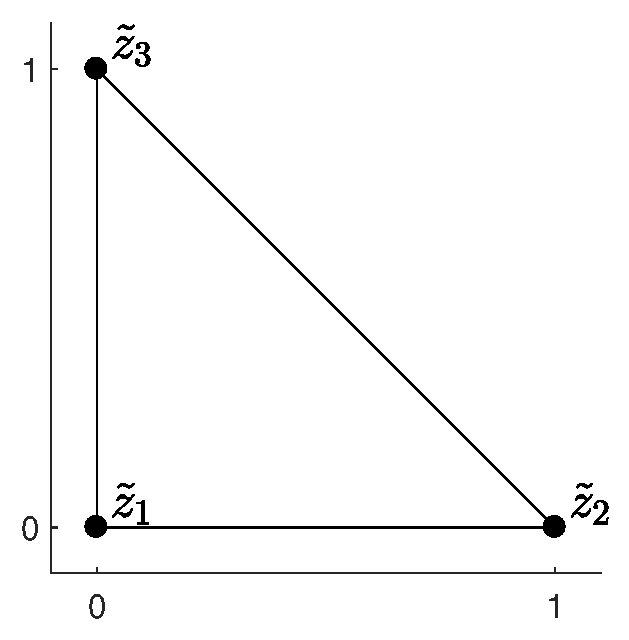
\includegraphics[width=0.3\textwidth]{ref_tri_p1}
  \caption{Linear Lagrange finite element on the reference triangle.}
  \label{fig:fe_ref_tri_p1}
\end{figure}

We identify the shape functions using the same procedure used to identify the linear Lagrange shape functions on the unit line segment in Section~\ref{sec:fe_lin_line}. We first express the shape functions in terms of the monomial basis $\{ 1, \tilde x_1, \tilde x_2 \}$:
\begin{equation}
  \tilde \phi_j(\tilde x) = c^{(j)}_1 + c^{(j)}_2 \tilde x_1 + c_3^{(j)} \tilde x_2 \quad j = 1, 2, 3.
  \label{eq:fe_lin_tri_rep}
\end{equation}
We then apply the interpolation condition~\eqref{eq:fe_interp_tri} to find the coefficients: 
\begin{equation*}
  \underbrace{
   \bmat{ccc}
  1 & \tilde z_{1,1} & \tilde z_{1,2} \\
  1 & \tilde z_{2,1} & \tilde z_{2,2} \\
  1 & \tilde z_{3,1} & \tilde z_{3,2} \\
  \emat }_{\equiv V}
  \underbrace{ 
  \bmat{ccc}
  c_1^{(1)} & c_1^{(2)} & c_1^{(3)} \\
  c_2^{(1)} & c_2^{(2)} & c_2^{(3)} \\
  c_3^{(1)} & c_3^{(2)} & c_3^{(3)} \\
  \emat
  }_{\equiv C}
  =
  \bmat{ccc}
  1 & 0 & 0 \\
  0 & 1 & 0 \\
  0 & 0 & 1
  \emat,
\end{equation*}
where $\tilde z_{i,j}$ is the $j$-th coordinate of the $i$-th interpolation node. The Vandermonde matrix $V$ is non-singular as long as the interpolation points are not collinear, which is equivalent to the condition that the triangle have a finite area; the condition is obviously satisfied for our reference triangle $\tilde T$. The coefficients are given by 
\begin{equation*}
  C = V^{-1}
  = \bmat{ccc}
  1 & 0 & 0 \\
  1 & 1 & 0 \\
  1 & 0 & 1 
  \emat^{-1}
  = \bmat{ccc}
  1 & 0 & 0\\
  -1 & 1 & 0 \\
  -1 & 0 & 1
  \emat;
\end{equation*}
the associated shape functions are
\begin{align}
  \tilde \phi_1(\tilde x) &= 1 - \tilde x_1 - \tilde x_2 \notag \\
  \tilde \phi_2(\tilde x) &= \tilde x_1 \label{eq:fe_lin_tri_expl} \\
  \tilde \phi_3(\tilde x) &= \tilde x_2. \notag
\end{align}
Figure~\ref{fig:fe_shape_tri_p1} visualizes the three basis functions.

\begin{figure}
  \centering
  \subfigure[$\tilde \phi_1$]{
    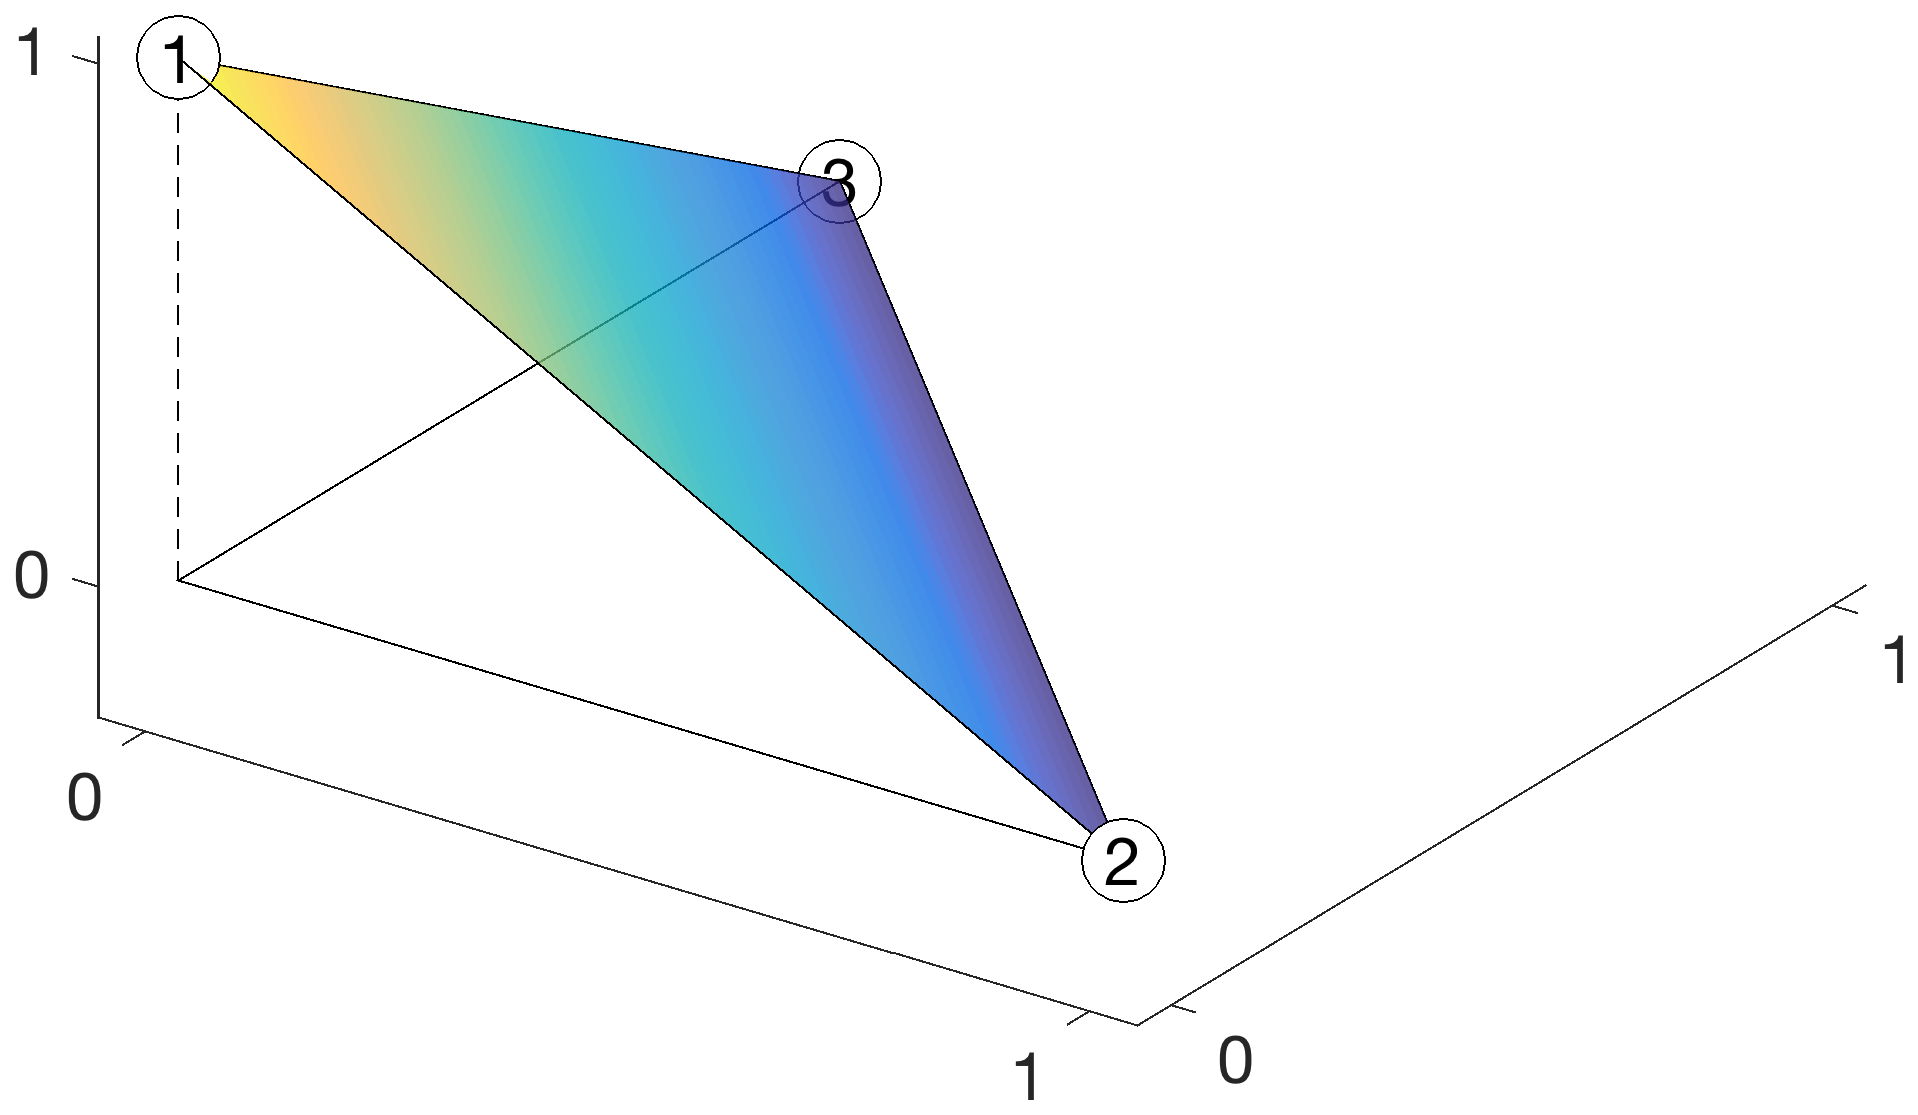
\includegraphics[width=0.3\textwidth]{shape_tri_p1_1}
  }
  \subfigure[$\tilde \phi_2$]{
    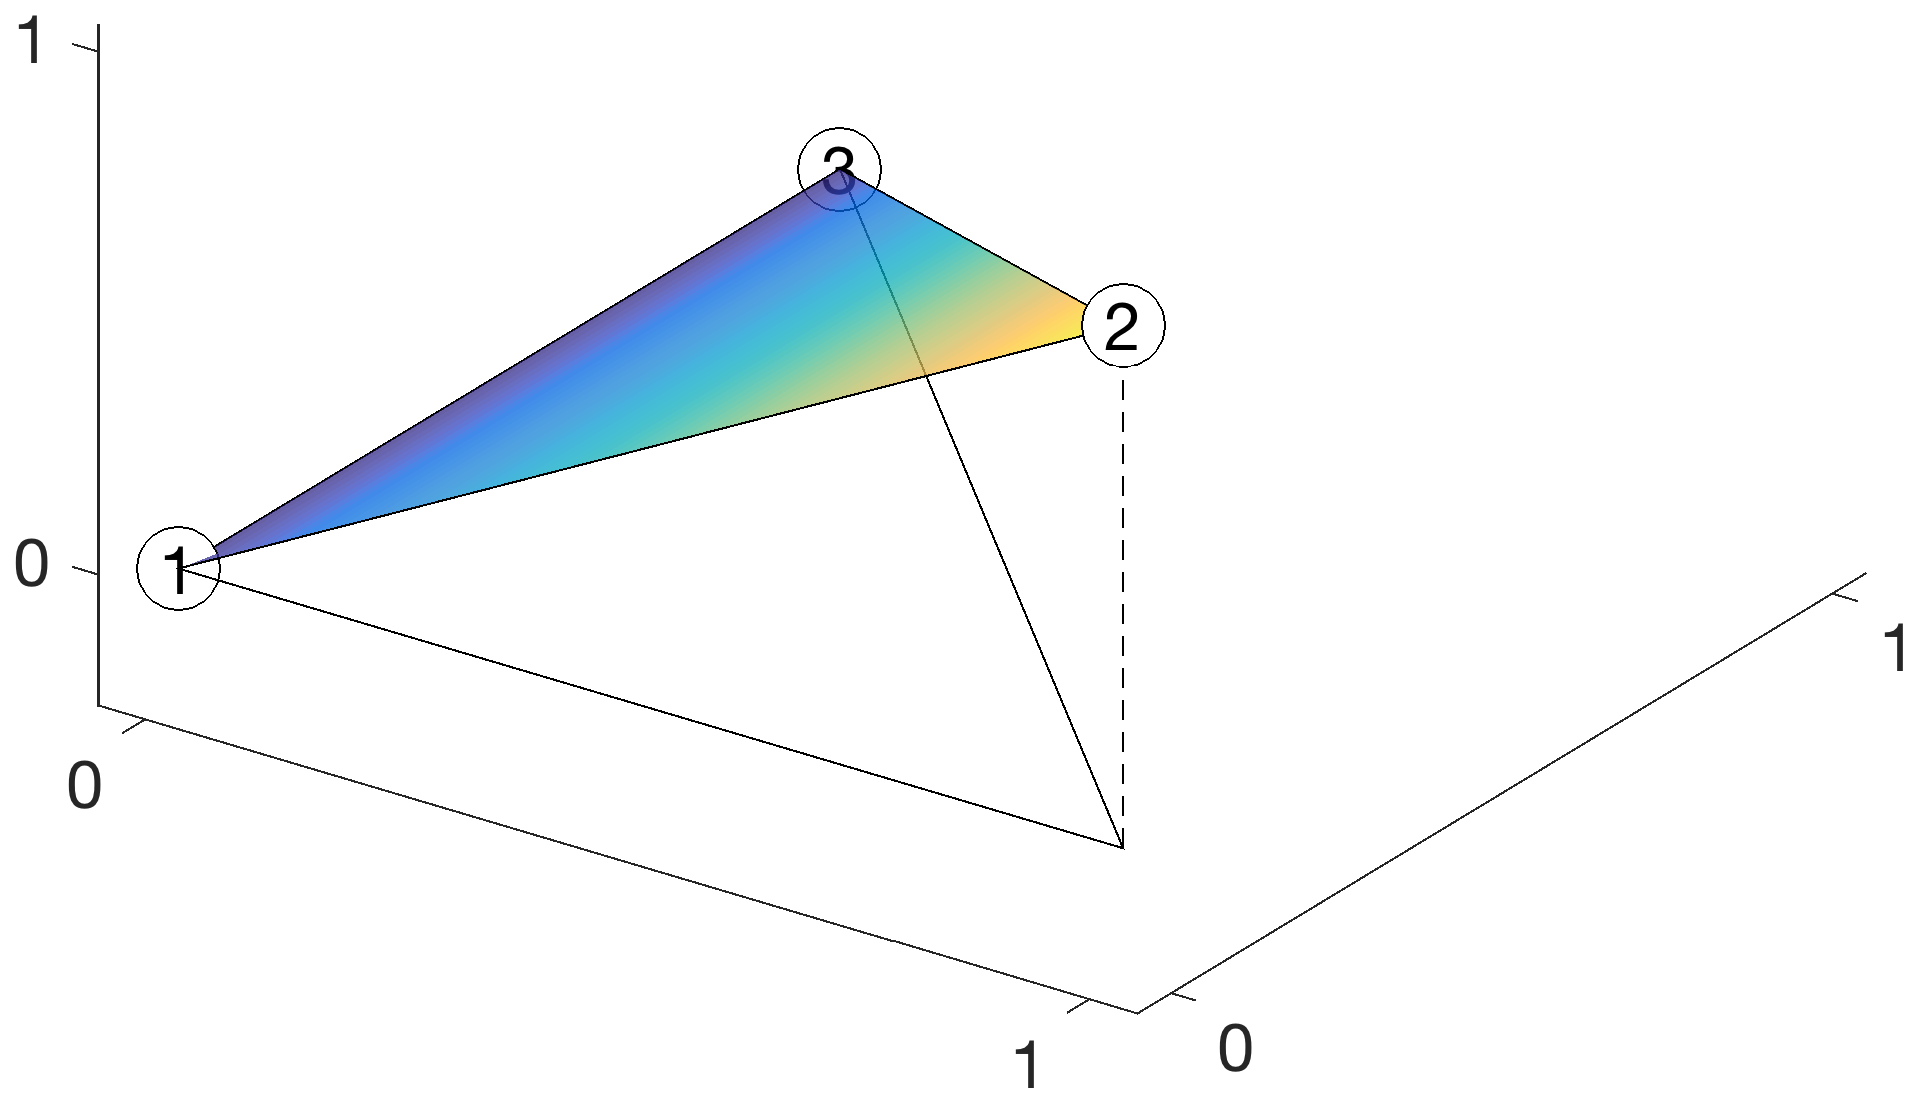
\includegraphics[width=0.3\textwidth]{shape_tri_p1_2}
  }
  \subfigure[$\tilde \phi_3$]{
    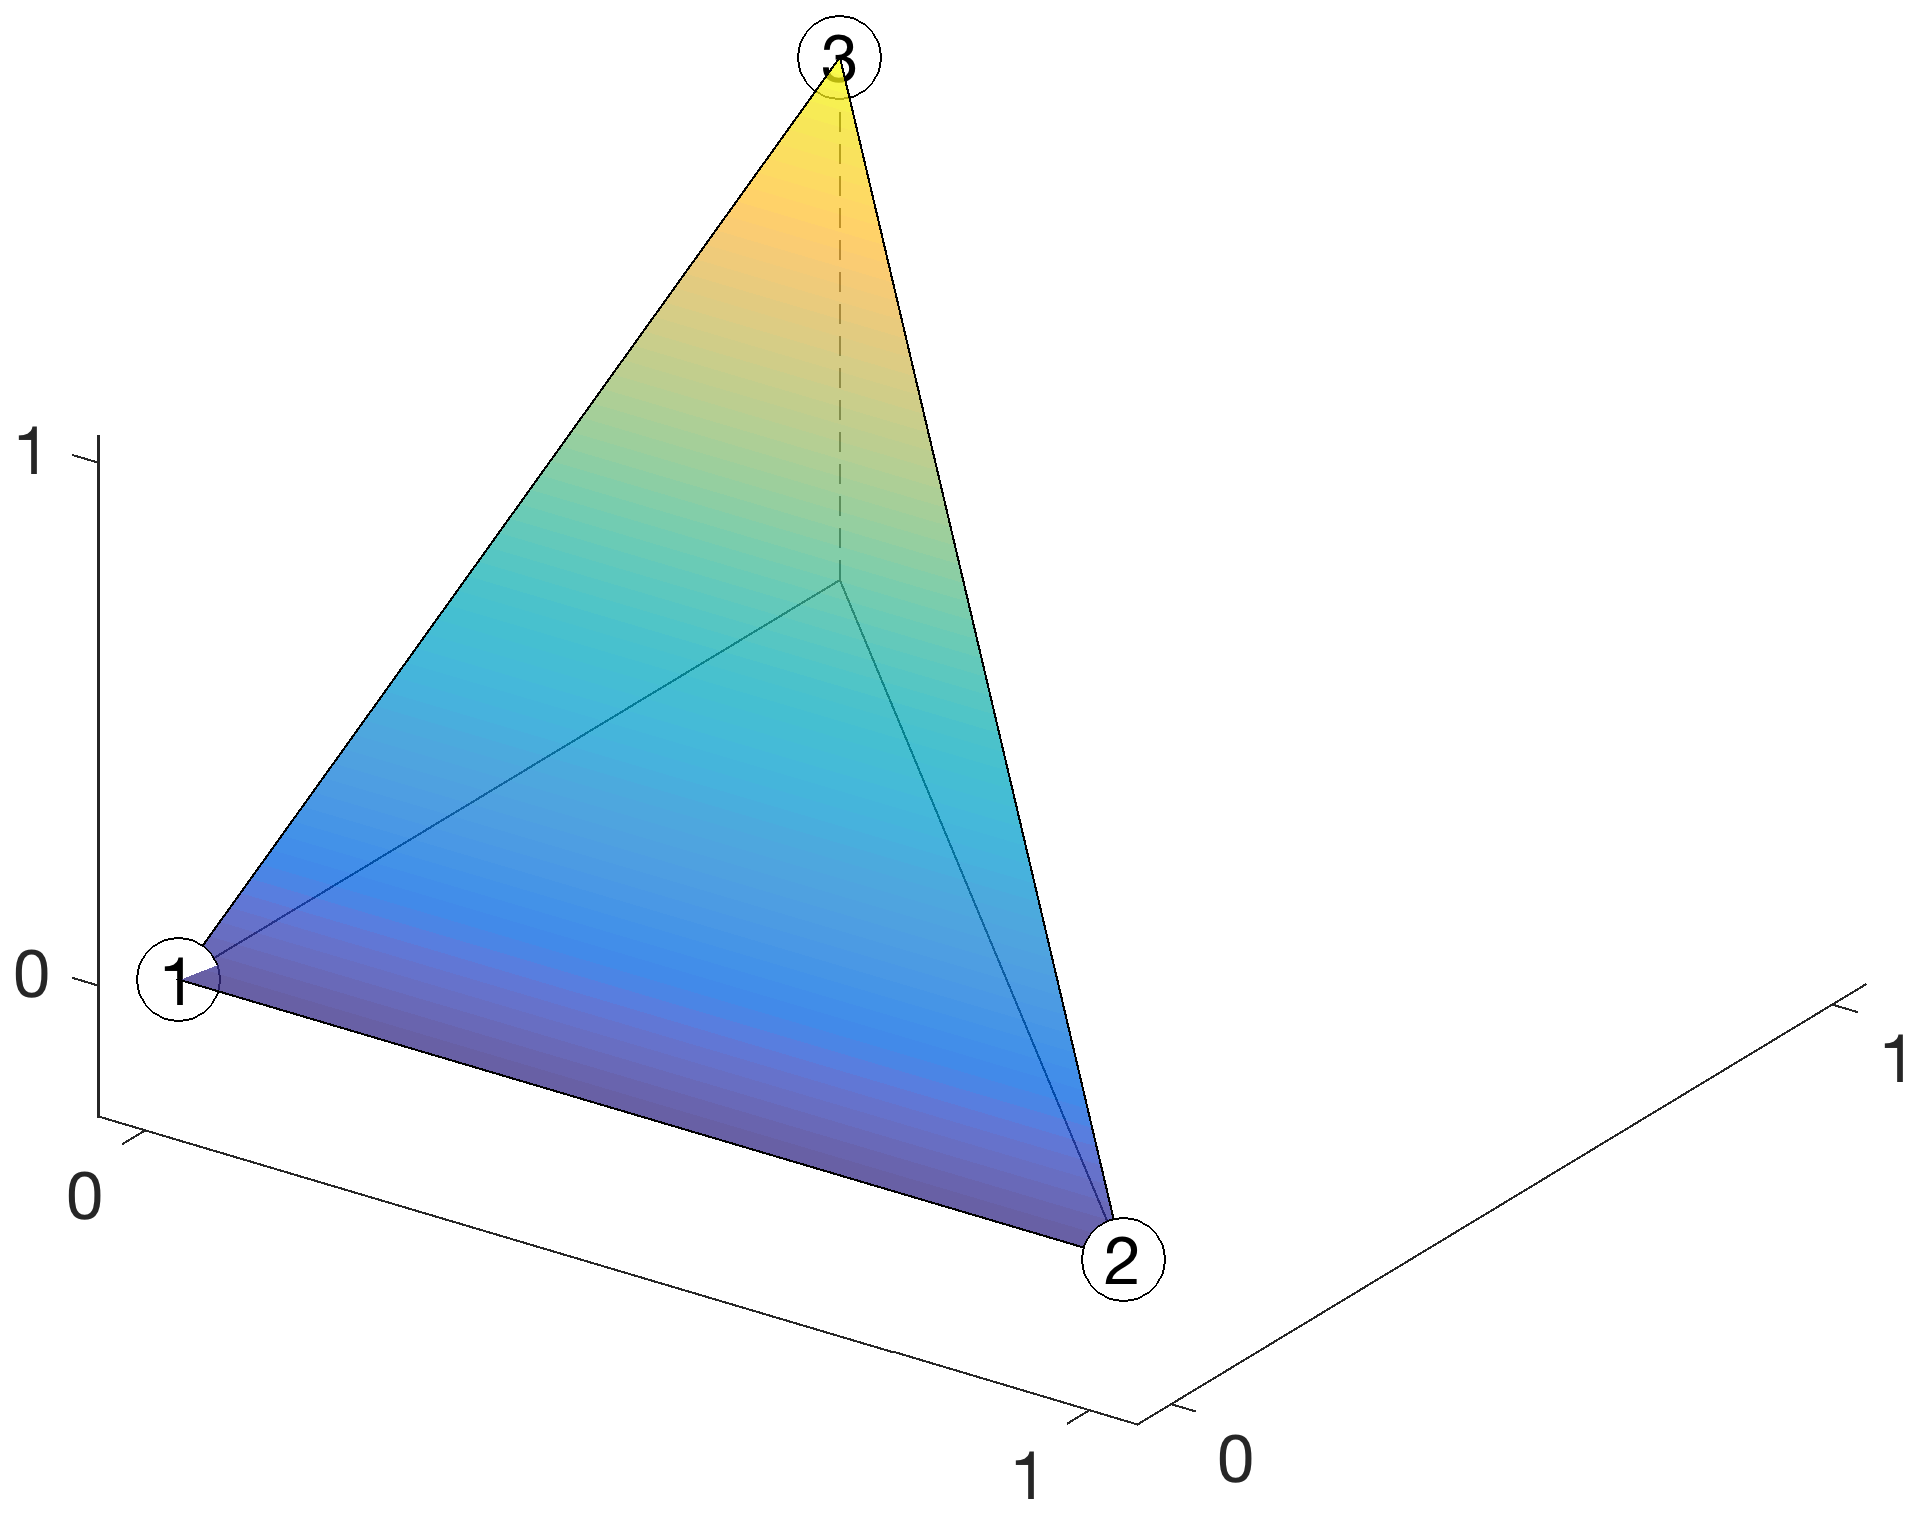
\includegraphics[width=0.3\textwidth]{shape_tri_p1_3}
  }
  \caption{Linear Lagrange shape functions on the reference triangle $\tilde K$.}
  \label{fig:fe_shape_tri_p1}
\end{figure}
We can also differentiate~\eqref{eq:fe_lin_tri_rep} to obtain the gradient of the shape functions:
\begin{equation*}
  \left. \pp{\tilde \phi_j}{\tilde x_1} \right|_{\tilde x} = c_2^{(j)} \quad \text{and} \quad  \left. \pp{\tilde \phi_j}{\tilde x_2} \right|_{\tilde x} = c_3^{(j)}, \quad j = 1,2,3.
\end{equation*}
More explicitly,
\begin{align*}
  \left. \pp{\tilde \phi_1}{\tilde x_1} \right|_{\tilde x} = -1
  \quad &\text{and} \quad
  \left. \pp{\tilde \phi_1}{\tilde x_2} \right|_{\tilde x} = -1\\
  \left. \pp{\tilde \phi_2}{\tilde x_1} \right|_{\tilde x} = 1
  \quad &\text{and} \quad
  \left. \pp{\tilde \phi_2}{\tilde x_2} \right|_{\tilde x} = 0\\
  \left. \pp{\tilde \phi_3}{\tilde x_1} \right|_{\tilde x} = 0
  \quad &\text{and} \quad
  \left. \pp{\tilde \phi_3}{\tilde x_2} \right|_{\tilde x} = 1.
\end{align*}
For the linear Lagrange element, the derivatives are constant (and trivially spans $\PP^0(\tilde T)$).

Given the basis $\{ \tilde \phi_j \}_{j=1}^3$, we can uniquely associate any function $\tilde v \in \PP^1(\tilde T)$ with a vector $\hat{\tilde v} \in \RR^3$:
\begin{equation*}
  \tilde v = \sum_{j=1}^3 \hat{\tilde v}_j \tilde \phi_j = \sum_{j=1}^3 \tilde v(\tilde z_j) \tilde \phi_j.
\end{equation*}
Again, for the nodal shape functions, the degrees of freedom are the values of he functions at the nodes, $\{ \tilde v(\tilde z_j) \}_{j=1}^3$.  To summarize, our linear Lagrange finite element on a triangle is formally defined by (i) the domain --- the reference triangle $\tilde T$ ---, (ii) the linear function space --- the polynomial space $\PP^1(\tilde T)$ ---, and (iii) the degrees of freedom --- the values at the nodes $\{\tilde z_1,\tilde z_2, \tilde z_3\}$.

Before we conclude this section, we introduce a mapping that relates nodes on a facet to nodes on the element. Figure~\ref{fig:fe_ref_tri_face_p1} shows the relationship between the nodes. Our facet-to-node map is 
\begin{equation*}
  \theta_{\tilde F\text{-}n} : \{ 1,2,3 \} \times \{ 1,2 \} \to \{1,2,3\}
\end{equation*}
such that
\begin{align*}
  \theta_{\tilde F\text{-}n}(1,1) &= 2, &   \theta_{\tilde F\text{-}n}(1,2) &= 3, \\
  \theta_{\tilde F\text{-}n}(2,1) &= 3, &   \theta_{\tilde F\text{-}n}(2,2) &= 1, \\
  \theta_{\tilde F\text{-}n}(3,1) &= 1, &   \theta_{\tilde F\text{-}n}(3,2) &= 2.
\end{align*}
Note that $j = \theta_{\tilde F\text{-}n}(i,k)$ is the Lagrange node on $\tilde T$ identified with the $k$-th Lagrange node of the facet $i$; i.e.,
\begin{equation*}
  \tilde z_{j \equiv\theta_{\tilde F\text{-}n}(i,k)}  = \tilde z^{\tilde F_i}_k \quad \forall i =1,2,3, \ k = 1,2.
\end{equation*}
We will make use of the mapping when the bilinear form or the linear form requires integration on a boundary.

%% We now relate the trace of the shape functions on facets $\tilde F_i$, $i = 1,2,3$, to the shape functions on a line segment. To this end, we first note that any restriction of a two-dimensional linear function to a line segment is a linear function on the line segment.  We apply this principle to map the linear shape functions $\{\tilde \phi_j\}_{j=1}^3$ defined on a triangle $\tilde T \subset \RR^2$ to the linear shape functions $\{ \chi_k \}_{k=1}^2$ defined on a line segment $I \subset \RR^1$.

%% The mapping of the Lagrange nodes on the triangle $\tilde T$ to those on the facets $\{ \tilde F_i \}_{i=1}^3$ is shown in Figure~\ref{fig:fe_ref_tri_face_p1}. For instance, the one-dimensional linear shape functions on the facet $\tilde F_1$, $\{ \chi_k^{\tilde F_1} \}_{k=1}^2$, are identified by the Lagrange nodes
%% \begin{equation*}
%%   \tilde z_1^{\tilde F_1} \equiv \tilde z_2 \quad \text{and} \quad
%%   \tilde z_2^{\tilde F_1} \equiv \tilde z_3 ,
%% \end{equation*}
%% and the shape functions are related by
%% \begin{equation*}
%%   \tilde \phi_2 |_{\tilde F_1} = \chi_1^{\tilde F_1}
%%   \quad \text{and} \quad
%%   \tilde \phi_3 |_{\tilde F_1} = \chi_2^{\tilde F_1} .
%% \end{equation*}
%% Analogous relationships exist for the facets $\tilde F_2$ and $\tilde F_3$. 
%% %% Similarly, on the facet $\tilde F_2$, the Lagrange nodes are
%% %% \begin{equation*}
%% %%   \tilde z_1^{\tilde F_2} \equiv \tilde z_3 \quad \text{and} \quad
%% %%   \tilde z_2^{\tilde F_2} \equiv \tilde z_1 ,
%% %% \end{equation*}
%% %% and the shape functions are related by
%% %% \begin{equation*}
%% %%   \tilde \phi_3 |_{\tilde F_2} = \chi_1^{\tilde F_2}
%% %%   \quad \text{and} \quad
%% %%   \tilde \phi_1 |_{\tilde F_2} = \chi_2^{\tilde F_2} ;
%% %% \end{equation*}
%% More compactly, we can introduce a facet-to-element node map
%% \begin{equation*}
%%   \theta_{\tilde F\text{-}n} : \{ 1,2,3 \} \times \{1,2\} \to \{1,2,3\},
%% \end{equation*}
%% such that $j = \theta_{\tilde F\text{-}n}(i,k)$ is the Lagrange node on $\tilde T$ identified with the $k$-th Lagrange node of the facet $i$. In other words,
%% \begin{equation*}
%%   \tilde z_k^{\tilde F_i} \equiv \tilde z_{\theta_{\rm f-e}(i,k)}, \quad k = 1,2, \ i = 1,2,3.
%% \end{equation*}
%% Accordingly, the trace of the two-dimensional shape functions $\{\tilde \phi_j\}_{j=1}^3$ are related to the one-dimensional shape functions by
%% \begin{equation*}
%%   \tilde \phi_{\theta_{\rm f-e}(i,k)}|_{\tilde F_i} = \chi^{\tilde F_i}_k, \quad k = 1,2, \ i = 1,2,3.
%% \end{equation*}
  
\begin{figure}
  \centering
  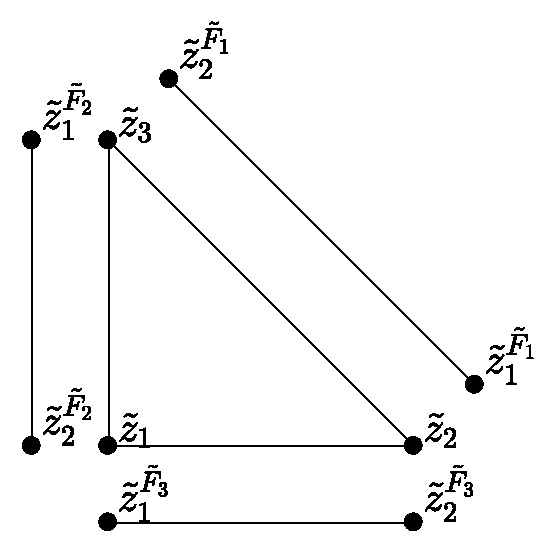
\includegraphics[width=0.35\textwidth]{ref_tri_face_p1}
  \caption{Linear Lagrange triangular element-facet relationship.}
  \label{fig:fe_ref_tri_face_p1}
\end{figure}



\subsection{Quadratic Lagrange finite element on a line segment}
\label{sec:fe_p2_line}
We now introduce a quadratic Lagrange element on the reference line segment $\tilde I \subset \RR^1$. A quadratic function in $\PP^1(\tilde I)$ takes on the form $a_1 + a_2 \tilde x + a_3 \tilde x^2$ and has three degrees of freedom; we hence wish to identify a linearly independent set of three quadratic Lagrange shape functions. To this end, we choose for our Lagrange interpolation nodes the two endpoints and the midpoint,
\begin{equation*}
  \tilde z_1 = 0, \quad \tilde z_2 = 1, \quad \text{and} \quad \tilde z_3 = 1/2. 
\end{equation*}
The ordering of the nodes for a quadratic element is not universal in the finite element literature; we here adhere to the convention that preserves the location of $\tilde z_1$ and $\tilde z_2$ from the linear element.  To find the Lagrange shape functions, we first express the functions in terms of the monomial basis $\{ 1, \tilde x, \tilde x^2 \}$:
\begin{equation}
  \tilde \phi_j(\tilde x) = c_1^{(j)} + c_2^{(j)} \tilde x + c_3^{(j)} \tilde x^2, \quad j = 1,2, 3.
  \label{eq:fe_quad_line_rep}
\end{equation}
We then express the interpolation condition $\tilde \phi_j(\tilde z_i) = \delta_{ij}$ as a $3 \times 3$ system $VC = I$, where $C \in \RR^{3 \times 3}$ is the coefficient matrix so that $C_{ij} = c_i^{(j)}$ and the $i$-th row of the Vandermonde matrix $V \in \RR^{3 \times 3}$ is
\begin{equation*}
  V_{i:} = \bmat{ccc} 1 & \tilde z_i & \tilde z_i^2\emat.
\end{equation*}
The matrix $V$ is non-singular because the monomial basis functions are linearly independent and the three interpolation points are distinct. The shape fucntions are shown in Figure~\ref{fig:fe_shape_line_p2}. 
\begin{figure}
  \centering
  \subfigure[$\tilde \phi_1$]{
    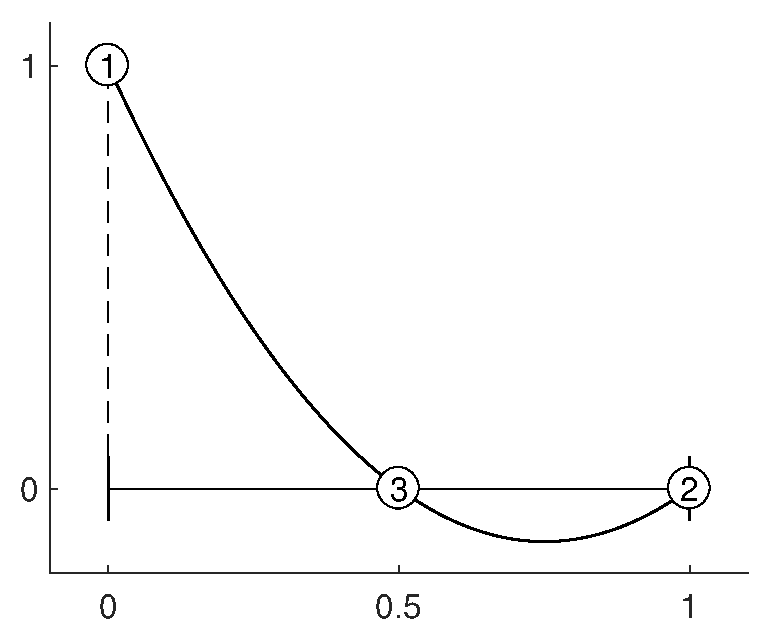
\includegraphics[width=0.3\textwidth]{./shape_line_p2_1}
  }
  \subfigure[$\tilde \phi_2$]{
    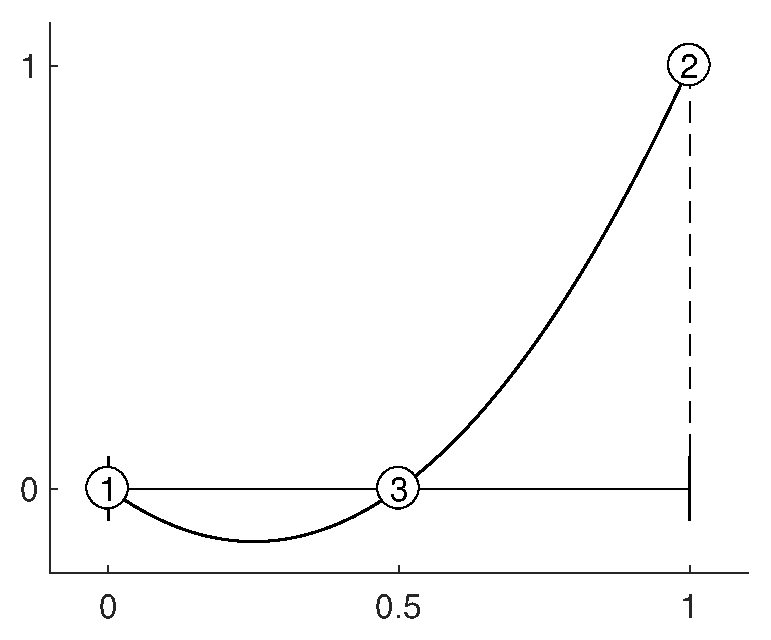
\includegraphics[width=0.3\textwidth]{./shape_line_p2_2}
  }
  \subfigure[$\tilde \phi_3$]{
    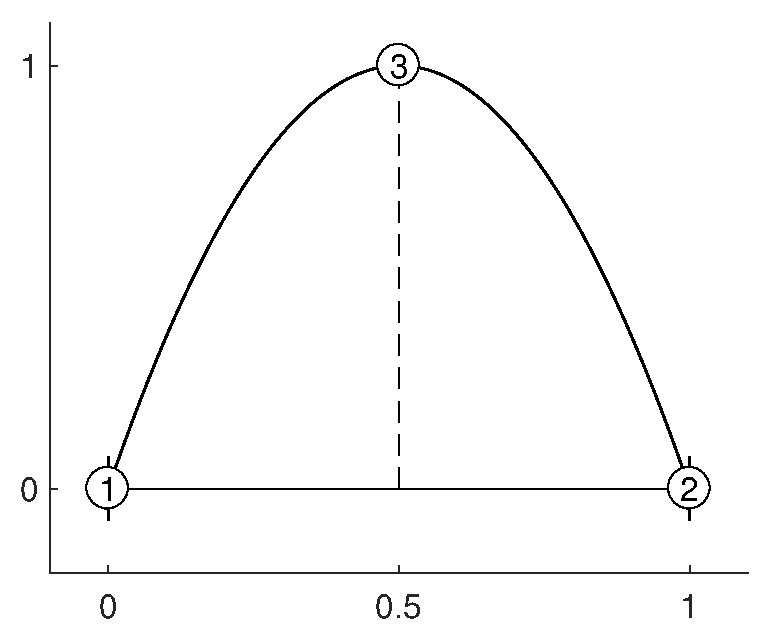
\includegraphics[width=0.3\textwidth]{./shape_line_p2_3}
  }
  \caption{Quadratic Lagrange shape functions on line segment $\tilde I$. \label{fig:fe_shape_line_p2}}
\end{figure}
The differentiation of \ref{eq:fe_quad_line_rep} yields the derivatives of the shape functions:
\begin{equation*}
  \left. \dd{\tilde \phi_j}{\tilde x} \right|_{\tilde x} = c_2^{(j)} + 2 c_3^{(j)} \tilde x , \quad j = 1,2,3.
\end{equation*}
Because the shape functions are quadratic, the derivatives vary linearly over the domain $\tilde I$, and they span $\PP^1(\tilde I)$.  The degrees of freedom for our nodal $\PP^2$ finite element on $\tilde I$ are the values of functions at the three nodes $\{\tilde z\}_{j=1}^3$.

\subsection{Quadratic Lagrange finite element on a triangle}
\label{sec:fe_p2_tri}
We now introduce a quadratic Lagrange finite element on the reference triangle $\tilde T \subset \RR^2$. A quadratic function in $\PP^2(\tilde K)$ takes on the form $a_1 + a_2 \tilde x_1 + a_3 \tilde x_2 + a_4 \tilde x_1^2 + a_5 \tilde x_1 \tilde x_2 + a_6 \tilde x_2^2$ and has six degrees of freedom; we hence wish to identify a linearly independently set of six quadratic Lagrange shape functions.  To this end, we choose for our Lagrange interpolation nodes the three vertices of the triangle and three points at the middle of the edges,
\begin{equation*}
  \tilde z_1 = (0,0), \quad \tilde z_2 = (1,0), \quad \tilde z_3 = (0,1), \quad \tilde z_4 = (1/2,1/2), \quad \tilde z_5 = (0,1/2), \quad \tilde z_6 = (1/2,0),
\end{equation*}
as shown in Figure~\ref{fig:fe_ref_tri_p2}.
\begin{figure}
  \centering
  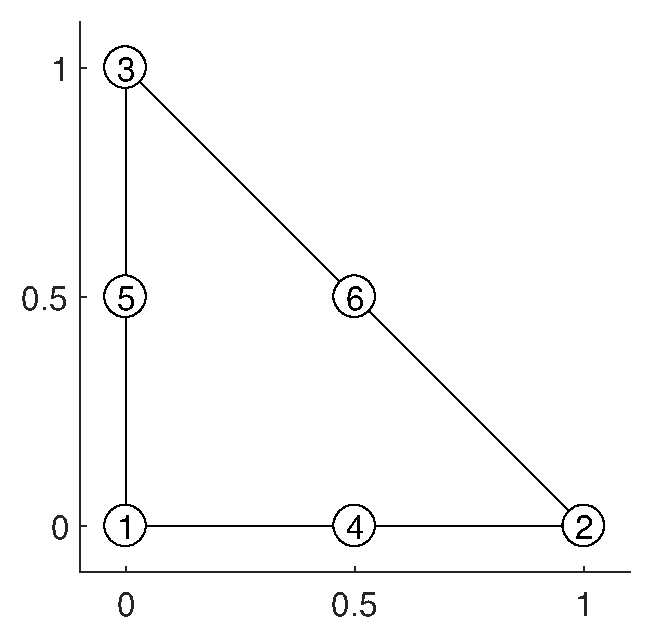
\includegraphics[width=0.3\textwidth]{ref_tri_p2}
  \caption{Quadratic Lagrange finite element on the reference triangle.}
  \label{fig:fe_ref_tri_p2}
\end{figure}
The ordering of the nodes is not universal in the finite element literature; we here adhere to the convention that preserves the location of the $\tilde z_1$, $\tilde z_2$, and $\tilde z_3$ from the linear element and, for $i \in \{4,5,6\}$, the $\tilde z_i$ is on the midpoint of the $(i-3)$-th edge of the reference triangle. To find the Lagrange shape functions, we first express the basis functions in terms of the monomial basis $\{1,\tilde x_1, \tilde x_2, \tilde x_1^2 , \tilde x_1 \tilde x_2, \tilde x_2^2\}$:
\begin{equation}
  \tilde \phi_j(\tilde x) = c_1^{(j)} + c_2^{(j)} \tilde x_1 + c_3^{(j)} \tilde x_2 + c_4^{(j)} \tilde x_1^2 + c_5^{(j)} \tilde x_1 \tilde x_2 + c_6^{(j)} \tilde x_2^2, \quad j = 1,\dots,6.
  \label{eq:fe_quad_tri_rep}
\end{equation}
We then express the interpolation condition $\tilde \phi_j(\tilde z_i) = \delta_{ij}$ as a $6 \times 6$ matrix system $VC = I$, where $C \in \RR^{6 \times 6}$ is the coefficient matrix so that $C_{ij} = c^{(j)}_i$ and the $i$-th row of the Vandermonde matrix $V \in \RR^{6 \times 6}$ is
\begin{equation*}
  V_{i:} = \bmat{cccccc} 1 & \tilde z_{i,1} & \tilde z_{i,2} &  (z_{i,1})^2 & \tilde z_{i,1} \tilde z_{i,2} & (\tilde z_{i,2})^2 \emat .
\end{equation*}
The matrix $V$ is non-singular, and the linear system has a unique solution: $C = V^{-1}$.  Figure~\ref{fig:fe_shape_tri_p2} shows the six basis functions.
\begin{figure}
  \centering
  \subfigure[$\tilde \phi_1$]{
    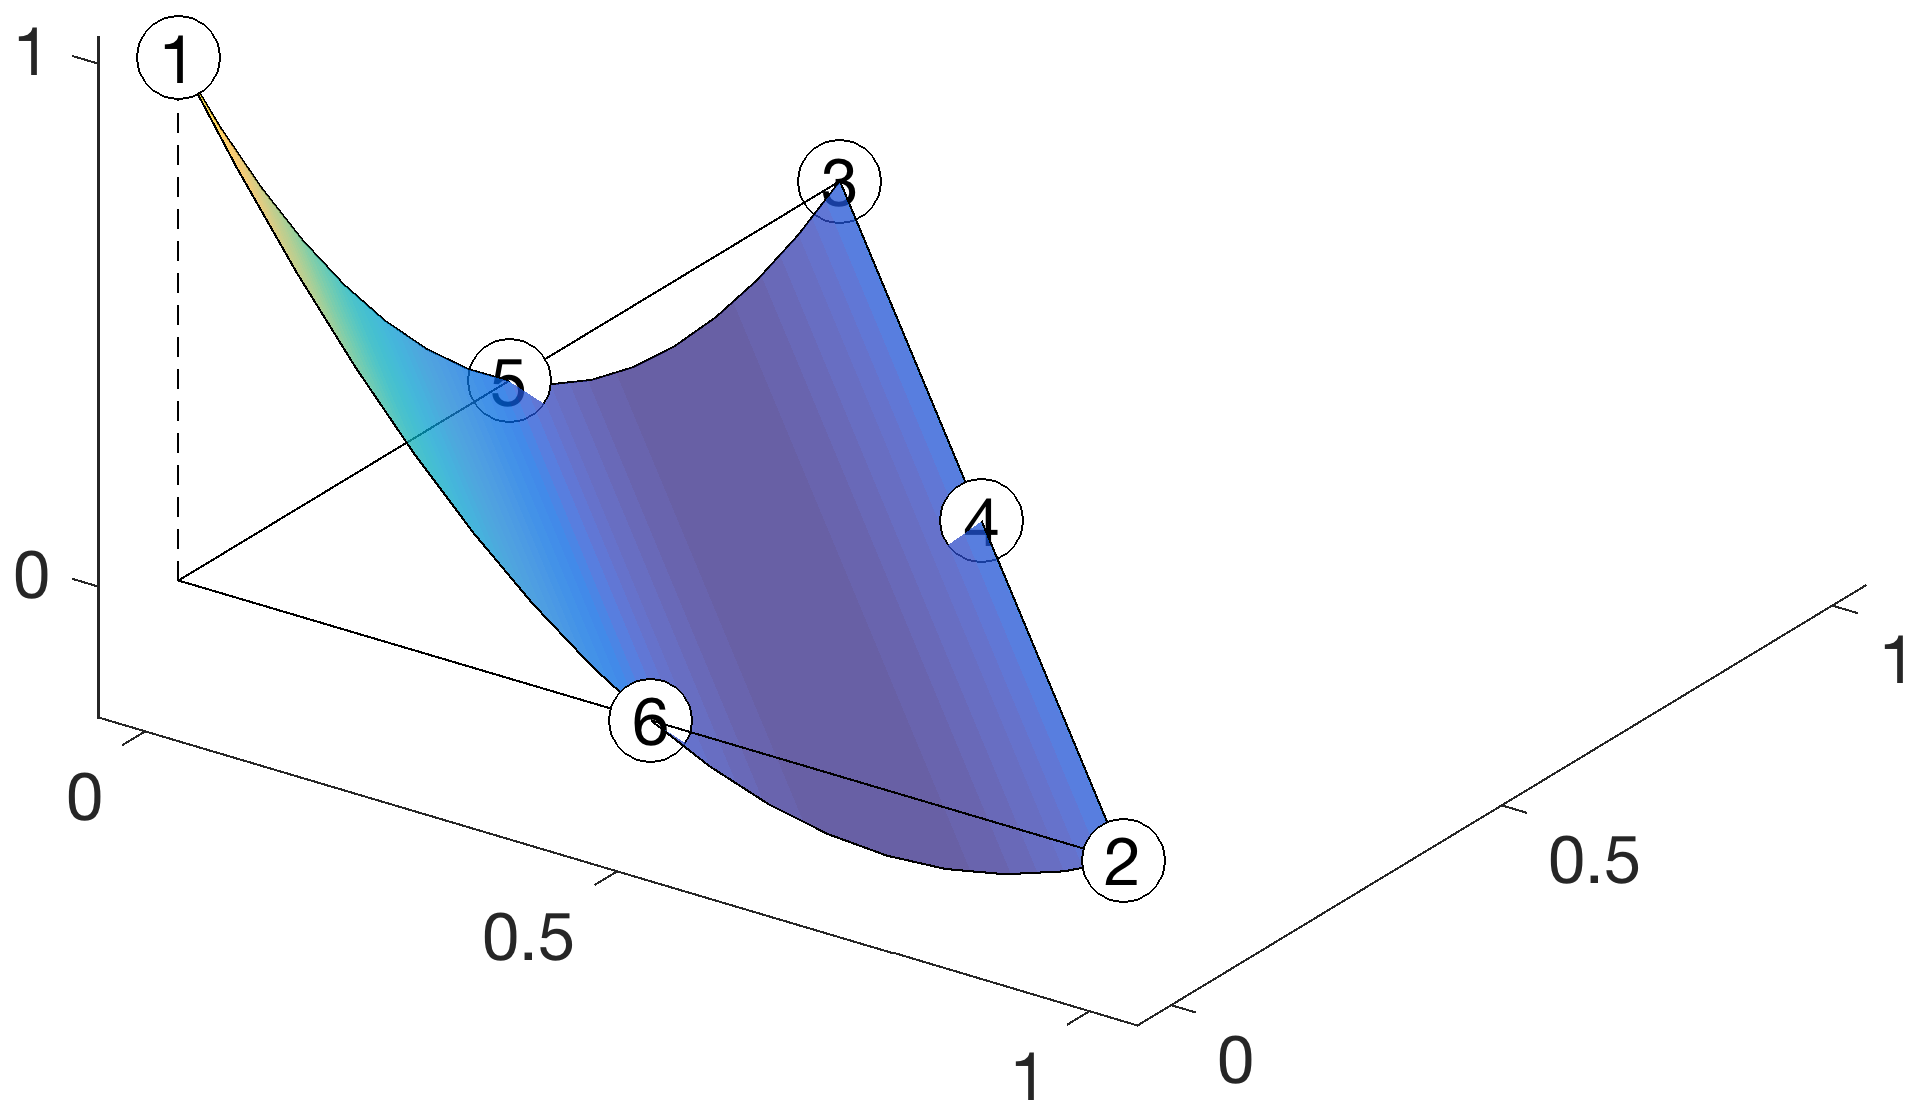
\includegraphics[width=0.3\textwidth]{shape_tri_p2_1}
  }
  \subfigure[$\tilde \phi_2$]{
    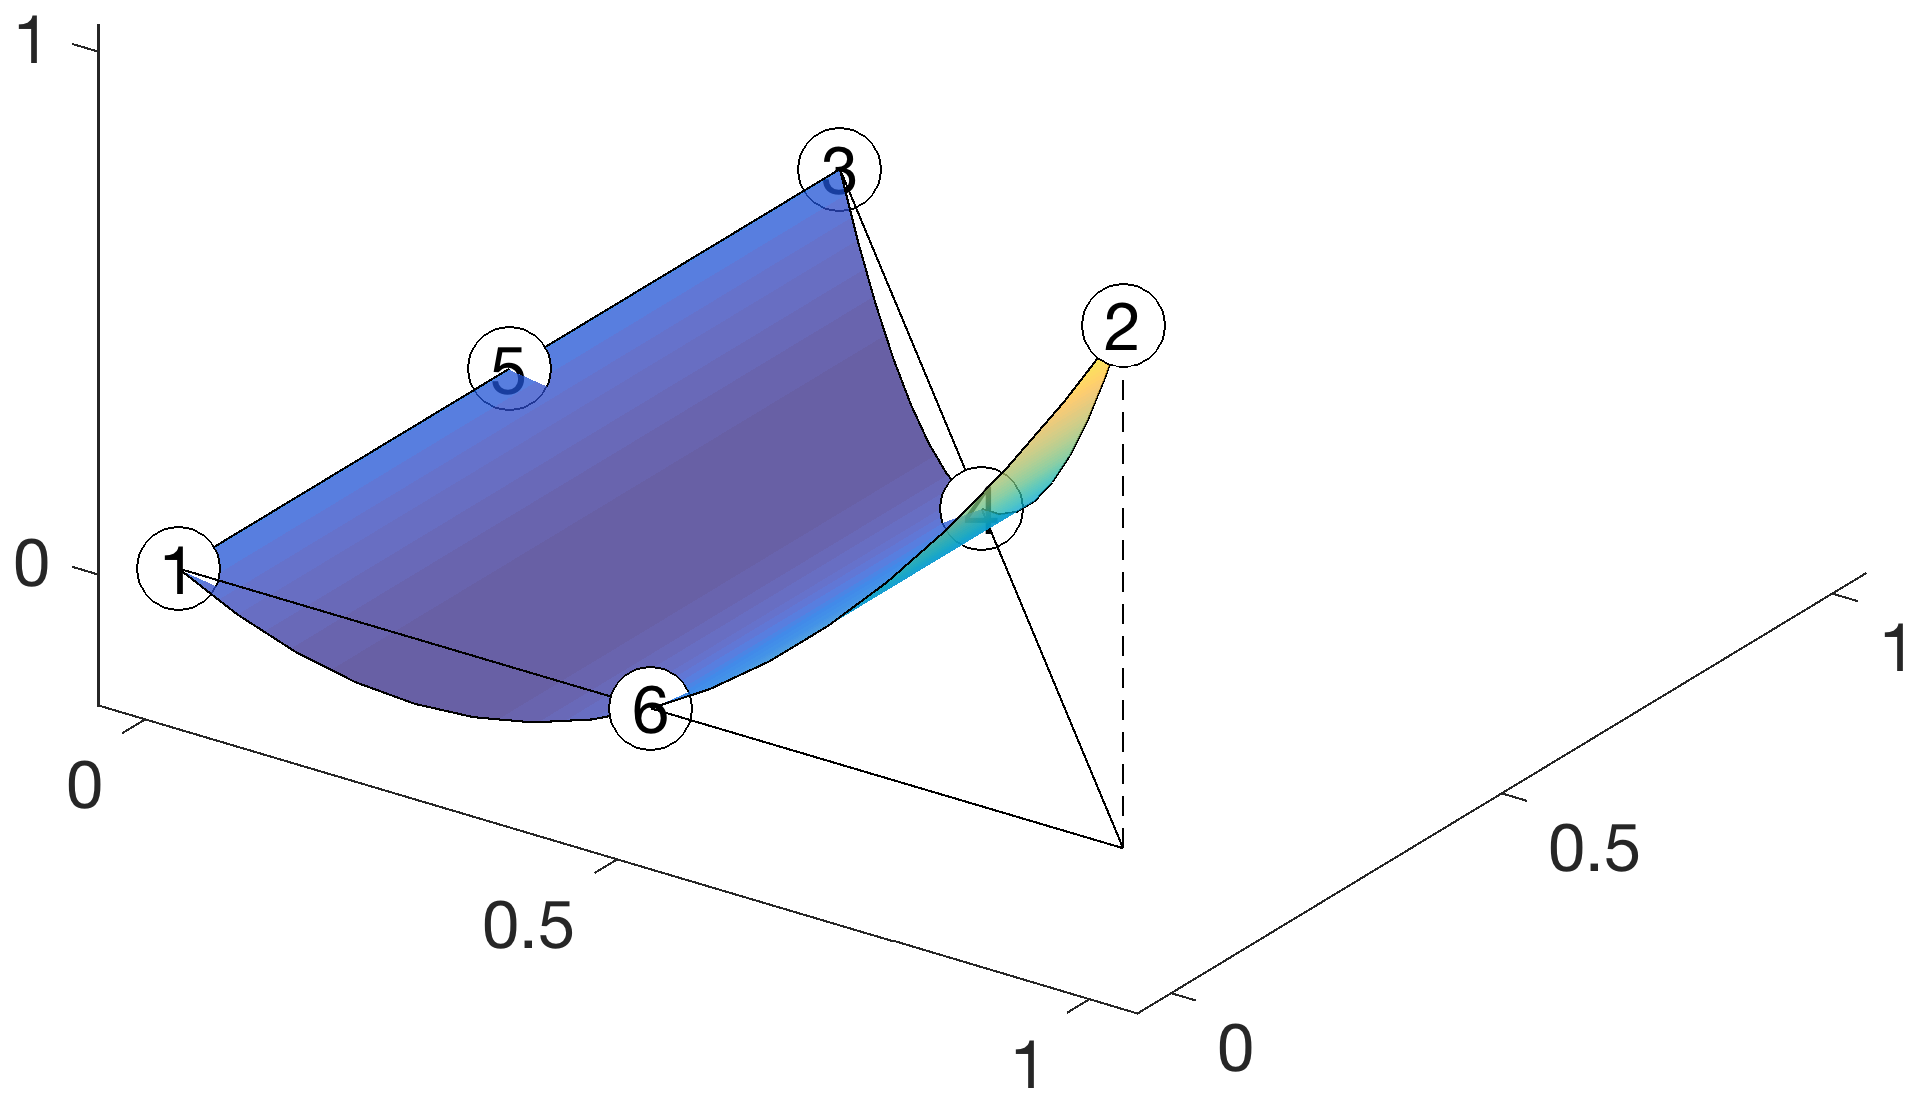
\includegraphics[width=0.3\textwidth]{shape_tri_p2_2}
  }
  \subfigure[$\tilde \phi_3$]{
    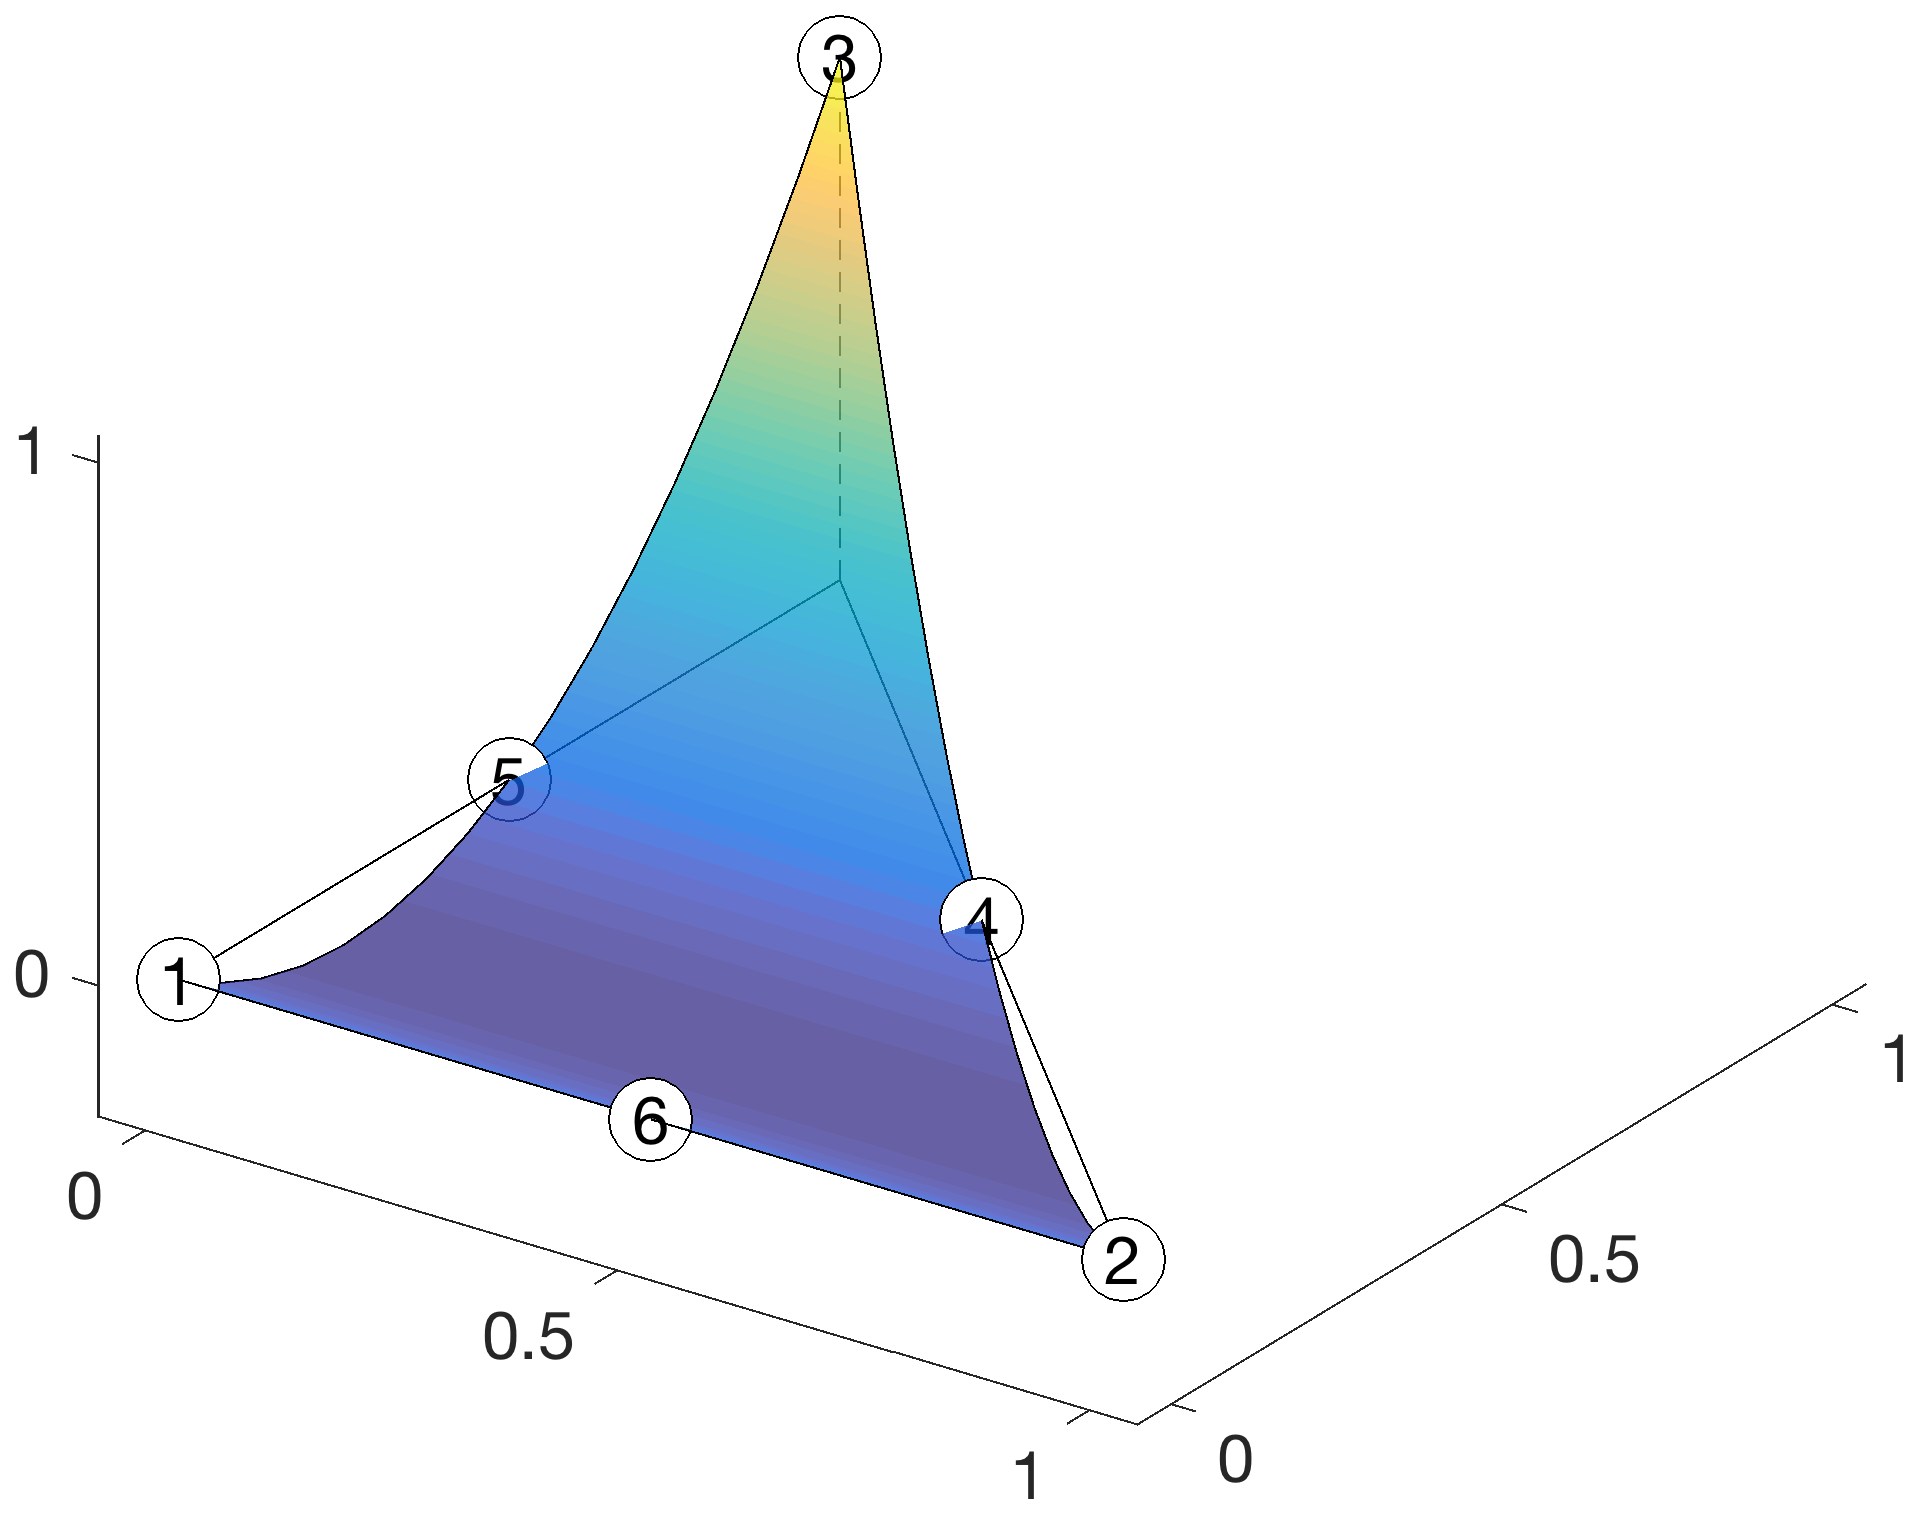
\includegraphics[width=0.3\textwidth]{shape_tri_p2_3}
  }
  \subfigure[$\tilde \phi_4$]{
    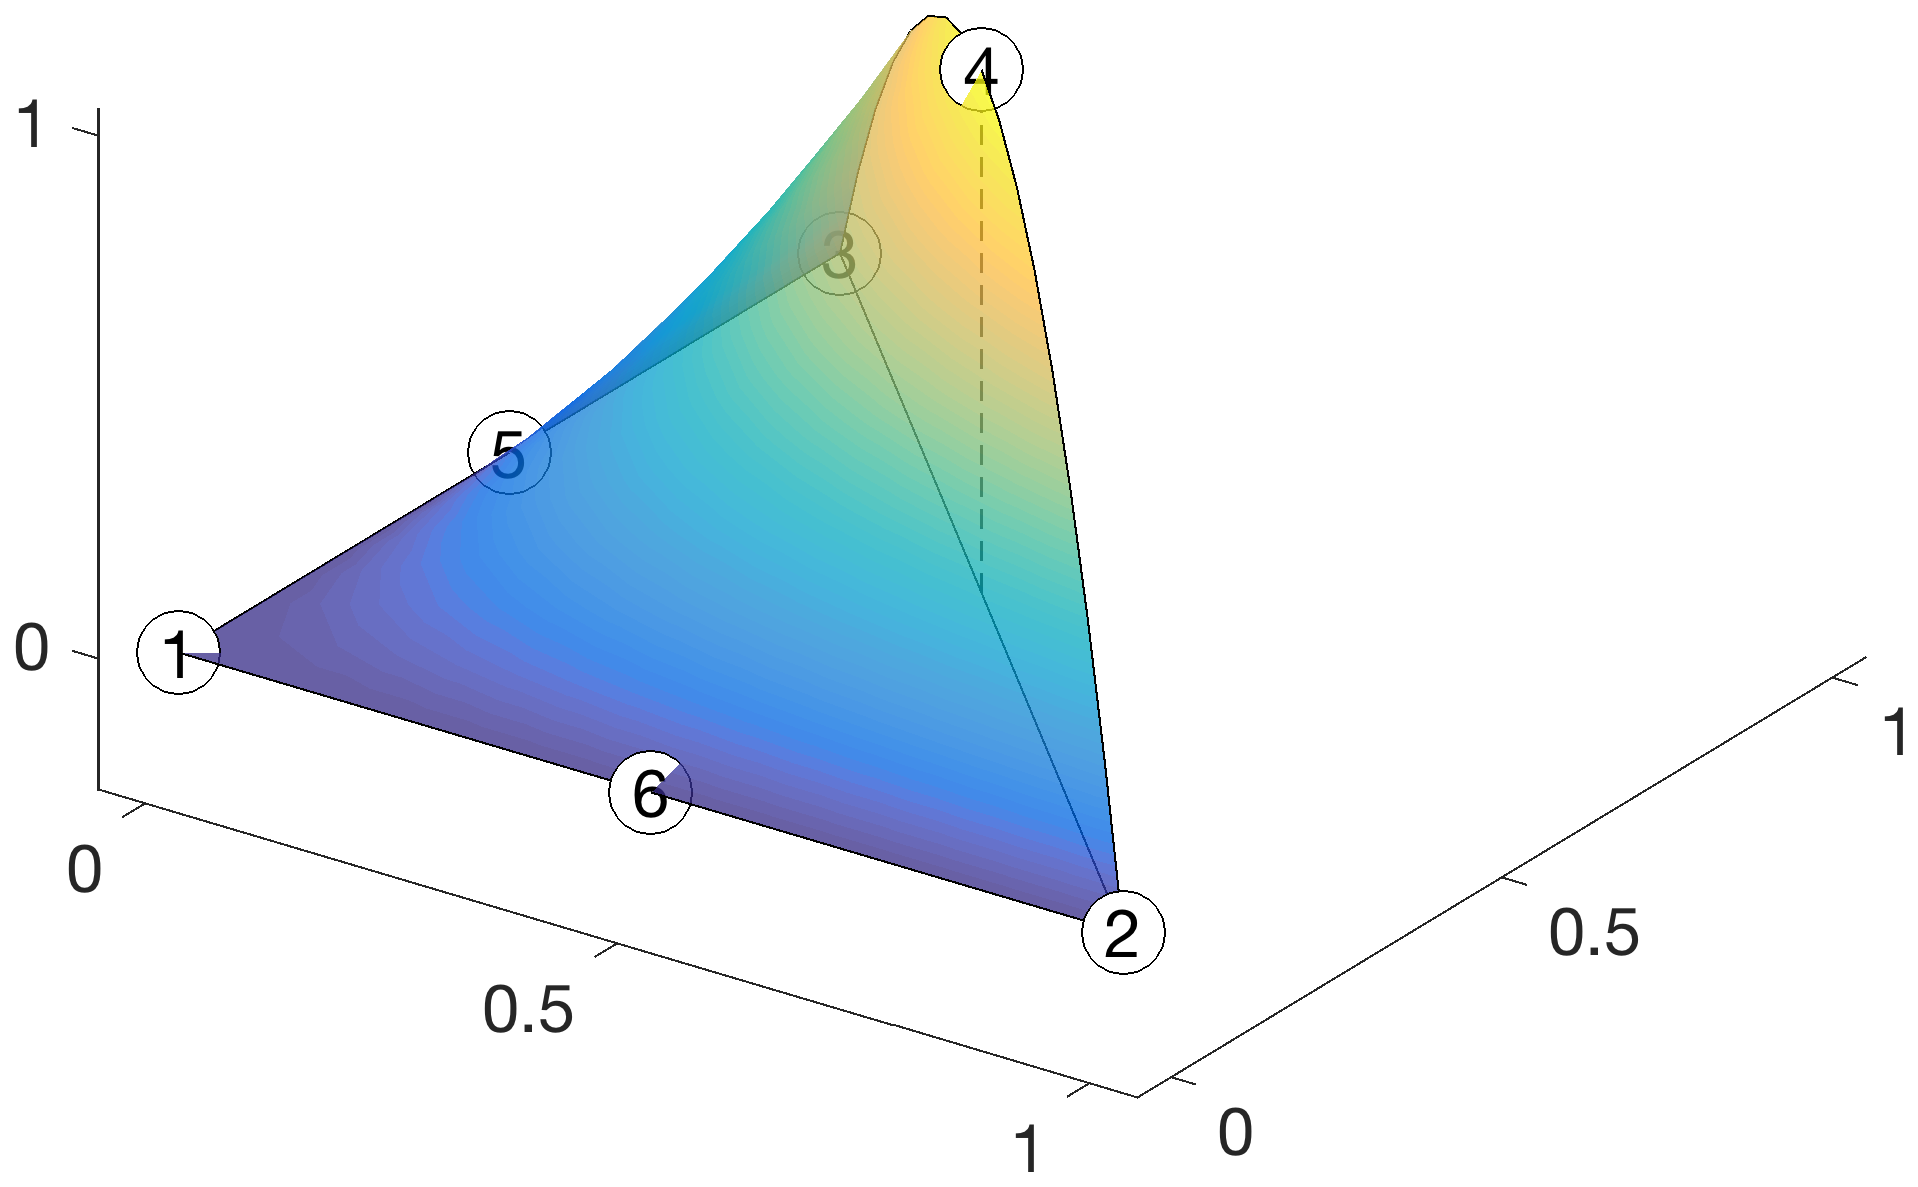
\includegraphics[width=0.3\textwidth]{shape_tri_p2_4}
  }
  \subfigure[$\tilde \phi_5$]{
    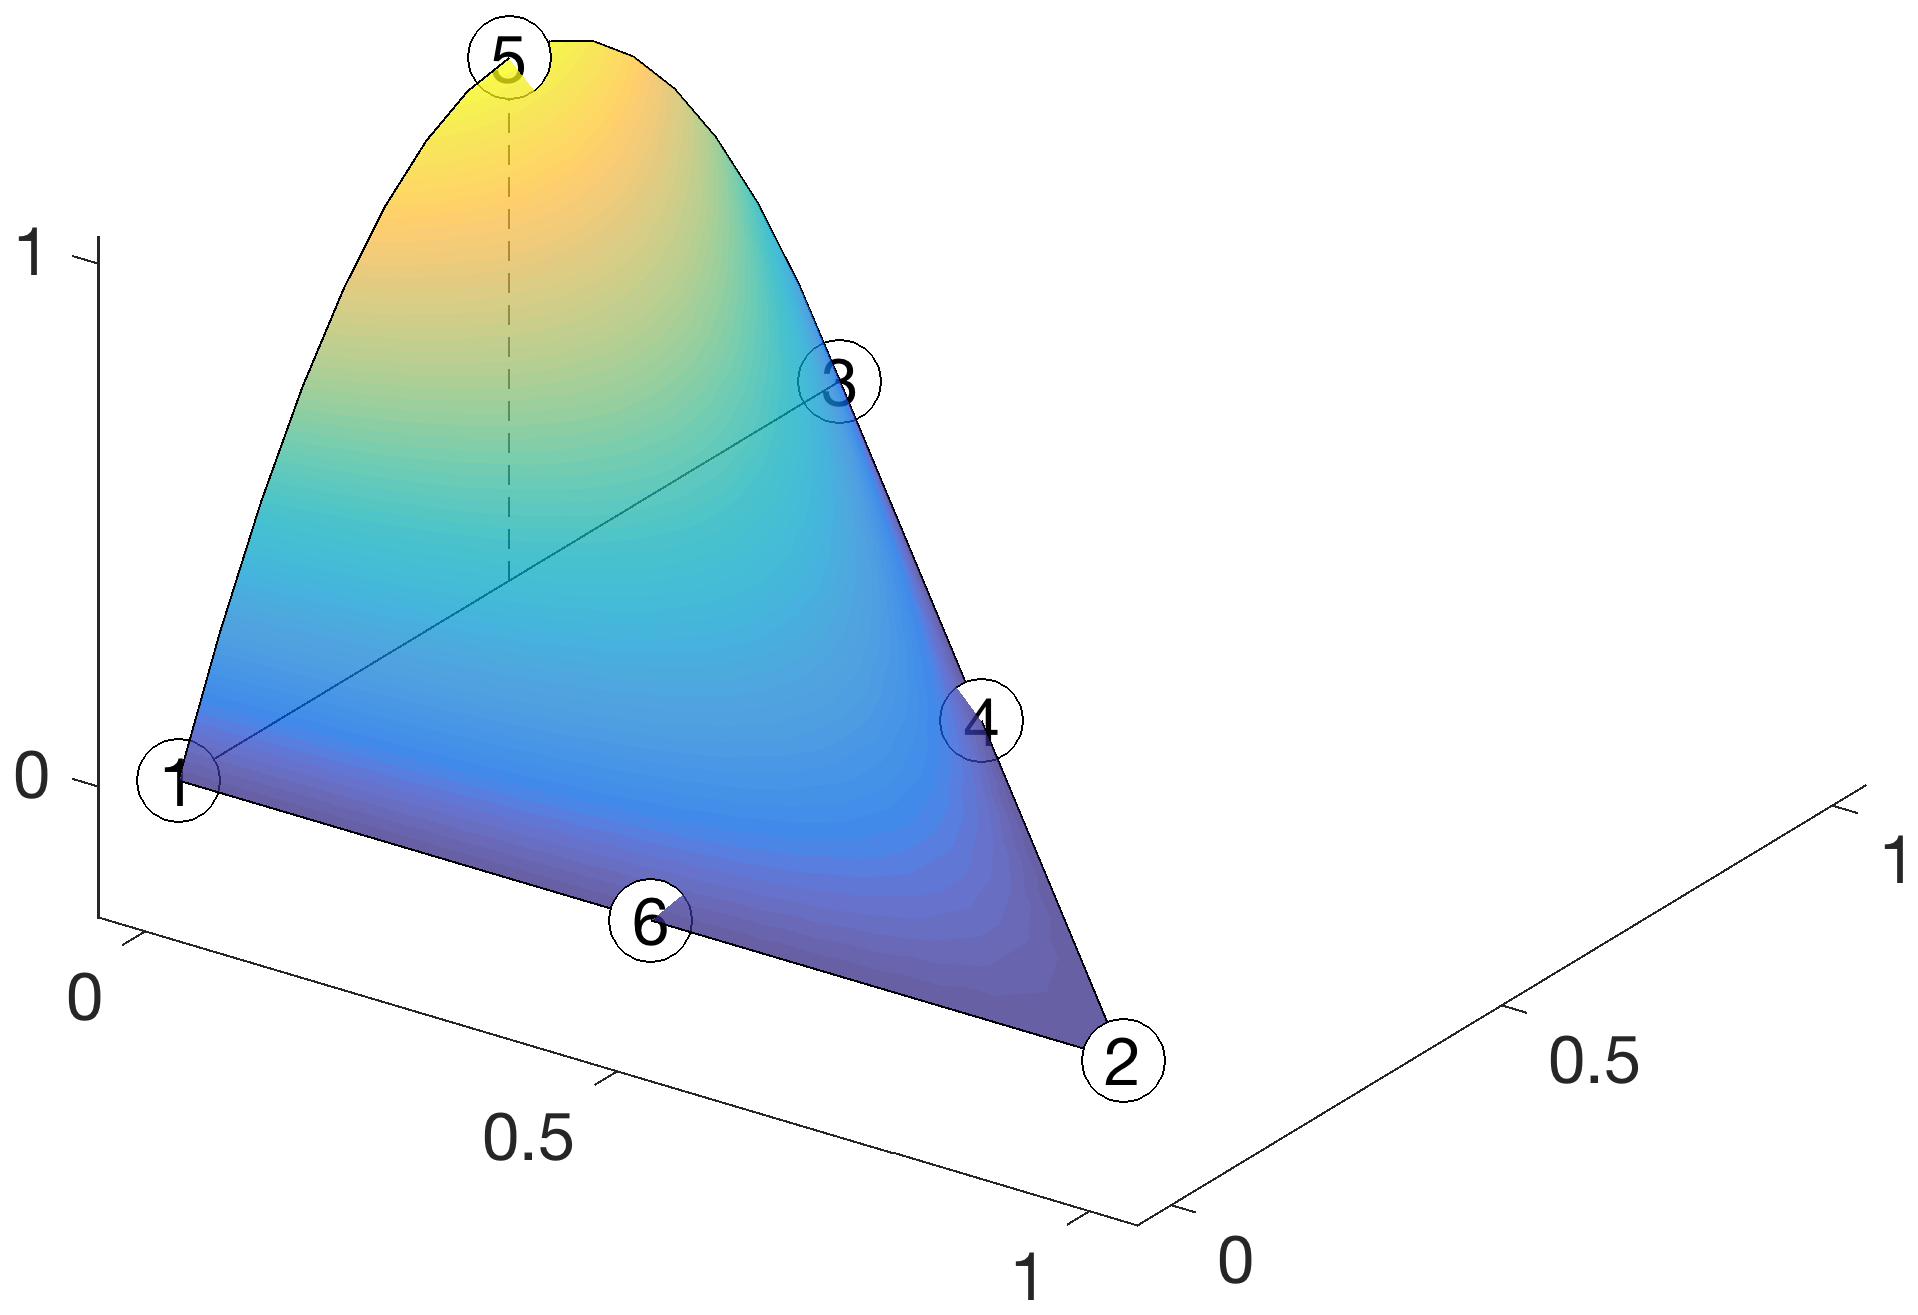
\includegraphics[width=0.3\textwidth]{shape_tri_p2_5}
  }
  \subfigure[$\tilde \phi_6$]{
    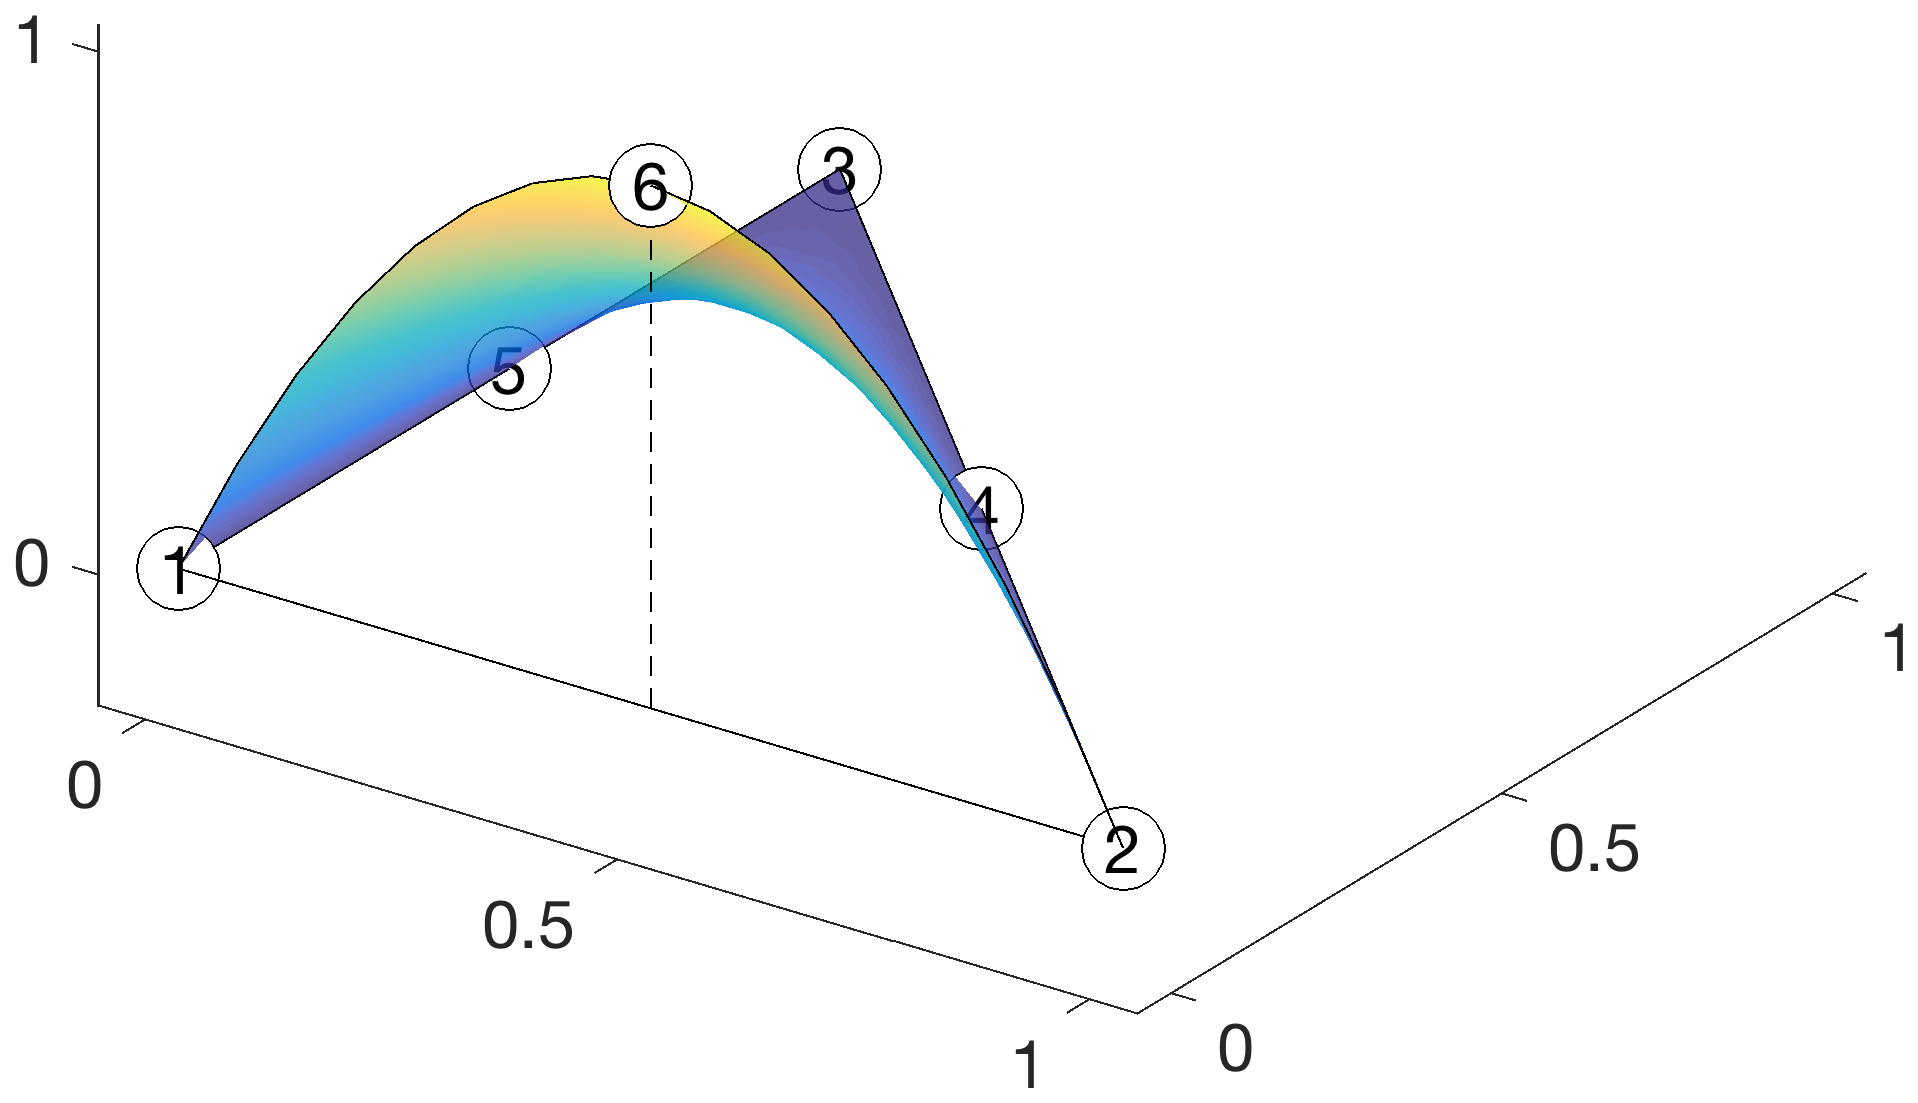
\includegraphics[width=0.3\textwidth]{shape_tri_p2_6}
  }
  \caption{Quadratic Lagrange shape functions on the reference triangle.}
  \label{fig:fe_shape_tri_p2}
\end{figure}
 The differentiation of~\eqref{eq:fe_quad_tri_rep} yields the gradient of the shape functions,
\begin{align*}
  \left. \pp{\tilde \phi_j}{\tilde x_1} \right|_{\tilde x} &= c^{(j)}_2 + 2 c^{(j)}_4 \tilde x^2_1 + c^{(j)}_5 \tilde x_2
  \\
  \left. \pp{\tilde \phi_j}{\tilde x_2} \right|_{\tilde x}&= c^{(j)}_3 + c^{(j)}_5 \tilde x_1 + 2 c^{(j)}_6 \tilde x_2.
\end{align*}
For the quadratic Lagrange element, the derivatives are linear functions, and they span $\PP^1(\tilde K)$.


As we have done for the linear Lagrange element in Section~\ref{sec:fe_lin_tri}, we now relates the node on a facet to nodes on the element. Figure~\ref{fig:fe_ref_tri_face_p2} shows the relationship between the nodes. Our facet-to-node map is 
\begin{equation*}
  \theta_{\tilde F\text{-}n} : \{ 1,2,3 \} \times \{ 1,2,3 \} \to \{ 1,\dots,6 \}
\end{equation*}
such that
\begin{align*}
  \theta_{\tilde F\text{-}n}(1,1) &= 2, & \theta_{\tilde F\text{-}n}(1,2) &= 3, & \theta_{\tilde F\text{-}n}(1,3) &= 4\\
  \theta_{\tilde F\text{-}n}(2,1) &= 3, & \theta_{\tilde F\text{-}n}(2,2) &= 1, & \theta_{\tilde F\text{-}n}(2,3) &= 5\\
  \theta_{\tilde F\text{-}n}(3,1) &= 1, & \theta_{\tilde F\text{-}n}(3,2) &= 2, & \theta_{\tilde F\text{-}n}(3,3) &= 6.
\end{align*}
As before, $j = \theta_{\tilde F\text{-}n}(i,k)$ is the Lagrange node on $\tilde T$ identified with the $k$-th Lagrange node of the facet $i$; i.e.,
\begin{equation*}
  \tilde z_{j \equiv\theta_{\tilde F\text{-}n}(i,k)}  = \tilde z^{\tilde F_i}_k \quad \forall i =1,2,3, \ k = 1,2,3.
\end{equation*}
We will make use of the mapping when the bilinear form or the linear form requires integration on a boundary.

\begin{figure}
  \centering
  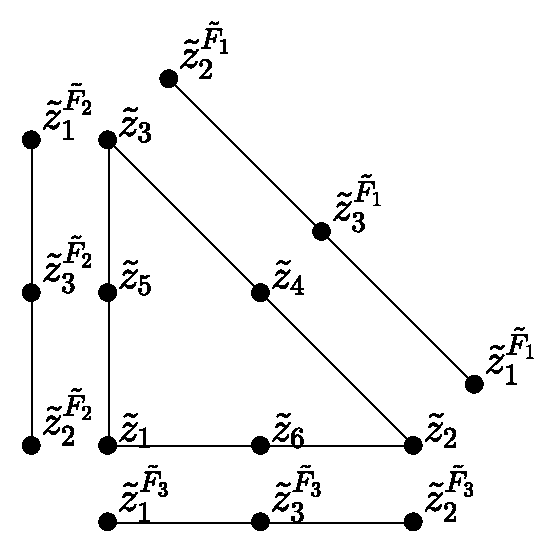
\includegraphics[width=0.35\textwidth]{ref_tri_face_p2}
  \caption{Quadratic Lagrange triangular element-facet relationship.}
  \label{fig:fe_ref_tri_face_p2}
\end{figure}

%% we now relate the trace of the shape functions on facets $F_i$, $i = 1,2,3$, to the shape functions on a line segment. We first note that any restriction of a two-dimensional quadratic function to a line segment is a quadratic function on the line segment.  We apply this principle to map the quadratic shape functions $\{\tilde \phi_j\}_{j=1}^6$ defined on a triangle $\tilde T \subset \RR^2$ to the quadratic shape functions $\{ \chi_k \}_{k=1}^3$ defined on a line segment $I \subset \RR^1$.

%% The mapping of the Lagrange nodes on the triangle $\tilde T$ to those on the facets $\{ \tilde F_i \}_{i=1}^3$ is shown in Figure~\ref{fig:fe_ref_tri_face_p2}. We note that the one-dimensional quadratic shape functions on the facet $\tilde F_1$, $\{ \chi_k^{\tilde F_1} \}_{k=1}^3$, are identified by the Lagrange nodes
%% \begin{equation*}
%%   \tilde z_1^{\tilde F_1} \equiv \tilde z_2 ,
%%   \quad
%%   \tilde z_2^{\tilde F_1} \equiv \tilde z_3 ,
%%   \quad \text{and} \quad
%%   \tilde z_3^{\tilde F_1} \equiv \tilde z_4 ,
%% \end{equation*}
%% and the shape functions are related by
%% \begin{equation*}
%%   \tilde \phi_2 |_{\tilde F_1} = \chi_1^{\tilde F_1} ,
%%   \quad
%%   \tilde \phi_3 |_{\tilde F_1} = \chi_2^{\tilde F_1} ,
%%   \quad \text{and} \quad
%%   \tilde \phi_4 |_{\tilde F_1} = \chi_3^{\tilde F_1} .
%% \end{equation*}
%% Analogous relationships exist for the facets $\tilde F_2$ and $\tilde F_3$. 
%% %% Similarly, on the facet $\tilde F_2$, the Lagrange nodes are
%% %% \begin{equation*}
%% %%   \tilde z_1^{\tilde F_2} \equiv \tilde z_3 \quad \text{and} \quad
%% %%   \tilde z_2^{\tilde F_2} \equiv \tilde z_1 ,
%% %% \end{equation*}
%% %% and the shape functions are related by
%% %% \begin{equation*}
%% %%   \tilde \phi_3 |_{\tilde F_2} = \chi_1^{\tilde F_2}
%% %%   \quad \text{and} \quad
%% %%   \tilde \phi_1 |_{\tilde F_2} = \chi_2^{\tilde F_2} ;
%% %% \end{equation*}
%% More compactly, we can introduce a facet-to-element node map
%% \begin{equation*}
%%   \theta_{\rm f-e} : \{1,2,3 \} \times \{1,2,3\} \to \{1,\dots,6\},
%% \end{equation*}
%% such that $j = \theta_{\rm f-e}(i,k)$ is the Lagrange node on $\tilde T$ identified with the $k$-th Lagrange node of the facet $i$. In other words,
%% \begin{equation*}
%%   \tilde z_k^{\tilde F_i} \equiv \tilde z_{\theta_{\rm f-e}(i,k)}, \quad k = 1,2, \ i = 1,2,3.
%% \end{equation*}
%% Accordingly, the trace of the two-dimensional shape functions $\{\tilde \phi_j\}_{j=1}^3$ are given related to the one-dimensional shape functions by
%% \begin{equation*}
%%   \tilde \phi_{\theta_{\rm f-e}(i,k)}|_{\tilde F_i} = \chi^{\tilde F_i}_k, \quad k = 1,2, \ i = 1,2,3.
%% \end{equation*}


\subsection{Generalization: an advanced method using Legendre polynomials}
\label{sec:fe_gen_shape}
We can generalize the procedure discussed so far in this section to generate Lagrange shape functions of an arbitrary degree on an arbitrary domain $\tilde K$.  Say we wish to generate Lagrange shape functions for a polynomial space of degree $p$ with a dimension $n_s$ and the interpolation nodes $\{ \tilde z_i \}_{i=1}^{n_s}$.  We first identify \emph{any} basis $\{ \tilde \psi_k \}_{k=1}^{n_s}$.  We then express the Lagrange shape functions as
\begin{equation}
  \tilde \phi_j(\tilde x) = \sum_{k=1}^{n_s} c^{(j)}_k \psi_k(\tilde x), \quad \tilde x \in \tilde K, \quad j = 1,\dots,n_s.
  \label{eq:fe_gen_val_rep}
\end{equation}
The coefficients that satisfy the interpolation condition $\tilde \phi_j(\tilde z_i) = \delta_{ij}$ must satisfy the $n_s \times n_s$ system
\begin{align}
  \bmat{ccc}
  \psi_1(\tilde z_1) & \cdots & \psi_{n_s}(\tilde z_1) \\
  \vdots & \ddots & \vdots \\
  \psi_1(\tilde z_{n_s}) & \cdots & \psi_{n_s}(\tilde z_{n_s}) 
  \emat
  \bmat{ccc}
  c^{(1)}_1 & \cdots & c^{(n_s)}_1 \\
  \vdots & \ddots & \vdots \\
  c^{(1)}_{n_s} & \cdots & c^{(n_s)}_{n_s}
  \emat
  =
  I_{n_s},
  \label{eq:fe_gen_coeff_sys}
\end{align}
where $I_{n_s}$ is the $n_s \times n_s$ identity matrix. The derivative of the shape functions are then given by
\begin{equation}
  \left. \pp{\tilde \phi_j}{\tilde x_i} \right|_{\tilde x}
  = \sum_{k=1}^{n_s} c^{(j)}_k \left. \pp{\tilde \psi_k}{\tilde x_i} \right|_{\tilde x}, \quad \tilde x \in \tilde K.
  \label{eq:fe_gen_der_rep}
\end{equation}
Note that this is a generalization, or simply an abstraction, of the method we have discussed for linear and quadratic shape functions on a line segment and triangle discussed in the previous sections.

The efficient implementation of this procedure relies on the efficient evaluation of the values and gradients of the basis functions $\{\tilde \psi_k \}_{k=1}^{n_s}$. One convenient choice for $\{\tilde \psi_k \}_{k=1}^{n_s}$ are the \emph{Legendre polynomials}, which is a set of orthogonal polynomials in $L^2(\tilde I)$. We provide a formal definition.
\begin{definition}[Legendre polynomial]
  \label{def:fe_legendre_poly}
  The Legendre polynomials $\{ \psi_i \}_{i=0}^{n}$ are hierarchical polynomials defined on a unit line segment $\tilde I \equiv (0,1)$ such that
  \begin{itemize}
  \item[(i)] $\text{span}\{ \psi_i \}_{i=0}^n = \PP^{n}(\tilde I)$  
  \item[(ii)] $(\psi_i,\psi_j)_{L^2(\Omega)} \equiv \int_{\tilde I} \psi_i \psi_j dx =  \delta_{ij}$, $\forall i,j = 1,\dots,n$. 
  \end{itemize}
\end{definition}
The orthogonality condition (ii) implies that the set $\{ \psi_i \}_{i=0}^{n}$ is linearly independent and hence is a basis for $\PP^n(\tilde I)$. In addition the Legendre polynomials of arbitrary degree and their respective derivatives can be evaluated using recurrence relations. We can hence use~\eqref{eq:fe_gen_val_rep} and \eqref{eq:fe_gen_der_rep} with the Legendre polynomials as the underlying basis.  In higher dimensions, we may use the tensor product of Legendre polynomials as the underlying basis.  The use of the Legendre polynomial as the underlying polynomials also ensures the linear system~\eqref{eq:fe_gen_coeff_sys} remains well-posed even if the polynomial degree is very high; the Vandermonde matrix associated with the monomials become ill-conditioned for a high-degree polynomials as the monomials becomes nearly linearly dependent.

%% \subsection{Computer implementation}
%% The procedure described in this section can be easily and efficiently implemented in any programming language. We here describe the procedure using a MATLAB-like language. The ingredients of the code are
%% \begin{itemize}
%% \item \texttt{interp\_nodes}.  The function returns an array of interpolation nodes $Z \in \RR^{n_s \times d}$ so that $Z_{ij} = \tilde z_{i,j}$ for a given reference domain and polynomial degree.
%% \item \texttt{monomial}. The input to the function is an array of evaluation points $X \in \RR^{n \times d}$ so that $X_{ij}$ is the $j$-th coordinate of the $i$-th evaluation. The function returns a matrix of function values $\Psi(X) \in \RR^{n \times n_s}$ so that $\Psi_{ij}(X) = \psi_j(x_i)$ and a order-3 tensor of derivative values $\nabla\Psi(X) \in \RR^{n \times n_s \times d}$ so that $(\nabla \Psi(X))_{ijk} = \left. \pp{\psi_j}{x_k} \right|_{x_i}$.  Here, $\psi_j$ is the $j$-th monomial basis function.  More generally $\{ \psi_j \}_{j=1}^{n_s}$ is underlying basis from which shape functions $\{ \phi_j \}_{j=1}^{n_s}$ are constructed; they could be, for example, (a tensor-product of) Legendre polynomials.
%% \end{itemize}
%% From these two functions, we can readily evaluate the values and gradients of Lagrange shape functions.  Our Vandermonde matrix $V \in \RR^{n_s \times n_s}$ associated with interpolation nodes $Z \in \RR^{n_s \times d}$ is given by
%% \begin{equation*}
%%   V = \Psi(Z) \quad (\text{in } \RR^{n_s \times n_s}).
%% \end{equation*}m
%% The Lagrange shape functions evaluated at the $n$ points associated with $X \in \RR^{n \times d}$ is given by $\Phi(X) \in \RR^{n \times n_s}$ such that
%% \begin{equation*}
%%   \Phi(X) = \Psi(X) V^{-1} \quad (\text{in } \RR^{n \times n_s}).
%% \end{equation*}
%% Here, $(\Phi(X))_{ij} = \phi_j(x_i)$, and we invoke the fact that the Vandermonde matrix $V$ is the inverse of the coefficient matrix $C$. Similarly, the derivative of the Lagrange shape functions 

  \section{Physical elements}
  \label{sec:fe_phy_elem}
\subsection{Geometry mapping}
\label{sec:fe_iso_map}
We have so far introduced shape functions $\{\tilde \phi_i\}_{i=1}^{n_s}$ defined on a reference element $\tilde K$, where the reference element may be the reference line segment $\tilde I$ or the reference triangle $\tilde T$. We now wish to construct shape functions $\{\phi_i\}_{i=1}^n$ which span the approximation space $\calV_h \subset \calV$.  To clearly distinguish between quantities defined on the reference domain and those defined on the actual physical domain, we will qualify the latter quantities with the adjective \emph{physical}. (Note that the quantities associated with the physical space, unlike those associated with the reference space, do not bear a tilde ($\tilde \cdot$).)

To begin, we create a mapping from a point $\tilde x$ in the reference element $\tilde K$ to a point $x$ in the physical element $K$.  The physical element is delineated by $n_s$ nodes, $\{ z^K_\alpha \}_{\alpha=1}^{n_s}$.  To map a point $\tilde x \in \tilde K$ in the reference domain to a point $x \in K$ in the physical domain, we employ a geometry mapping, $\calG^K: \tilde K \to K$ given by 
\begin{equation}
  x = \calG^K(\tilde x) \equiv \sum_{\alpha=1}^{n_s} z^K_\alpha \tilde \phi_\alpha(\tilde x) ,
  \label{eq:fe_iso_map}
\end{equation}
where $z^K_\alpha \in \RR^d$ is the coordinate of the $\alpha$-th node of the physical element $K$, $\tilde \phi_\alpha \in \PP^p(\tilde K)$ is the Lagrange shape function associated with the $\alpha$-th node of the reference element, and $n_s$ is the number of the shape functions.  Our geometry mapping $\calG^K: \tilde K \to K$ is a unique map that (i) is a polynomial map of degree $p$ and (ii) maps the Lagrange interpolation points $\{ \tilde z_\alpha \}_{\alpha}^{n_s}$ of the reference element $\tilde K$ to the respective Lagrange interpolation points $\{ z_\alpha \}_{\alpha}^{n_s}$ of the physical element $K$. The geometry mapping $\calG^K: \tilde K \to K$ is invertible under a reasonable condition; we will discuss the condition shortly.

An example of a $\PP^1$ geometry mapping of a triangle is shown in Figure~\ref{fig:fe_impl_isomap_p1}.  The physical domain $K_8$ is defined by the physical nodes $\{ z_1^{K_8}, z_2^{K_8}, z_3^{K_8} \}$ which are in turn identified by the three nodes of the mesh $\{ z_2, z_3, z_1 \}$.  Because the reference element is linear, the mapping $\calG^{K_8}: \tilde K \to K_8$ is affine.

\begin{figure}
  \centering
  \subfigure[triangulation]{
    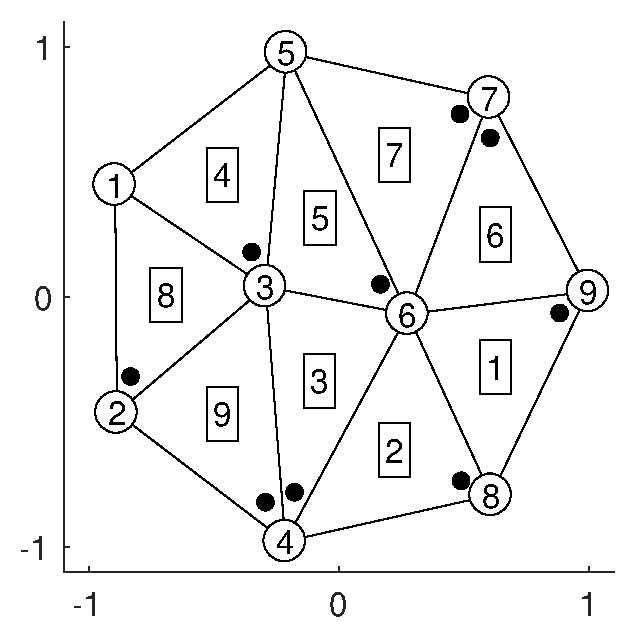
\includegraphics[width=0.3\textwidth]{fe_mesh_p1}
    \label{fig:fe_impl_mesh_p1}
  }
  \subfigure[reference domain $\tilde K \equiv \tilde T$]{
    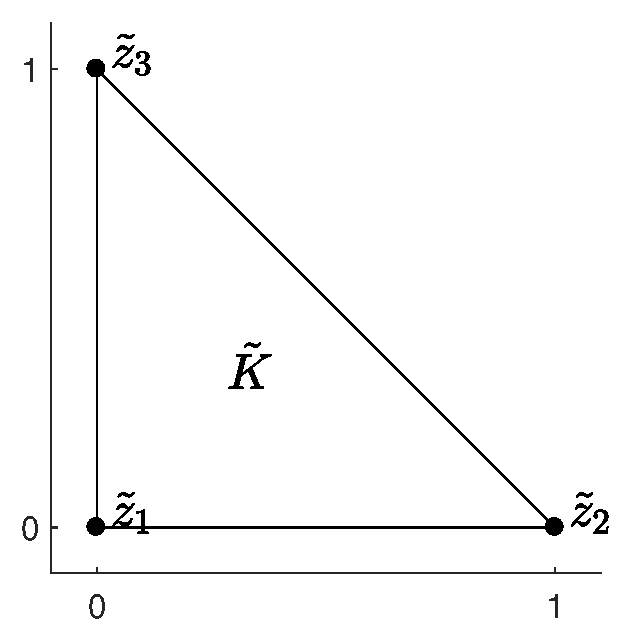
\includegraphics[width=0.3\textwidth]{isomap_p1_ref}
    %\label{fig:fe_impl_isomap_p1_ref}
  }
  \subfigure[physical domain $K_8$]{
    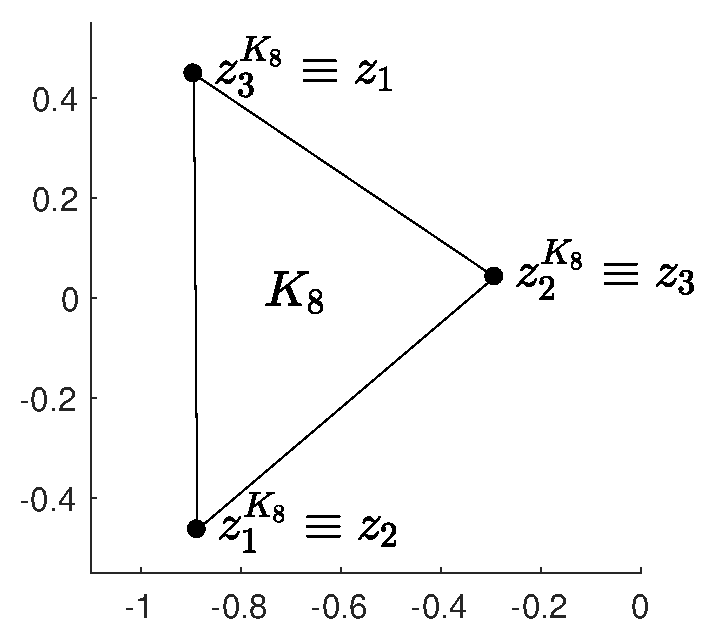
\includegraphics[width=0.33\textwidth]{isomap_p1_phy}
    %\label{fig:fe_impl_isomap_p1_phy}
  }
  \caption{$\PP^1$ geometry mapping. \label{fig:fe_impl_isomap_p1}}
\end{figure}

As an another example, we provide a $\PP^2$ geometry mapping of a triangle in Figure~\ref{fig:fe_impl_isomap_p2}. The physical domain $K_8$ is defined by the physical nodes $\{ z_1^{K_8}, z_2^{K_8}, z_3^{K_8}, z_4^{K_8}, z_5^{K_8}, z_6^{K_8} \}$ which are in turn identified by the six nodes of the mesh $\{ z_2, z_3, z_1, z_{11}, z_{10}, z_{13} \}$.  Because the reference element is quadratic, the mapping $\calG^{K_8}: \tilde K \to K_8$ is also quadratic.  We can represent curved geometries using $\PP^{p>1}$ geometry mapping; as we will see later, the accurate representation of the curved geometry is important to realize higher-order approximation of boundary value problems. 

\begin{figure}
  \centering
  \subfigure[triangulation]{
    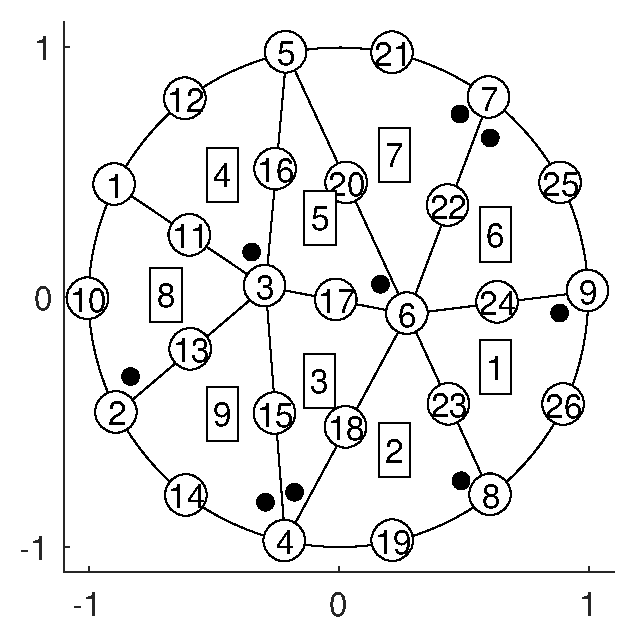
\includegraphics[width=0.3\textwidth]{fe_mesh_p2}
    \label{fig:fe_impl_mesh_p2}
  }
  \subfigure[reference domain $\tilde K \equiv \tilde T$]{
    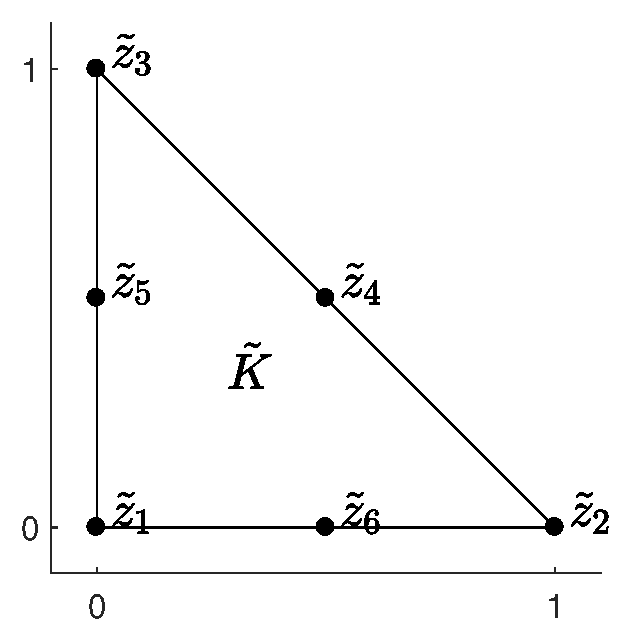
\includegraphics[width=0.3\textwidth]{isomap_p2_ref}
    %\label{fig:fe_impl_isomap_p1_ref}
  }
  \subfigure[physical domain $K_8$]{
    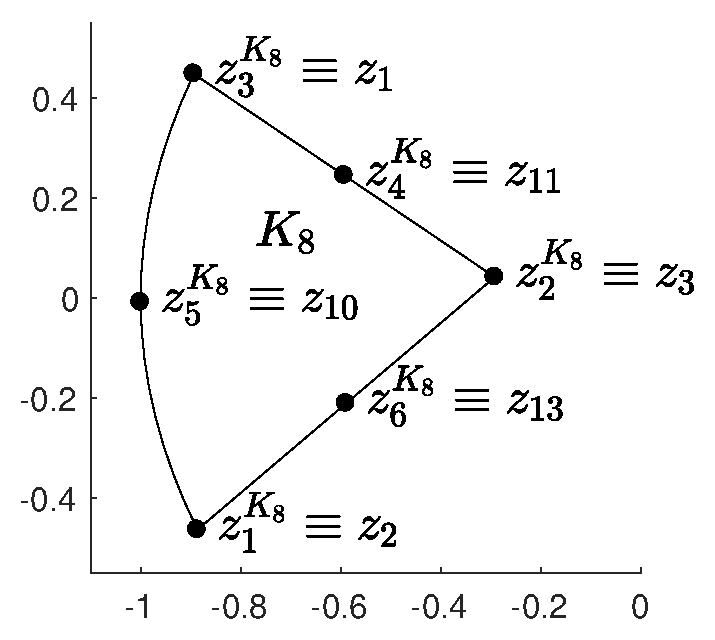
\includegraphics[width=0.33\textwidth]{isomap_p2_phy}
    %\label{fig:fe_impl_isomap_p1_phy}
  }
  \caption{$\PP^2$ geometry mapping. \label{fig:fe_impl_isomap_p2}}
\end{figure}

We now introduce a few quantities derived from the mapping.  We can differentiate the mapping~\eqref{eq:fe_iso_map} to evaluate the \emph{Jacobian} $J^K: \tilde K \to \RR^{d \times d}$ given by
\begin{equation*}
  J^K_{ij}(\tilde x)
  \equiv \left. \pp{x_i}{\tilde x_j} \right|_{\tilde x}
  = \left. \pp{\calG^K_i}{\tilde x_j} \right|_{\tilde x}
  = \sum_{\alpha= 1}^{n_s} z^K_{\alpha,i} \left. \pp{\tilde \phi_\alpha}{\tilde x_j} \right|_{\tilde x},
\end{equation*}
where $z^K_{\alpha,i}$ is the $i$-th coordinate of the $\alpha$-th node of element $K$. The Jacobian characterizes how an infinitesimal line segment $d\tilde l$ at $\tilde x \in \tilde K$ is mapped to an infinitesimal line segment $dl$ at $x \in K$; specifically, $dl = J^K d\tilde l$.  If the mapping $\calG^K: \tilde K \to K$ is a polynomial of degree $p$, the Jacobian $J^K: \tilde K \to \RR^{d \times d}$ is a polynomial of degree $p-1$. For a $\PP^1$ mapping, the Jacobian is constant over $\tilde K$.

The determinant of the Jacobian $\text{det}(J^K(\tilde x))$, or more compactly $|J^K(\tilde x)|$, relates the reference area $d \tilde x$ to the physical area $dx$ by
\begin{equation*}
  dx = |J^K(\tilde x)| d\tilde x.
\end{equation*}
If the mapping $\calG^K: \tilde K \to K$ is a polynomial of degree $p$, the Jacobian $J^K: \tilde K \to \RR^{d \times d}$ is a polynomial of degree $p-1$, and the determinant of the Jacobian $|J^K|: \tilde K \to \RR$ is a polynomial of degree $d(p-1)$.  For a $\PP^1$ mapping, the determinant of the Jacobian is constant over $\tilde K$.

Now we consider the \emph{inverse mapping} $(\calG^K)^{-1}: K \to \tilde K$, which maps a physical point $x \in K$ to a reference point $\tilde x \in \tilde K$.  The inverse mapping exists for all points if and only if
\begin{equation}
  |J^K(\tilde x)| > 0 \quad \forall \tilde x \in \tilde K.
  \label{eq:fe_iso_map_invcond}
\end{equation}
For a general polynomial mapping $\calG^K: \tilde K \to K$ of degree $p$, the condition must be checked for all $\tilde x \in \tilde K$. Moreover, the function $(\calG^K)^{-1}: K \to \tilde K$ is in general not a polynomial because the inverse of a polynomial is not a polynomial.  Consequently, he evaluation of the inverse mapping requires the solution of a nonlinear problem: given $x \in K$, find $\tilde x \in \tilde K$ such that $\calG^K(\tilde x) = x$.

The inverse mapping is greatly simplified for a $\PP^1$ mapping $\calG^K: \tilde K \to K$ because the Jacobian $J^K: \tilde K \to K$ is constant.  First, for a $\PP^1$ mapping, the condition \eqref{eq:fe_iso_map_invcond} is equivalent to the condition that (i) the area of the physical triangle is finite and (ii) the vertices are ordered in the counter-clock manner.  For a $\PP^1$ mapping, $|J^K|$ is constant and $|J^K|/2$ is the area of the physical triangle; the factor of $1/2$ is needed because the area of our reference triangle $\tilde T$ is $1/2$. Second, because $\calG^K: \tilde K \to K$ is linear, $(\calG^K)^{-1}: K \to \tilde K$ is also linear; given $x \in K$, we can find $\tilde x \in \tilde K$ by solving a linear problem. 

We can also compute the Jacobian associated with the inverse mapping, or the \emph{inverse Jacobian}, $(J^K)^{-1}: K \to \RR^{d \times d}$,
\begin{equation*}
  \left. \pp{\tilde x_i}{x_j} \right|_{\tilde x}
  = \left. \pp{(( \calG^K)^{-1})_i}{x_j} \right|_{\tilde x}
  = ((J^K(\tilde x))^{-1})_{ij}.
\end{equation*}
The algebraic inverse of the Jacobian $J^K = \pp{x}{\tilde x}$ is the inverse Jacobian $(J^K)^{-1} = \pp{\tilde x}{x}$. The inverse Jacobian $\pp{x_i}{\tilde x_j}$ is well defined at $\tilde x \in \tilde K$ if and only if $|J^K(\tilde x)| > 0$. For a general polynomial mapping $\calG^K: \tilde K \to K$ of degree $p$, the inverse Jacobian is not a polynomial because the inverse of a polynomial is in general not a polynomial.  For a $\PP^1$ mapping, the inverse Jacobian $(J^K)^{-1}: K \to \RR^{d \times d}$ is constant because the Jacobian $J^K: \tilde K \to \RR^{d \times d}$ is constant.

\subsection{Physical shape functions}
  \label{sec:fe_phy_shape}
Given an geometry mapping $\calG^K : \tilde K \to K$, we now introduce physical shape functions $\{ \phi^K_\alpha \}_{\alpha=1}^{n_s}$ associated with the physical element $K \in \calT_h$.  We choose the basis functions that satisfy
\begin{equation}
  \phi^K_\alpha(x = \calG^K(\tilde x)) = \tilde \phi_\alpha(\tilde x) \quad \forall \tilde x \in \tilde K, \quad \alpha =  1, \dots, n_s,
  \label{eq:fe_impl_phiK}
\end{equation}
where $\tilde x \mapsto x = \calG^K(\tilde x)$ is provided by the geometry mapping~\eqref{eq:fe_iso_map}. In words, the physical basis function $\phi^K_\alpha$ evaluated at the physical point $x(\tilde x) \in K$ takes on the same value as the associated reference basis function $\phi_\alpha$ evaluated at the associated reference point $\tilde x \in \tilde K$.

We can also differentiate~\eqref{eq:fe_impl_phiK} to obtain the derivative of the physical basis functions in the physical space: given any $\tilde x \in \tilde K$, 
\begin{equation}
  \left. \pp{\phi^K_\alpha}{x_i} \right|_{x = \calG^K(\tilde x)} =
  \sum_{j=1}^{d} \pp{\tilde x_j}{x_i} \left. \pp{\tilde \phi_\alpha}{\tilde x_j} \right|_{\tilde x}  \quad i = 1,\dots,d, \ \alpha = 1,\dots,n_s.
  \label{eq:fe_impl_dphiK}
\end{equation}
The relationship may be expressed more explicitly using matrices and vectors; for $d = 2$,
\begin{equation*}
  \bmat{c}
  \pp{\phi_\alpha^K}{x_1} \\ \pp{\phi_\alpha^K}{x_2}
  \emat_{x = \calG^K(\tilde x)}
  =
  \bmat{cc}
  \pp{\tilde x_1}{x_1} & \pp{\tilde x_2}{x_1} \\
  \pp{\tilde x_1}{x_2} & \pp{\tilde x_2}{x_2}
  \emat_{\tilde x}
  \bmat{c}
  \pp{\tilde \phi_\alpha}{\tilde x_1} \\ \pp{\tilde \phi_\alpha}{\tilde x_2}
  \emat_{\tilde x}.
\end{equation*}
Or, noting that $\pp{\tilde x_j}{x_i} = ((J^K)^{-1})_{ji} = ((J^K)^{-T})_{ij}$, a more compact expression (for any $d$) is
\begin{equation}
  \nabla \phi_\alpha^K(x = \calG^K(\tilde x)) = (J^K)^{-T}(\tilde x) \tilde \nabla \tilde \phi_\alpha(\tilde x).
  \label{eq:fe_impl_dphiK_2}
\end{equation}
Expressions~\eqref{eq:fe_impl_phiK} and \eqref{eq:fe_impl_dphiK} (or equivalently \eqref{eq:fe_impl_dphiK_2}) allows us to evaluate the value and gradient, respectively, of the physical shape function $\phi^K_\alpha$ at a physical point $x = \calG^K(\tilde x) \in K$ associated with a select reference point $\tilde x \in \tilde K$; we will soon see this is exactly the capability we need to evaluate stiffness matrices and load vectors.

As an example, consider the physical element $K_9$ in the triangulation shown in Figure~\ref{fig:fe_impl_mesh_p1} comprises linear elements.  The element $K_9$ is delineated by the nodes $\{ z^{K_9}_1 = z_4, z^{K_9}_2 = z_3, z^{K_9}_3 = z_2 \}$. The reference shape function $\tilde \phi_2 \in \PP^1(\tilde T)$ maps to the physical shape function $\phi_2^{K_9}$ as shown in Figure~\ref{fig:fe_impl_shape_map_p1}.  We in fact recognize that $\phi_2^{K_9}$ is the restriction of the physical (global) shape function $\phi_3$ associated with $z_3$; formally, $\phi_2^{K_9} \equiv \phi_3|_{K_9}$. %Because the shape function is linear and the geometry mapping is linear, the physical shape function is a linear function: $\phi_i^{K_9} \in \PP^1(K_9)$, $i = 1,\dots,3$.


%% As an example, consider the triangulation shown in Figure~\ref{fig:fe_impl_mesh_p1}.  The physical element $K_5 \in \calT_h$ is delineated by the nodes
%% \begin{equation*}
%%   z^{K_5}_1 = v_6 = (0.28,-0.07), \quad 
%%   z^{K_5}_2 = v_5 = (-0.21,0.98), \quad \text{and} \quad
%%   z^{K_5}_3 = v_3 = (-0.29,0.04);
%% \end{equation*}
%% we recall that the dot ($\bullet$) in Figure~\ref{fig:fe_mesh_p1} denotes the first vertex of the physical element, and vertices are in the counter-clockwise order. The third reference basis function $\tilde \phi_3$ over $\tilde K$ is shown in Figure~\ref{fig:fe_impl_loc_shape}.  The associated physical basis function $\phi_3^{K_5}$ over $K_5 \in \calT_h$ is shown in Figure~\ref{fig:fe_impl_glob_shape}.  Note that the $\phi_3^{K_5}$ is by definition defined over only $K_5 \subset \Omega$ and not the entire $\Omega$.

\begin{figure}
  \centering
  \subfigure[reference shape function $\tilde \phi_2$]{
    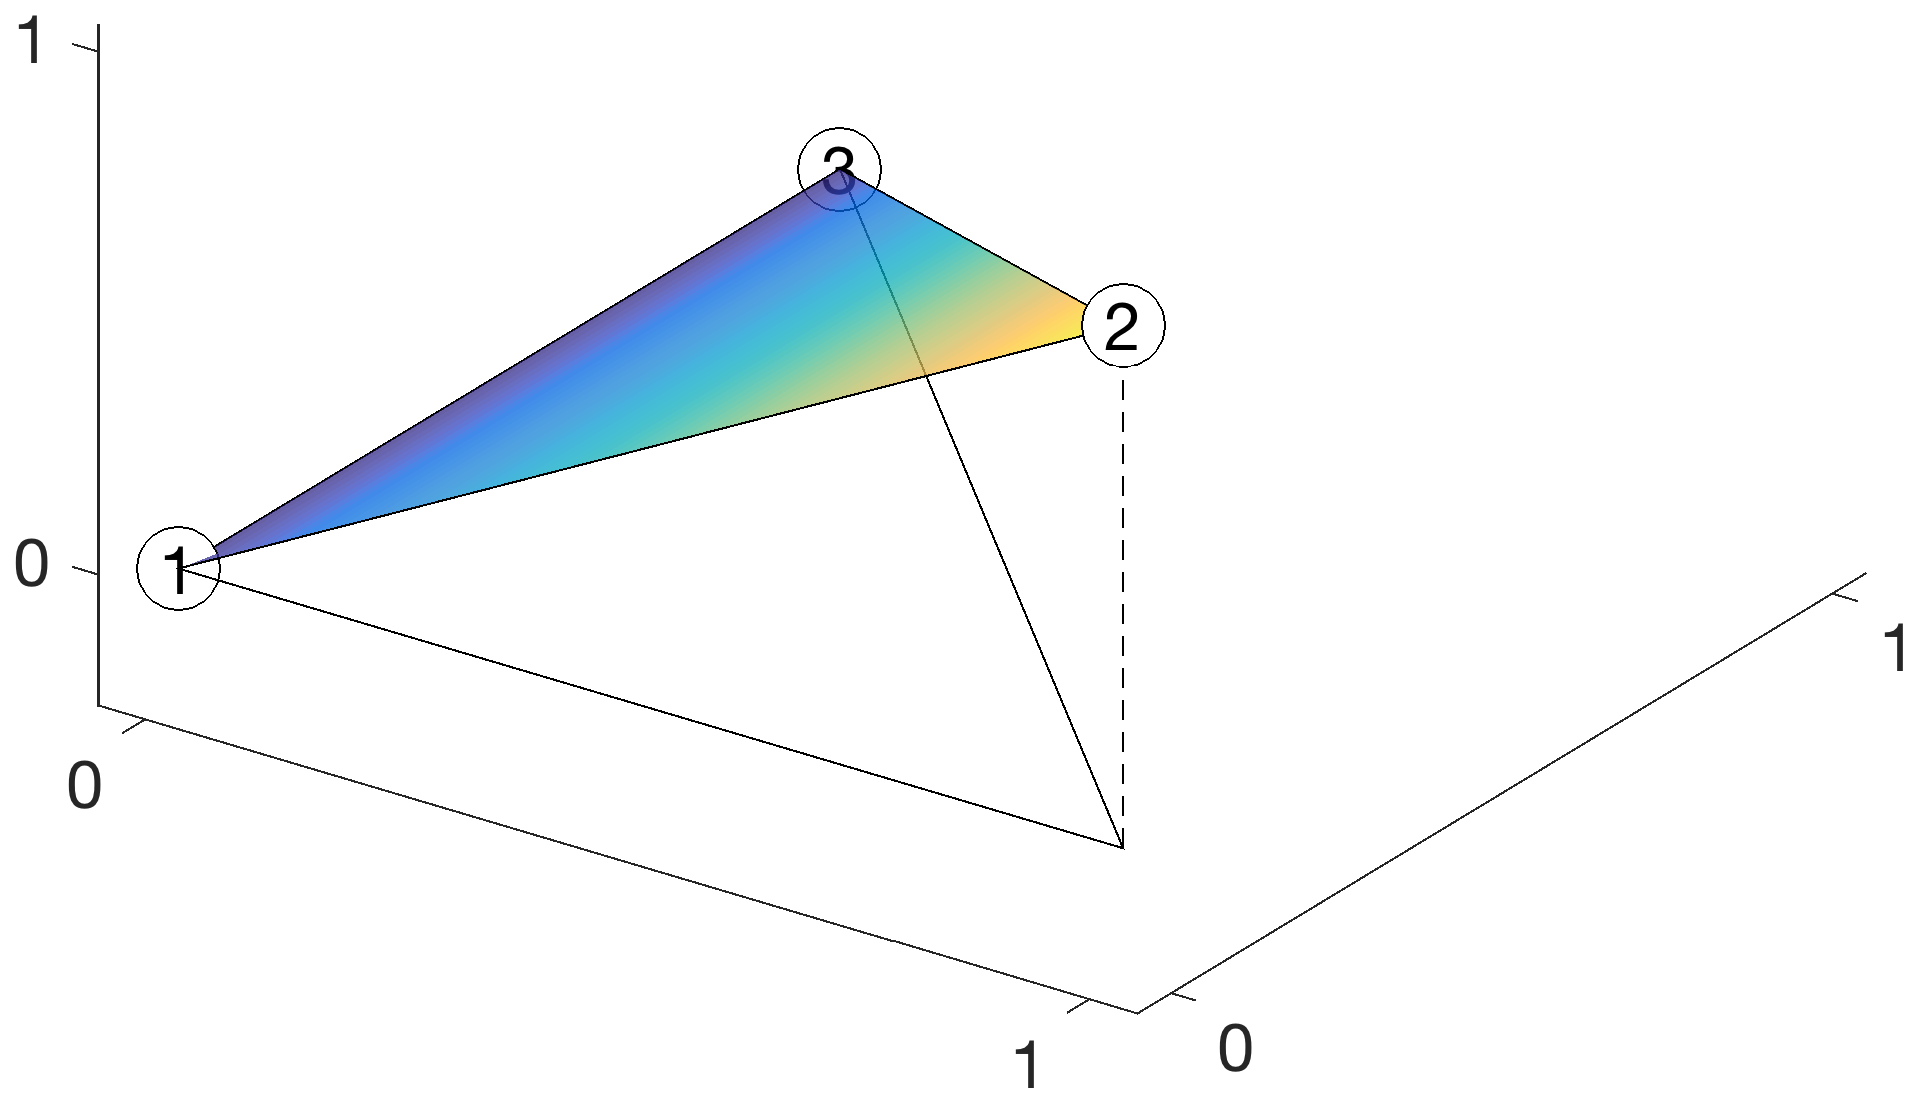
\includegraphics[width=0.3\textwidth]{shape_tri_p1_2}
    \label{fig:fe_impl_loc_shape_p1}
  }
  \subfigure[physical shape function $\phi^{K_9}_2$]{
    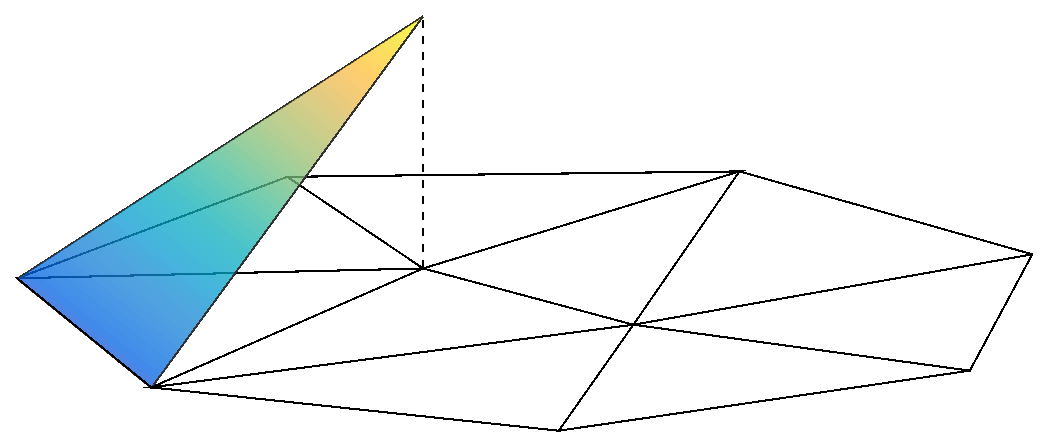
\includegraphics[width=0.33\textwidth]{shape_global_p1_part}
    \label{fig:fe_impl_glob_shape_p1}
  }
  \caption{Mapping of shape functions for a $\PP^1$ element.}
  \label{fig:fe_impl_shape_map_p1}
\end{figure}


As another example, consider the physical element $K_9$ in the triangulation shown in Figure~\ref{fig:fe_impl_mesh_p2} comprises quadratic elements. The element $K_9$ is delineated by the nodes $\{ z^{K_9}_1 = z_4, z^{K_9}_2 = z_3, z^{K_9}_3 = z_2,  z^{K_9}_4 = z_{13},  z^{K_9}_5 = z_{14},  z^{K_9}_6 = z_{15} \}$.  The reference shape function $\tilde \phi_2 \in \PP^2(\tilde T)$ maps to the physical shape function $\phi_2^{K_9}$ as shown in Figure~\ref{fig:fe_impl_shape_map_p2}.  We again recognize that $\phi_2^{K_9}$ is the restriction of the physical (global) shape function $\phi_3$ associated with $z_3$; formally, $\phi_2^{K_9} \equiv \phi_3|_{K_9}$.

\begin{figure}
  \centering
  \subfigure[reference shape function $\tilde \phi_2$]{
    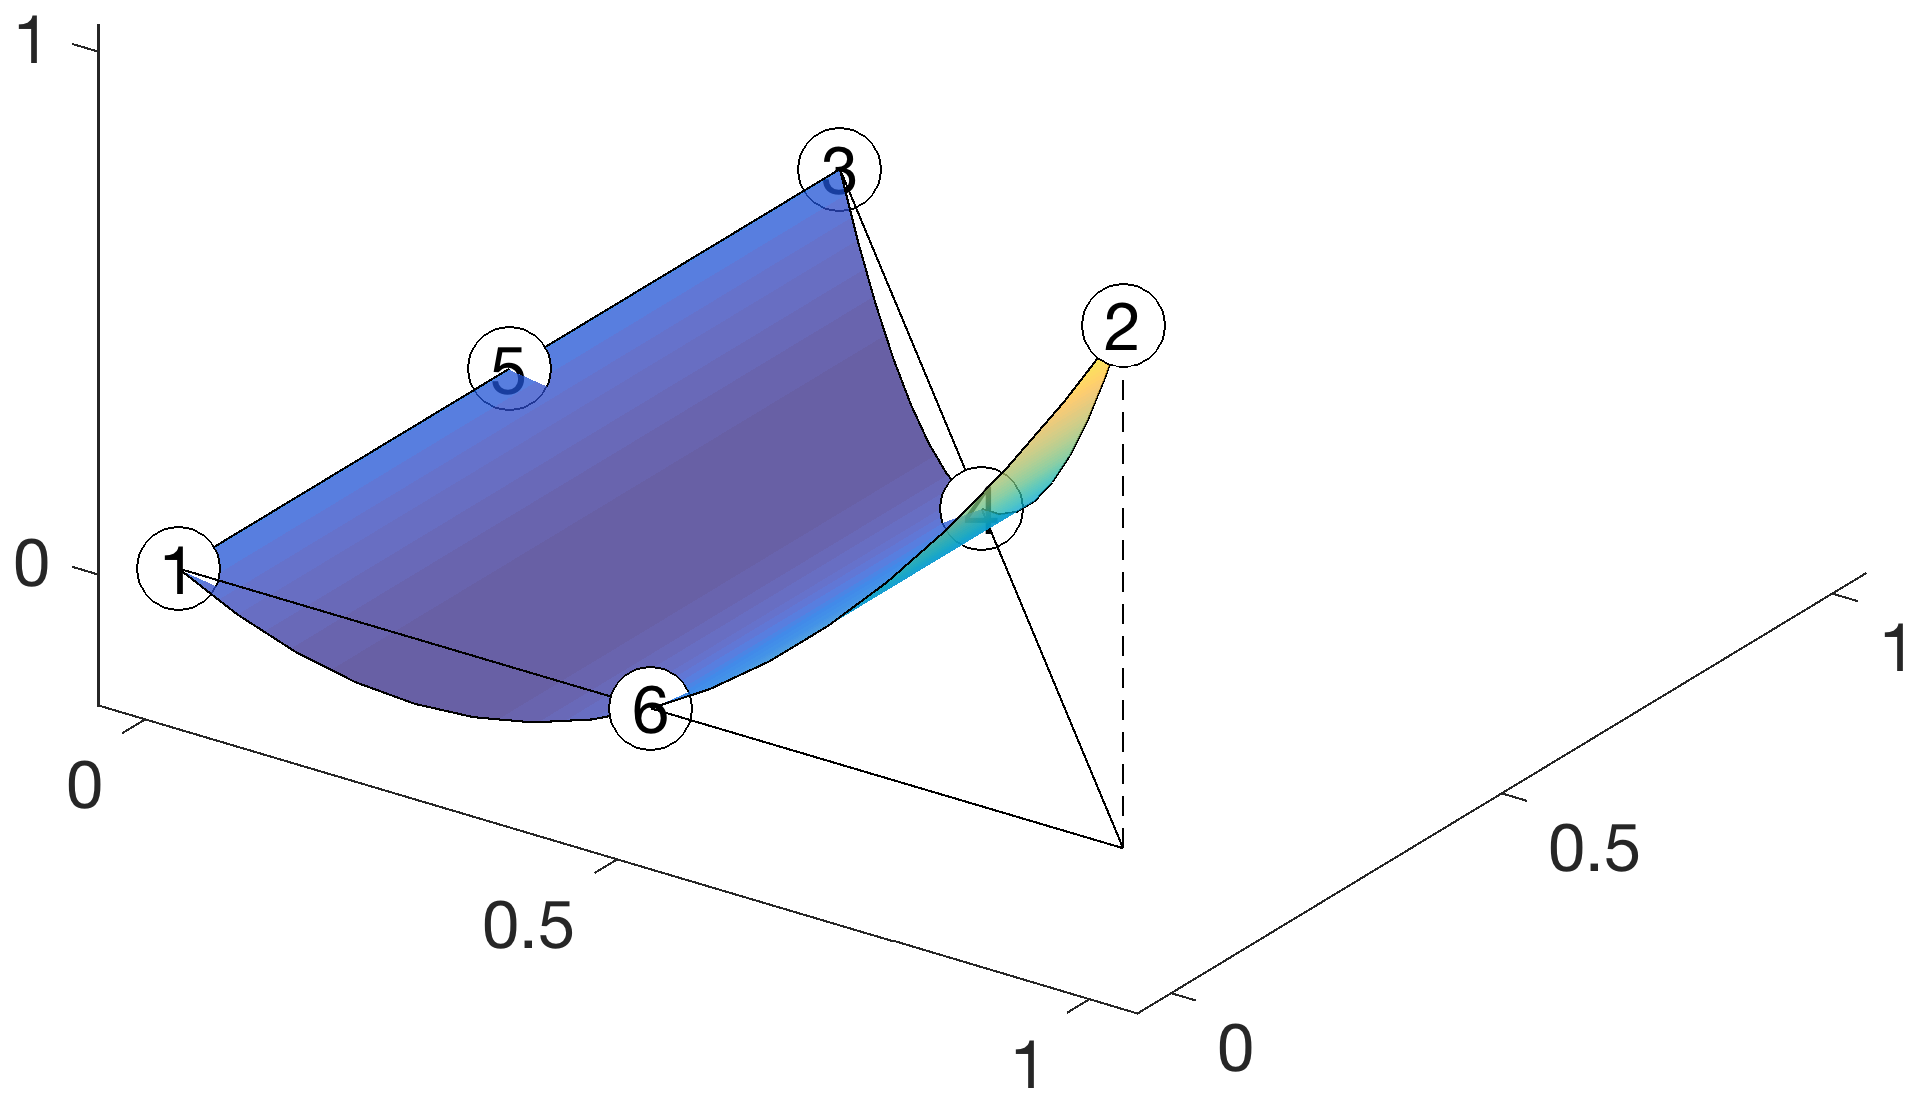
\includegraphics[width=0.3\textwidth]{shape_tri_p2_2}
    \label{fig:fe_impl_loc_shape_p2}
  }
  \subfigure[physical shape function $\phi^{K_9}_2$]{
    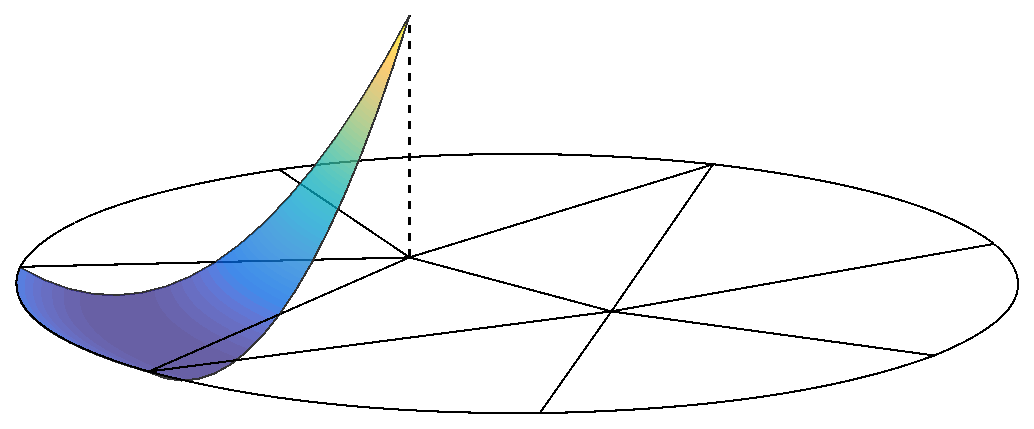
\includegraphics[width=0.33\textwidth]{shape_global_p2_part}
    \label{fig:fe_impl_glob_shape_p2}
  }
  \caption{Mapping of shape functions for a $\PP^2$ element.}
  \label{fig:fe_impl_shape_map_p2}
\end{figure}

We make one remark about our physical basis functions defined by~\eqref{eq:fe_impl_phiK}.  Even though the reference basis function $\tilde \phi: \tilde K \to \RR$ is a polynomial in $\tilde K$, the physical basis function $\phi^K_\alpha: K \to \RR$ is in general not a polynomial in $K$. To see this, we observe that $\phi^K_\alpha(x) = \tilde \phi_\alpha((\calG^K)^{-1}(x))$, $\forall x \in K$; because the inverse map $(\calG^K)^{-1}: K \to \tilde K$ is not a polynomial in $K$ for a $\PP^{p>1}$ geometry mapping, the function $\phi^K_\alpha(\cdot) = \tilde \phi_\alpha((\calG^K)^{-1}(\cdot)) = \tilde \phi_\alpha \circ (\calG^K)^{-1}$ is not a polynomial in $K$.  Conversely, we note that $\phi^K_\alpha(\calG(\cdot)) = \phi^K_\alpha \circ \calG^K = \tilde \phi(\cdot)$ \emph{is} a polynomial in $\tilde K$. Hence, in the presence of curved elements, approximation space is not
\begin{equation*}
  \calV_h \equiv \{ v \in H^1(\Omega) \ | v|_K \in \PP^p(K), \ \forall K \in \calT_h \}
\end{equation*}
but rather
\begin{equation*}
  \calV_h \equiv \{ v \in H^1(\Omega) \ | \ v|_K \circ \calG^K \in \PP^p(\tilde K), \ \forall K \in \calT_h \}.
\end{equation*}
However, for a $\PP^1$ geometry mapping, the notation is simplified; because the inverse mapping $(\calG^K)^{-1}: K \to \tilde K$ is affine, the physical shape function $\phi^K_\alpha(\cdot) = \tilde \phi_\alpha((\calG^K)^{-1}(\cdot))$ is a polynomial in $K$.

%Using these basis functions, we can represent any function 
%given $\tilde x \in \tilde K$,
%\begin{equation*}
%  v(x(\tilde x))
  %= \tilde v(\tilde x)
%  = \sum_{\alpha = 1}^{n_s} \hat v_\alpha \phi^K_\alpha(x(\tilde x))
%\end{equation*}
%\begin{equation*}
%  \left. \pp{v}{x} \right|_{x(\tilde x)} 
  % = \left. \pp{\tilde v}{\tilde x} \right|_{\tilde x} \left. \pp{\tilde x}{x} \right|_{\tilde x}
%  = \sum_{\alpha = 1}^{n_s} \hat v_\alpha \left. \pp{\phi^K_\alpha}{x} \right|_{x(\tilde x)}
%\end{equation*}


Before we conclude this section, we clarify the nomenclature.  In this section, we considered physical elements that results from using the same polynomial space for the geometry mapping $\calG: \tilde K \to K$ and the function representation; these elements are called \emph{isoparametric elements}. In general, the polynomials used for the geometry mapping and function representation need not be the same.   An element that uses a higher degree representation of the geometry than functions is called a \emph{superparametric element}. Conversely, an element that use a lower degree representation of the geometry than functions is called a \emph{subparametric element}.

\subsection{Geometry mapping for the facets}
In Section~\ref{sec:fe_iso_map}, we introduced an geometry mapping $\calG^K: \tilde K \to K$ from a reference element $\tilde K \subset \RR^d$ to a physical element $K \subset \RR^d$.  While this is the only mapping we need to evaluate bilinear and linear forms that only require integration over $\Omega$, forms that require integration over boundaries --- for example a Neumann boundary $\Gamma_N \subset \partial \Omega$ --- requires another mapping. Specifically, we require a mapping from a $(d-1)$-dimensional reference element to the associated physical facet that lies in a $d$-dimensional space; the physical facet is a $d-1$-dimensional manifold embedded in a $d$-dimensional space.  For concreteness, in this section we restrict ourselves to the case $d=2$, and consider the geometry mapping $\calG^F: \tilde I \to F$ from the reference line segment $\tilde I \subset \RR^1$ to a physical facet $F \subset \RR^2$ of a triangle.

Figure~\ref{fig:fe_impl_isomap_face_p2} shows a concrete example of an geometry mapping from a reference line segment $\tilde I$ to a physical facet $F$, the second facet of the physical element $K_8$.  We recall from Section~\ref{sec:fe_p2_tri} that the Lagrange nodes on the reference facet $\tilde F_{i \equiv2}$ are related to those on the reference element $\tilde T$ by $\tilde z_\alpha = \tilde z^{\tilde F_{i\equiv 2}}_\gamma$ for $\alpha = \theta_{\tilde F\text{-}n}(i \equiv 2,\gamma)$, $\gamma = 1,2,3$; for the case in Figure~\ref{fig:fe_impl_isomap_face_p2}, we obtain $\{ \tilde z_1^{\tilde F_2} \equiv \tilde z_3, \tilde z_2^{\tilde F_2} \equiv \tilde z_1, \tilde z_3^{\tilde F_2} \equiv \tilde z_5 \}$.  Accordingly, the Lagrange nodes on the physical facet $F$ are related to those on the physical element $\{z^{K_8}_j\}_{j=1}^6$, and the (global) nodes $\{z_i\}_{i=1}^n$,  by $\{z_1^{F)} \equiv z^{K_8}_3 \equiv z_1, z_2^{F} \equiv z^{K_8}_1 \equiv z_2, z_3^{F} \equiv z^{K_8}_5 \equiv z_{10} \}$. 
\begin{figure}
  \centering
  \subfigure[triangulation]{
    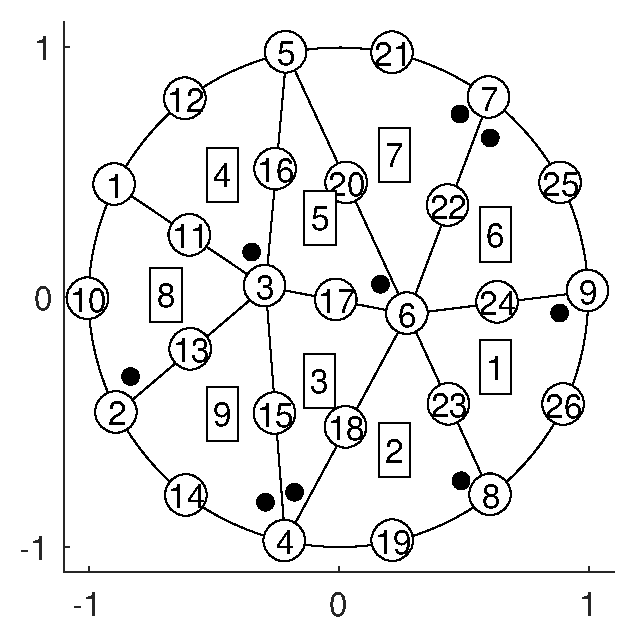
\includegraphics[width=0.3\textwidth]{fe_mesh_p2}
  }
  \subfigure[reference line segment $\tilde K \equiv \tilde I$]{
    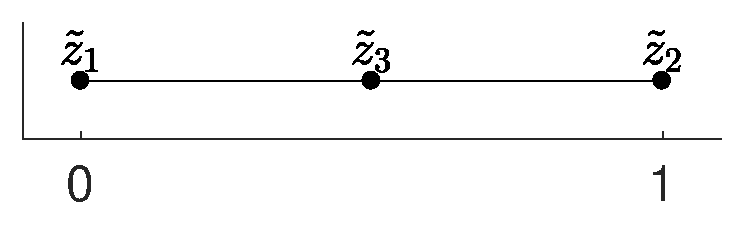
\includegraphics[width=0.3\textwidth]{isomap_p2_ref_edge}
    %\label{fig:fe_impl_isomap_p1_ref}
  }
  \subfigure[physical facet $F(K_8,2)$]{
    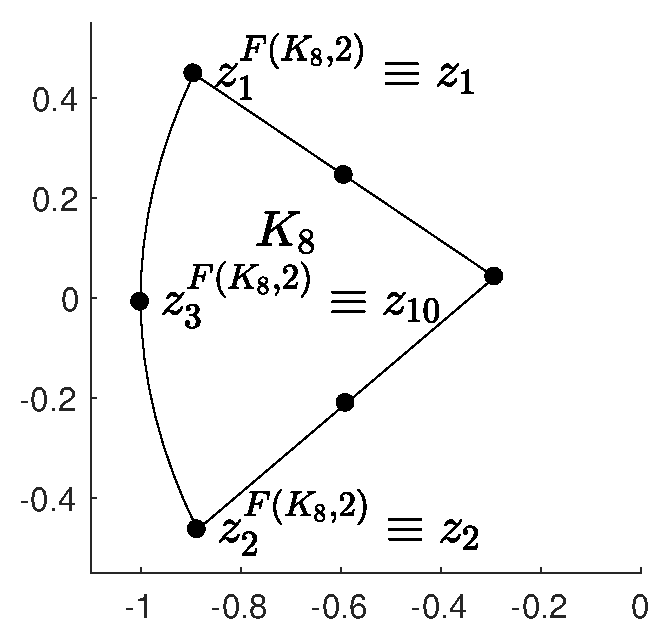
\includegraphics[width=0.33\textwidth]{isomap_p2_phy_edge}
    %\label{fig:fe_impl_isomap_p1_phy}
  }
  \caption{$\PP^2$ geometry mapping for a facet. \label{fig:fe_impl_isomap_face_p2}}
\end{figure}
Our geometry mapping for the facet, $\calG^F: \tilde I \to F$, is given by
\begin{equation}
  x = \calG^F(\tilde s) \equiv \sum_{\alpha=1}^{n_s^F} z^F_\alpha \tilde \chi_{\alpha}(\tilde s),
  \label{eq:fe_iso_map_face}
\end{equation}
where $z^F_\alpha \in \RR^{d \equiv 2}$ is the coordinate of the $\alpha$-th node of the physical facet $F \subset \RR^{d \equiv 2}$, $\chi_{\alpha} \in \PP^{p \equiv 2}(\tilde I)$ is the Lagrange shape function associated with the $\alpha$-th node of the reference line segment $\tilde I \subset \RR^1$, and $n_s^F = 3$ for the $\PP^2(\tilde I)$ space.  Note that the input is $\tilde s \in \tilde I \subset \RR^{d-1 \equiv 1}$ while the output is $x \in F \subset \RR^{d \equiv 2}$.  Similar to the geometry mapping~\eqref{eq:fe_iso_map} for the element, the geometry mapping~\eqref{eq:fe_iso_map_face} is a polynomial map of degree $p$ that maps the interpolation nodes $\{\tilde z_i\}$ of the reference line segment $\tilde I$ to the associated nodes $\{z_i^{F}\}$ of the physical facet $F$.

We can differentiate~\eqref{eq:fe_iso_map_face} to obtain the Jacobian, $J^F: \tilde I \to \RR^{d \times (d-1)}$, given by
\begin{equation*}
  J^F_{ij}(\tilde s)
  \equiv
  \left. \pp{x_i}{\tilde s_j} \right|_{\tilde s}
  =
  \left. \pp{\calG^F}{\tilde s_j} \right|_{\tilde s}
  =
  \sum_{\alpha = 1}^{n_s^F} z^F_\alpha \left. \pp{\tilde \phi_\alpha}{\tilde s_j} \right|_{\tilde s},
  \quad i = 1,\dots,d, \ j = 1,\dots,d-1.
\end{equation*}
The Jacobian is rectangular because the mapping is from $\RR^{d-1}$ to $\RR^d$. The Jacobian $J^F(\tilde s)$ characterizes how an infinitesimal line segment $d\tilde l$ at $\tilde s \in \tilde I$ maps to an infinitesimal line segment $dl$ at $s \in F$: $dl = J^F(\tilde s) d\tilde l$.

The physical length $ds$ is related to the reference length $d\tilde s$ by the relationship
\begin{equation*}
  ds = |J^F(\tilde s)|d\tilde s,
\end{equation*}
where, in two dimensions, 
\begin{equation*}
  |J^F(\tilde s)| \equiv \sqrt{J^F_{11}(\tilde s)^2 + J^F_{21}(\tilde s)^2}.
\end{equation*}
Analogously to the determinant condition $|J(\tilde x)| > 0$ $\forall \tilde x \in \tilde K$ for the element mapping, a facet mapping is valid if and only if
\begin{equation*}
  |J^F(\tilde s)| > 0 \quad \forall \tilde s \in \tilde I.
\end{equation*}
This condition is automatically satisfied if $|J^K(\tilde x)| >0$ $\forall \tilde x \in \bar{\tilde K}$ for the element $K$ associated with the facet $F$.

The evaluation of forms associated with a boundary value problem sometimes also require the evaluation of the \emph{unit outward-pointing normal vector}. In two dimension, the normal vector is given by
\begin{equation*}
  n^F(\tilde s) = \frac{1}{|J^F(\tilde s)|} \bmat{c} -J^F_{21}(\tilde s) \\ J^F_{11}(\tilde s) \emat .
\end{equation*}
This definition of the normal vector is for our counter-clockwise convention for the facet orientation; the sign needs to be reversed if the clockwise convection is used for the facet orientation.

\section{Numerical quadrature}
\label{sec:fe_quad}
\subsection{Motivation}
The evaluation of bilinear and linear forms that appear in the weak form of boundary value problems requires integration of functions. 
%% The entries of the element stiffness matrix $\hat A^K \in \RR^{n_s \times n_s}$ can be expressed as an integral over the reference element $\tilde K$:
%% \begin{align*}
%%   \hat A^K_{\alpha\beta}
%%   &\equiv \int_{K} \left. \pp{\phi_\alpha^K}{x_i} \right|_{x} a_{ij}(x) \left. \pp{\phi_\beta^K}{x_j} \right|_x dx
%%   \\
%%   &= \int_{\tilde K} \left. \pp{\phi_\alpha^K}{x_i} \right|_{x(\tilde x)} a_{ij}(x(\tilde x)) \left. \pp{\phi_\beta^K}{x_j} \right|_{x(\tilde x)} |J(\tilde x)| d\tilde x , \quad \alpha,\beta = 1,\dots,n_s.
%% \end{align*}
%% So far in this lecture we have introduced the means to evaluate all the terms that appear in the integrand --- $\left. \pp{\phi_\alpha^K}{x_i} \right|_{x(\tilde x)}$, $a_{ij}(x(\tilde x))$, and $|J(\tilde x)|$.  The last ingredient we need is a means to evaluate the integral over $\tilde K$ from a finite evaluation of the integrand.
This integration is performed by \emph{numerical quadrature} (or just \emph{quadrature}).  Specifically, our quadrature problem is as follows: given a reference element $\tilde K$ and a function $f: \tilde K \to \RR$, estimate the integral
\begin{equation*}
  I \equiv \int_{\tilde K} f(\tilde x) d \tilde x
\end{equation*}
by
\begin{equation*}
  Q \equiv \sum_{q=1}^{n_q} \tilde \rho_q f(\tilde \xi_q),
\end{equation*}
where $\{\tilde \xi_q \in \tilde K \}_{q=1}^{n_q}$ is a set of \emph{quadrature points} and $\{\tilde \rho_q \in \RR \}_{q=1}^{n_q}$ is the associated set of \emph{quadrature weights}. 

\subsection{Gauss quadrature in $\RR^1$}
\label{sec:fe_quad_1d}
We first consider a one-dimensional quadrature for a unit line segment $\tilde I \equiv (0,1) \subset \RR^1$.  (Note: one-dimensional quadrature rules are more often defined for the line segment $(-1,1)$; in this lecture we define them for $(0,1)$ to be consistent with our definition of a unit line segment.)  While there are many different families of one-dimensional quadrature rules, we focus on arguably the most efficient quadrature rule: the Gauss quadrature.

The $n_q$-point Gauss quadrature rule is defined by quadrature points $\{\tilde \xi_q \in \tilde I \}_{q=1}^{n_q}$ and quadrature weights $\{ \tilde \rho_q \in \tilde I \}_{q=1}^{n_q}$ such that the rule integrates exactly polynomials of degrees up to and including $2n_q - 1$: i.e.,
\begin{equation}
  \int_{\tilde I} f(\tilde x) d\tilde x = \sum_{q=1}^{n_q} \tilde \rho_q f(\tilde \xi_q) \quad \forall f \in \PP^{2n_q-1}(\tilde I).
  \label{eq:fe_impl_gauss_cond}
\end{equation}
Our intuition might suggest the existence of such a quadrature rule, as the polynomials of degree $2n_q-1$ have $2n_q$ degrees of freedom and the $n_q$-point quadrature rule also has $2n_q$ degrees of freedom --- $n_q$ point locations and $n_q$ weigh values.


We can show the existence of a $n_q$-point quadrature rule that exactly integrates polynomials of degree $2n_q-1$ in a constructive manner.  To this end, we use the scaled Legendre polynomials $\{ \tilde \psi_i \}$ over $\tilde I$ defined in Definition~\ref{def:fe_legendre_poly}. We first choose the quadrature points $\{ \tilde \xi_q \}_{q=1}^{n_q}$ as the roots of the degree $n_q$ Legendre polynomial:
\begin{equation}
  \tilde \psi_{n_q}(\tilde \xi_q) = 0, \quad q = 1,\dots,n_q.
  \label{eq:fe_impl_gauss_points}
\end{equation}
We then choose the quadrature weights $\{\tilde \rho_q \}_{q=1}^{n_q}$ to satisfy the following linear equation:
\begin{equation}
  \bmat{ccc}
  \tilde \psi_0(\tilde \xi_1) & \dots & \tilde \psi_0(\tilde \xi_{n_q}) \\
  \vdots & \ddots & \vdots \\
  \tilde \psi_{n_q-1}(\tilde \xi_1) & \dots & \tilde \psi_{n_q-1}(\tilde \xi_{n_q}) 
  \emat
  \bmat{c}
  \tilde \rho_1 \\ \vdots \\ \tilde \rho_{n_q}
  \emat
  =
  \bmat{c}
  \int_{\tilde I} \tilde \psi_0(\tilde x) d\tilde x \\
  \vdots \\
  \int_{\tilde I} \tilde \psi_{n_q-1}(\tilde x) d\tilde x
  \emat .
  \label{eq:fe_impl_gauss_weights}
\end{equation}
%This linear system is well-posed.
%The linear system is well-posed because the Legendre polynomials $\{ \tilde \psi_i \}_{i=0}^{n_q-1}$ are linearly independent and the $n_q$ quadrature points are distinct.

We wish to show the conditions~\eqref{eq:fe_impl_gauss_points}~and~\eqref{eq:fe_impl_gauss_weights} yield a quadrature rule that integrates exactly polynomials of degree $2n_q-1$. To begin, we introduces a basis $\{p_i\}_{i=0}^{2n_q-1}$ for $\PP^{2n_q-1}(\tilde I)$ such that $\forall \tilde x \in \tilde I$
\begin{align*}
  p_0(\tilde x) &= \tilde \psi_0(\tilde x) = 1, &
  p_1(\tilde x) &= \tilde \psi_1(\tilde x), &
  &\dots, &
  p_{n_q-1}(\tilde x) &= \tilde \psi_{n_q-1}(\tilde x) \\
  p_{n_q}(\tilde x) &= \tilde \psi_{n_q}(\tilde x) \tilde \psi_0(\tilde x), & 
  p_{n_q+1}(\tilde x) &= \tilde \psi_{n_q}(\tilde x) \tilde \psi_1(\tilde x), &  
  &\dots, &
  p_{2n_q-1}(\tilde x) &= \tilde \psi_{n_q}(\tilde x) \tilde \psi_{n_q-1}(\tilde x) .
%  p_0(x) &= \tilde \psi_0(x) = 1 \\
%  p_1(x) &= \tilde \psi_1(x) \\
%  &\vdots \\
%  p_{n_q-1}(x) &= \tilde \psi_{n_q-1}(x) \\
%  p_{n_q}(x) &= \tilde \psi_{n_q}(x) \tilde \psi_0(x) \\
%  p_{n_q+1}(x) &= \tilde \psi_{n_q}(x) \tilde \psi_1(x) \\
%  &\vdots \\
%  p_{2n_q-1}(x) &= \tilde \psi_{n_q}(x) \tilde \psi_{n_q-1}(x) 
\end{align*}
The polynomials $\{ p_i \}_{i=0}^{2n_q - 1}$ is a basis for $\PP^{2n_q - 1}(\tilde I)$; the set spans $\PP^{2n_q-1}(\tilde I)$ and is linearly independent because $p_i$ is a polynomial of degree (exactly) $i$ for $i = 0,\dots,2 n_q - 1$.
We now wish to confirm that
\begin{equation}
  \int_{\tilde I} p_i(\tilde x) dx = \sum_{q=1}^{n_q} \tilde \rho_q p_i(\tilde \xi_q), \quad \forall i = 0,\dots,2 n_q - 1,
  \label{eq:fe_impl_gauss_cond_2}
\end{equation}
which is equivalent to the original condition~\eqref{eq:fe_impl_gauss_cond}. We first readily confirm that the first $n_q$ basis functions, $\{p_i\}_{i=0}^{n_q} \equiv \{ \tilde \psi_i \}_{i=0}^{n_q}$, are integrated exactly because our weights $\{ \tilde \rho_q \}_{q=1}^{n_q}$ are chosen to integrate the functions in condition~\eqref{eq:fe_impl_gauss_weights}. 
To prove that the next $n_q$ basis functions, $\{ p_i \}_{i=n_q}^{2n_q-1}$ are integrated exactly, we observe that the left-hand side of~\ref{eq:fe_impl_gauss_cond_2} for $i = n_q,\dots,2_{n_q}-1$ yields 
\begin{equation*}
  (\text{LHS})
  = \int_{\tilde I} p_{p+j}(\tilde x) d \tilde x
  = \int_{\tilde I} \tilde \psi_{n_q}(\tilde x) \tilde \psi_{j}(\tilde x) d \tilde x
  = 0, \quad j = 0,\dots,n_q,
\end{equation*}
since the Legendre polynomials are orthogonal in $L^2(\tilde I)$. On the other hand, the right-hand side of~\ref{eq:fe_impl_gauss_cond_2} for $i = n_q,\dots,2_{n_q}-1$ yields
\begin{equation*}
  (\text{RHS})
  = \sum_{q=1}^{n_q} \tilde \rho_q p_{p+j}(\tilde \xi_q)
  = \sum_{q=1}^{n_q} \tilde \rho_q \tilde \psi_{n_q}(\tilde \xi_q) \tilde \psi_{j}(\tilde \xi_q)
  = 0, \quad j = 0,\dots,n_q,
\end{equation*}
since $\{\tilde \xi_q\}_{q=1}^{n_q}$ are the roots of $\tilde \psi_{n_q}$ by~\eqref{eq:fe_impl_gauss_points}. In summary, the exact integration condition~\ref{eq:fe_impl_gauss_cond_2} are satisfied (i) for $i = 0,\dots,n_q-1$ because of the choice of the weights $\{\tilde \rho_q\}_{q=1}^{n_q}$ ~\eqref{eq:fe_impl_gauss_weights} and (ii) for $i = n_q, \dots, 2 n_q-1$ because of the choice of the points $\{\tilde \xi_q\}_{q=1}^{n_q}$ by~\eqref{eq:fe_impl_gauss_points}.

Table~\ref{tb:fe_impl_gauss} shows the Gauss quadrature rules for $n_q = 1,\dots,4$.  As visualized in Figure~\ref{fig:fe_impl_gauss_points}, the quadrature points are clustered towards the endpoints.
\begin{figure}
  \centering
  \subfigure[$p = 1$]{
    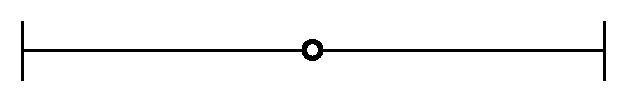
\includegraphics[width=0.45\textwidth]{quad_1d_p1}
  }
  \subfigure[$p = 3$]{
    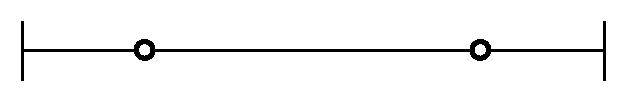
\includegraphics[width=0.45\textwidth]{quad_1d_p3}
  }
  \subfigure[$p = 5$]{
    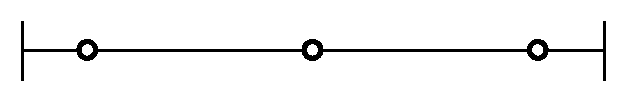
\includegraphics[width=0.45\textwidth]{quad_1d_p5}
  }
  \subfigure[$p = 7$]{
    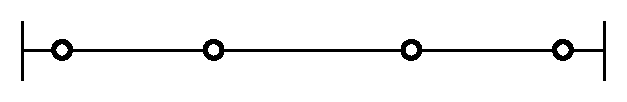
\includegraphics[width=0.45\textwidth]{quad_1d_p7}
  }
  \caption{Gauss quadrature points for $(0,1)$. \label{fig:fe_impl_gauss_points}}
\end{figure}

\begin{table}
  \centering
  \begin{tabular}{cccc}
    $p$ & $n_q$ & $\tilde \xi$ & $\tilde \rho$ \\
    \hline
    $1$ & $1$ & $0.500000000000000$ & $1.000000000000000$ \\
    \hline
    $3$ & $2$ & $0.211324865405187$ & $0.500000000000000$ \\ 
    & & $0.788675134594813$ & $0.500000000000000$ \\
    \hline
    $5$ & $3$ & $0.112701665379258$ & $0.277777777777778$ \\ 
     & & $0.500000000000000$ & $0.444444444444444$ \\ 
     & & $0.887298334620742$ & $0.277777777777778$ \\
    \hline
    $7$ & $4$ & $0.069431844202974$ & $0.173927422568727$ \\ 
    & & $0.330009478207572$ & $0.326072577431273$ \\ 
    & & $0.669990521792428$ & $0.326072577431273$ \\ 
    & & $0.930568155797026$ & $0.173927422568727$ 
  \end{tabular}
  \caption{Gauss quadrature rules on $\tilde I$ for $p = 1$ to $7$ polynomials. \label{tb:fe_impl_gauss}}
\end{table}

\subsection{Numerical quadrature in $\RR^d$}
\label{sec:fe_quad_nd}
Similarly to the Gauss quadrature in $\RR^1$, there also exists efficient quadrature rules for integration of domains in $\RR^{d > 1}$.  If the domain is a unit square $[0,1]^2 \equiv \tilde I^2 \subset \RR^2$ or a unit cube $[0,1]^3 \equiv \tilde I^3 \subset \RR^3$, then we can obtain the associated quadrature rule by the tensor-product of the one-dimensional Gauss rules; for example, for $[0,1]^2$, 
\begin{equation*}
  \int_{\tilde x_2=0}^1 \int_{\tilde x_1=0}^1 f(\tilde x_1,\tilde x_2) d\tilde x_1 d\tilde x_2
  \approx \sum_{i_2 = 1}^{n_q^{\rm 1d}} \sum_{i_1 = 1}^{n_q^{\rm 1d}} \tilde \rho_{i_2}^{\rm 1d} \tilde \rho_{i_1}^{\rm 1d} f(\tilde \xi_1^{\rm 1d}, \tilde \xi_2^{\rm 1d}).
\end{equation*}
These rules maximizes the degree of tensor-product polynomials integrated exactly for a given number of quadrature points.

For a domain in $\RR^{d < 1}$, that does not result from a tensor-product of a one-dimensional domain, the ``optimal'' quadrature rules are much more difficult to identify.  In fact, the optimal rules for (say) a triangle is not as universally standardized as that for a square. Table~\ref{tb:fe_impl_integ_gauss2} shows examples of efficient quadrature rule for our unit right triangle, which integrates exactly polynomials of degree $p$.  Figure~\ref{fig:fe_impl_integ_gauss2} visualizes the quadrature points.  Similarly to the one-dimensional Gauss rule, the quadrature points are clustered towards the edge of the triangular domain.


\begin{table}
  \centering
  \begin{tabular}{ccccc}
    $p$ & $n_q$ & $\tilde \xi_1$ & $\tilde \xi_2$ & $\tilde \rho$ \\
    \hline
    $1$ & $1$ & $0.333333333333333$ & $0.333333333333333$ & $0.500000000000000$ \\
    \hline
    $2$ & $3$ & $0.166666666666667$ & $0.166666666666667$ & $0.166666666666667$ \\ 
    & & $0.666666666666667$ & $0.166666666666667$ & $0.166666666666667$ \\ 
    & & $0.166666666666667$ & $0.666666666666667$ & $0.166666666666667$ \\ 
    \hline
    $4$ & $6$ & $0.091576213509771$ & $0.091576213509771$ & $0.054975871827661$ \\ 
    & & $0.816847572980459$ & $0.091576213509771$ & $0.054975871827661$ \\ 
    & & $0.091576213509771$ & $0.816847572980459$ & $0.054975871827661$ \\ 
    & & $0.445948490915965$ & $0.445948490915965$ & $0.111690794839006$ \\
    & & $0.108103018168070$ & $0.445948490915965$ & $0.111690794839006$ \\ 
    & & $0.445948490915965$ & $0.108103018168070$ & $0.111690794839006$ \\ 
  \end{tabular}
  \caption{Efficient quadrature rules on $\tilde T$ for $p = 1$ to $4$ polynomials.}
  \label{tb:fe_impl_integ_gauss2}
\end{table}

\begin{figure}
  \centering
  \subfigure[$p = 1$]{
    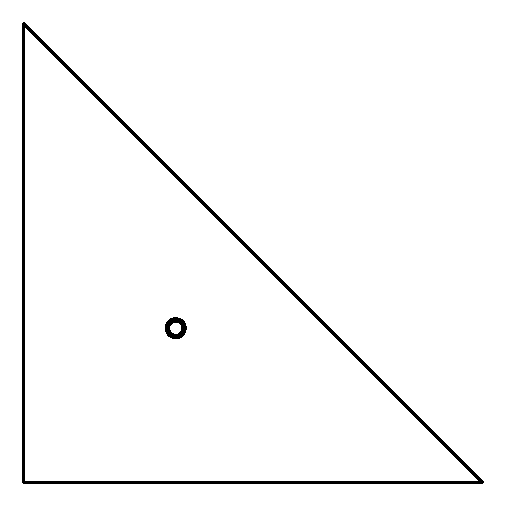
\includegraphics[width=0.23\textwidth]{quad_2d_p1}
  }
  \subfigure[$p = 2$]{
    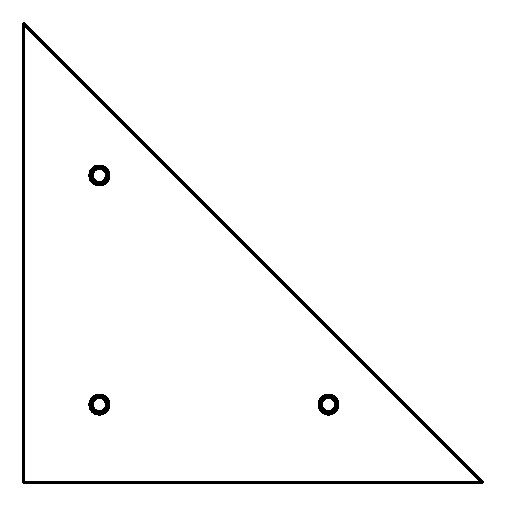
\includegraphics[width=0.23\textwidth]{quad_2d_p2}
  } 
  \subfigure[$p = 4$]{
    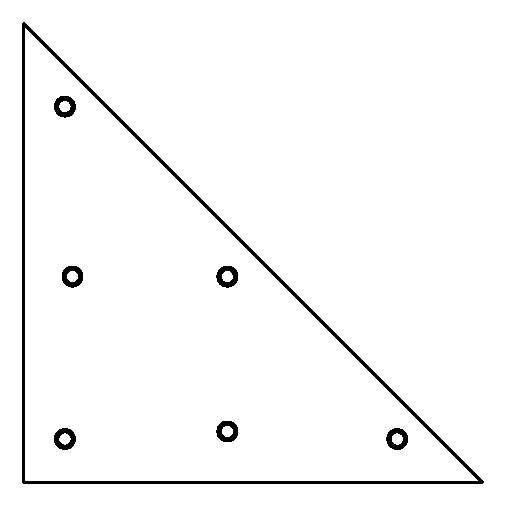
\includegraphics[width=0.23\textwidth]{quad_2d_p4}
  } 
  \subfigure[$p = 5$]{
    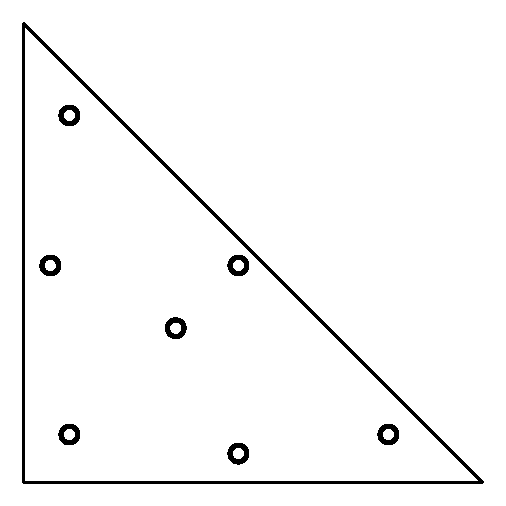
\includegraphics[width=0.23\textwidth]{quad_2d_p5}
  }
  \subfigure[$p = 6$]{
    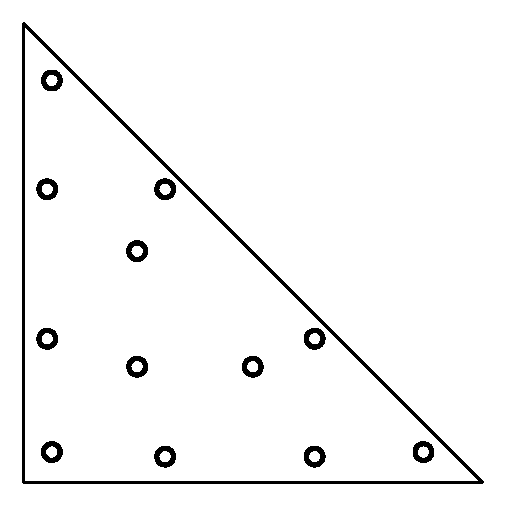
\includegraphics[width=0.23\textwidth]{quad_2d_p6}
  }
  \subfigure[$p = 7$]{
    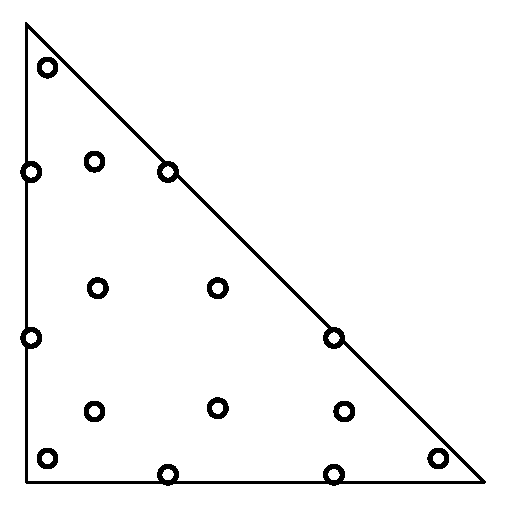
\includegraphics[width=0.23\textwidth]{quad_2d_p7}
  }
  \caption{Numerical quadrature points for the reference triangle.}
  \label{fig:fe_impl_integ_gauss2}
\end{figure}

\section{Assembly}
\label{sec:fe_assembly}
\subsection{Local stiffness matrices and vectors}
We now put together the techniques we have learned in this lecture to evaluate local stiffness matrices and load vectors.  To provide a concrete example, in this section we consider $\calV \equiv H^1(\Omega)$, a bilinear form $a: \calV \times \calV \to \RR$ such that
\begin{equation}
  a(w,v) \equiv \int_\Omega \nabla v \cdot a \nabla w dx , \quad \forall w,v \in \calV,
  \label{eq:fe_impl_model_a}
\end{equation}
for $a: \Omega \to \RR^{d \times d}$ the diffusion tensor field, and a linear form $\ell: \calV \to \RR$ such that
\begin{equation}
  \ell(v) \equiv \int_\Omega v f dx \quad \forall v \in \calV,
  \label{eq:fe_impl_model_ell}
\end{equation}
for $f: \Omega \to \RR$ the source function. Our approximation space is given by
\begin{equation}
  \calV_h \equiv \{ v \in \calV \ | \ v|_K \circ \calG^K \in \PP^p(\tilde K), \ \forall K \in \calT_h \},
  \label{eq:fe_impl_loc_vh}
\end{equation}
where $\calG^K: \tilde K \to K$ is a $\PP^p$ geometry mapping. The number of shape functions per element is denoted by $n_s$.

We first consider the evaluation of the \emph{local load vector} $\hat f^K \in \RR^{n_s}$ such that
\begin{equation*}
  \hat f^K_\alpha \equiv \ell(\phi^K_\alpha) \quad \forall \alpha = 1,\dots,n_s.
\end{equation*}
For our model linear form~\eqref{eq:fe_impl_model_ell}, the local load vector is given by
\begin{equation*}
  \hat f^K_\alpha
  \equiv \ell(\phi^K_\alpha) \equiv \int_K \phi^K_\alpha(x) f(x) dx , \quad \alpha = 1,\dots, n_s.
\end{equation*}
We now change the integration domain from the physical domain $K$ to the reference domain $\tilde K$; this is in preparation for the application of the numerical quadrature on the reference domain.  We employ (i) the geometry mapping for the argument of $f$, $x = \calG^K(\tilde x)$, (ii) the relationship between the reference and physical shape functions, $\phi^K_\alpha(x \equiv \calG^K(\tilde x)) = \tilde \phi_\alpha(\tilde x)$, and (iii) the area transformation $dx = |J^K(\tilde x)| d \tilde x$, where $|J^K|$ is the determinant of the Jacobian of the geometry mapping, to obtain 
\begin{equation}
  \hat f^K_\alpha
  = \int_{\tilde K} \phi_\alpha(\tilde x) f(\calG^K(\tilde x)) |J(\tilde x)| d \tilde x .
  \label{eq:fe_impl_loc_vec_2}
\end{equation}
We finally apply a $n_q$-point numerical quadrature to ``evaluate'' the integral:
\begin{equation*}
    \hat f^K_\alpha \
    \text{``}\hspace{-0.2em}=\hspace{-0.2em}\text{''}
    \ \sum_{q=1}^{n_q} \tilde \rho_q \tilde \phi_\alpha(\tilde \xi_q) f(\calG^K(\tilde \xi_q)) |J(\tilde \xi_q)| .
\end{equation*}
Here, we put the equality in quotes because the evaluation is exact only if the integrand is a polynomial that can be integrated exactly using the quadrature rule.  Otherwise, the use of the numerical quadrature results in an \emph{approximation} rather than an \emph{evaluation}. In any event, we can readily evaluate the quantities in the summand using the techniques discussed in the previous sections. We here make a listing for a reference: 
%\begin{itemize}
%\item
(i) Quadrature rule $\{\tilde \xi_q, \tilde \rho_q\}_{q=1}^{n_q}$ was discussed in Sections~\ref{sec:fe_quad};
(ii) The evaluation of quantities associated with geometry mapping, $\calG^K$ and $J^K$, was discussed in Sections~\ref{sec:fe_iso_map};
(iii) The evaluation of reference shape functions $\{\tilde \phi_\alpha \}_{\alpha=1}^{n_s}$ was discussed in Section~\ref{sec:fe_ref_elem}.
%\end{itemize}
%We hence can evaluate (or approximate) the local load vector $\hat f^K \in \RR^{n_s}$.

We now consider the evaluation of the \emph{local stiffness matrix} $\hat A^K \in \RR^{n_s \times n_s}$ such that
\begin{equation*}
  \hat A^K_{\alpha,\beta} \equiv a(\phi^K_\beta,\phi^K_\alpha) \quad \forall \alpha,\beta = 1,\dots,n_s.
\end{equation*}
For our model bilinear form~\eqref{eq:fe_impl_model_a}, the local stiffness matrix is given by
\begin{equation*}
  \hat A^K_{\alpha,\beta}
  \equiv
  a(\phi^K_\beta,\phi^K_\alpha) = \int_K \nabla \phi^K_\alpha(x) \cdot a(x) \nabla \phi^K_\beta(x) dx , \quad \alpha,\beta = 1,\dots,n_s.
\end{equation*}
Following the same procedure we used for the evaluation (or approximation) of the local load vector $\hat f_h^K \in \RR^{n_s}$, we now change the integration domain from the physical domain $K$ to the reference domain $\tilde K$.  We employ (i) the geometry mapping for the argument of $a$, $x = \calG^K(\tilde x)$, (ii) the relationship between the derivatives of the reference and physical shape functions, $\nabla \phi^K(x = \calG(\tilde x)) = J^K(\tilde x)^{-T} \tilde \nabla \tilde \phi(\tilde x)$, and (iii) the area transformation $dx = |J^K(\tilde x)| d \tilde x$, where $|J^K|$ is the determinant of the Jacobian of the geometry mapping, to obtain
\begin{equation}
  \hat A^K_{\alpha,\beta}
  =
  \int_{\tilde K} ((J^K)^{-T}(\tilde x) \tilde \nabla \tilde \phi(\tilde x))
  \cdot a(\calG^K(\tilde x)) (J^K(\tilde x)^{-T}) \tilde \nabla \tilde \phi(\tilde x)
  |J(\tilde x)| d\tilde x
  \label{eq:fe_impl_loc_mat_2}
\end{equation}
We finally apply a $n_q$-point numerical quadrature to ``evaluate'' the integral:
\begin{equation*}
  \hat A^K_{\alpha,\beta}
  \text{``}\hspace{-0.2em}=\hspace{-0.2em}\text{''}
  \sum_{q=1}^{n_q} \tilde \rho_q
   (J^K(\tilde \xi_q)^{-T} \tilde \nabla \tilde \phi(\tilde \xi_q))
  \cdot a(\calG^K(\tilde \xi_q)) J^K(\tilde \xi_q)^{-T} \tilde \nabla \tilde \phi(\tilde \xi_q)
  |J^K(\tilde \xi_q)|.
\end{equation*}
Again, we put the equality in quotes because the evaluation is exact only if the integrand is a polynomial that can be integrated exactly using the quadrature rule.  In particular, in the presence of a curved element, the integrand is almost always non-polynomial because the inverse Jacobian is non-polynomial. The techniques used to evaluate the element stiffness matrix are almost identical to those used to evaluate the element load vector, except this time we also employ the technique to evaluate the derivative of the physical shape functions discussed in Section~\ref{sec:fe_phy_shape}. If the bilinear form contains other terms, such as a convection term of the form $\int_{\Omega} v b \cdot \nabla w dx$ or a reaction term of the form $\int_\Omega c v w dx$, they can also be evaluated in a similar manner.


We make one note about the expressions for the local load vector and stiffness matrix.  In literature, the expressions~\eqref{eq:fe_impl_loc_vec_2} and \eqref{eq:fe_impl_loc_mat_2} are sometimes restated as
\begin{align*}
  \hat f^K_\alpha
  &=
  \int_{\tilde K} \phi_\alpha(\tilde x) \underbrace{ f(\calG^K(\tilde x)) |J^K(\tilde x)| }_{\equiv f^{\rm trans}(\tilde x)}d \tilde x, \\
  \hat A^K_{\alpha,\beta}
  &=
  \int_{\tilde K} \tilde \nabla \tilde \phi(\tilde x)
  \cdot  \underbrace{ (J^K(\tilde x)^{-1} a(\calG^K(\tilde x)) J^K(\tilde x)^{-T} |J^K(\tilde x)| }_{\equiv  a^{\rm trans}(\tilde x)}\tilde \nabla \tilde \phi(\tilde x)  d\tilde x,
\end{align*}
where $f^{\rm trans}: \tilde K \to \RR$  and $a^{\rm trans}:\tilde K \to \RR^{d \times d}$ are the transformed coefficients for the reference domain $\tilde K$. Note that the difference lies only in the interpretation; the local load vectors and stiffness matrices for both formulations are mathematically identical.

\subsection{Local stiffness matrix and vectors: facet terms}
We now consider evaluation of a load vector that requires integration on a boundary and, in turn, on a facet.  Again to provide a concrete example, in this section we consider $\calV \equiv H^1(\Omega)$, a linear form $\ell: \calV \to \RR$ such that
\begin{equation}
  \ell(v) \equiv \int_{\Gamma_N} v g dx \quad \forall v \in \calV,
  \label{eq:fe_impl_model_g}
\end{equation}
for $g: \Gamma_N \to \RR$ the Neumann source function. Our approximation space $\calV_h$ is as defined in~\eqref{eq:fe_impl_loc_vh}.  The number of shape fucntions per element is denoted by $n_s$, and the number of shape functions on a facet of the element is denoted by $n_s^F$.  (We only consider the load vector, and not the stiffness matrix, as the evaluation procedures are essentially the same.)

By way of preliminaries, we first provide a triangular for the boundary $\Gamma_N$.  The boundary triangulation
\begin{equation*}
  \calT_h^{\Gamma_N} \equiv \{ F_i \}_{i=1}^{n_f}
\end{equation*}
is a set of $n_f$ non-overlapping facets that cover the boundary $\Gamma_N$: (i) $F_i \cap F_j = \emptyset$, $i \neq j$, and (ii) $\cup_{i=1}^{n_f} \bar F_i = \bar \Gamma_N$.  We assume that the facet triangulation $\calT_h^{\Gamma_N}$ is compatible with the domain triangulation $\calT_h \equiv \{ K_i \}_{i=1}^{n_e}$ in the sense that each $F_i \in \calT_h^{\Gamma_N}$ is a facet of a unique element.  Given this compatibility condition, we introduce two mappings:
\begin{itemize}
\item[1.] $\theta_{F\text{-}K}: \{ 1,\dots,n_f\} \to \{1,\dots,n_e\}$. Mapping from a physical facet number to the element to which the facet belongs.
\item[2.] $\theta_{F\text{-}\tilde F}: \{1,\dots,n_f\} \to \{1,2,3\}$. Mapping from a physical facet number to the local facet index.
\end{itemize}
These two mappings combined implies that a physical facet $F$ is the $i = \theta_{F\text{-}\tilde F}(K)$-th facet of the element $K_{j \equiv \theta_{F\text{-}K}(F)}$.

To evaluate the local load vector $\tilde f^K \in \RR^{n_s}$, we appeal to the fact that the restriction of an element shape function $\phi^K$ in $\RR^d$ to a facet $F$ is a shape function in $\RR^{d-1}$:
\begin{equation*}
  \phi^K_{\alpha}|_{F} = \chi_\gamma^F, \quad \forall \gamma =1,\dots,n_s^F,
\end{equation*}
for  $K = \theta_{F\text{-}K}(F)$, $\alpha = \theta_{\tilde F\text{-}n}(i,\gamma)$, and $i = \theta_{F\text{-}\tilde F}(F)$.  We recall that the mapping $\theta_{\tilde F\text{-}n}$ is the mapping from facet nodes to element nodes introduced in  Sections~\ref{sec:fe_lin_tri}~and~\ref{sec:fe_p2_tri}; $\alpha = \theta_{\tilde F\text{-}(n)}(i,\gamma)$ is the element node that corresponds to the $\gamma$-th facet node of the $i$-th facet.  Our approach is hence to evaluate the boundary integral using the facet shape functions $\{\chi^F_\gamma\}_{\gamma =1}^{n_s^F}$ and then to map the appropriate integrals to the element integral.  Specifically, we note that if the linear form $\ell(\cdot)$ only involves integration on a boundary,
\begin{equation}
  \ell(\phi^{K}_{\alpha}|_F) = \ell(\chi_\gamma^{F}), \quad \forall \gamma = 1,\dots,n_s^F,
  \label{eq:fe_impl_chiK_to_phiK}
\end{equation}
for  $K = \theta_{F\text{-}K}(F)$, $\alpha = \theta_{\tilde F\text{-}n}(i,\gamma)$, and $i = \theta_{F\text{-}\tilde F}(F)$.  For our model linear form~\eqref{eq:fe_impl_model_g} the evaluation of the integral for $\{\chi_\gamma^F\}_{\gamma=1}^{n_s^F}$ yields
%To evaluate the local load vector $\tilde f^K \in \RR^{n_s}$, we appeal to the fact that for the shape functions $\{\phi^K_{\alpha}\}_{\alpha=1}^{n_s}$ in $\RR^d$ their restrictions to the facets are given by the shape functions $\{\chi^F_\gamma\}_{\gamma=1}^{n_s^F}$ in $\RR^{d-1}$, as discussed in Sections~\ref{sec:fe_lin_tri}~and~\ref{sec:fe_p2_tri}.  Specifically, we appeal to the map
%\begin{equation*}
%  \ell(\phi^{K(F)}_{\alpha = \theta_{\rm e-f}(i,\gamma)}|_{F}) = \ell(\chi_\gamma^{F}), \quad \forall \gamma = 1,\dots,n_s^F,
%\end{equation*}
%where $K(F)$ is element associated with the (boundary) facet $F$, $i$ is the local facet number for $F$ within $K$, and $\alpha = \theta_{\rm e-f}(i,\gamma)$ is the Lagrange node of the element $K$ that corresponds to the $\gamma$-th Lagrange node of the facet $F$.  We now evaluate our model linear form~\eqref{eq:fe_impl_model_g} for $\{\chi_\gamma^F\}_{\gamma=1}^{n_s^F}$, 
\begin{equation*}
  \hat g^F_\gamma \equiv \ell(\chi_\gamma^F) = \int_{F} \chi^F_\gamma(s) g(s) ds, \quad \gamma = 1,\dots,n_s^F.
\end{equation*}
To evaluate (or approximate) the integral, we change the integration domain from the physical facet $F$ to the reference line segment $\tilde I$.  We employ (i) the facet geometric mapping for the argument of $g$, $s \equiv \calG^F(\tilde s)$, (ii) the relationship between the reference and physical shape functions, $\tilde \chi^F_\gamma(s \equiv \calG^F(\tilde s)) = \tilde \chi(\tilde s)$, and (iii) the length transformation $ds = |J^F(\tilde s)|d \tilde s$, to obtain
\begin{equation*}
  \hat g^F_\gamma = \int_{\tilde I} \tilde \chi_\gamma(\tilde s) g(\calG^F(\tilde s)) |J^F(\tilde s)| d \tilde s.
\end{equation*}
We then apply a $n_q$-point numerical quadrature defined by $\{ \tilde \xi_q, \tilde \rho_q \}_{q=1}^{n_q}$ to ``evaluate'' the integral:
\begin{equation*}
  \hat g^F_\gamma
  \text{``}\hspace{-0.2em}=\hspace{-0.2em}\text{''}
  \sum_{q=1}^{n_q} \tilde \rho_q \tilde \chi_\gamma(\tilde \xi_q) g(\calG^F(\tilde \xi_q)) |J^F(\tilde \xi_q)| .
\end{equation*}
We finally map the vector $\hat g^F \in \RR^{n_s^F}$ to $\hat f^K \in \RR^{n_s}$ according to
\begin{equation*}
  \hat f^{K}_{\alpha} = \hat g^F_\gamma, \quad \forall \gamma = 1,\dots,n_s^F,
\end{equation*}
for  $K = \theta_{F\text{-}K}(F)$, $\alpha = \theta_{\tilde F\text{-}n}(i,\gamma)$, and $i = \theta_{F\text{-}\tilde F}(F)$.  This mapping appeals to the relationship~\eqref{eq:fe_impl_chiK_to_phiK}.



\subsection{Global matrix and vector assembly}
We have so far introduced technical ingredients required to assemble, for any $K \in \calT_h$, 
and the local load vector $\hat f^K \in \RR^{n_s}$ such that
\begin{equation*}
  \hat f^K_\alpha = \ell(\phi^K_\alpha) \quad \forall \alpha = 1,\dots,n_s,
\end{equation*}
and a local stiffness matrix $\hat A^K \in \RR^{n_s \times n_s}$ such that
\begin{equation*}
  \hat A^K_{\alpha,\beta} = a(\phi^K_\beta,\phi^K_\alpha) \quad \forall \alpha, \beta = 1,\dots,n_s.
\end{equation*}
We now wish to assemble the local stiffness matrices and vectors construct the (global) stiffness matrix and vector.

To this end, we employ the element-to-node connectivity map
\begin{equation*}
  \theta_{K\text{-}n} : \{ 1, \dots, n_e\} \times \{ 1, \dots, n_s \} \to \{ 1,\dots,n \}
\end{equation*}
such that $i = \theta_{K\text{-}n}(k,\alpha)$ is the global node number of the $\alpha$-th node of the $k$-th element.  We recall that the map is typically stored as a table of the size $n_e \times n_s$.  Then, to form the (global) stiffness matrix $\hat A_h \in \RR^{n \times n}$, we successively insert the local stiffness matrices $\hat A^{K_k} \in \RR^{n_s \times n_s}$ for $k = 1,\dots,n_e$ according to
\begin{equation*}
  \hat A_{h,ij} \leftarrow \hat A_{h,ij} + \hat A^{K_k}_{\alpha\beta}, \quad \forall \alpha,\beta = 1,\dots,n_s,
\end{equation*}
for $i = \theta_{K\text{-}n}(k,\alpha)$ and $j = \theta_{K\text{-}n}(k,\beta)$. Similarly, to form the (global) load vector $\hat f_h \in \RR^n$, we successively insert the local load vectors $\hat f^{K_k} \in \RR^{n_s}$ for $k = 1,\dots,n_e$ according to
\begin{equation*}
  \hat f_{h,i} \leftarrow \hat f_{h,i} + \hat f^{K_k}_{\alpha}, \quad \forall \alpha = 1,\dots,n_s,
\end{equation*}
for $i = \theta_{K\text{-}n}(k,\alpha)$.

\section{Dirichlet boundary conditions}
\label{sec:fe_ess_bc}
\subsection{Homogeneous Dirichlet boundary condition}
We recall that Dirichlet boundary conditions are essential boundary conditions, which are explicitly enforced through the choice of the space.  As discussed in Section~\ref{sec:fe_form_essential_bc}, we can construct an approximation space $\calV_h$ that incorporates the essential boundary condition by first constructing the space $H^1_h(\Omega)$ that does \emph{not} incorporate the essential boundary condition and then removing those nodal shape functions that lie on the Dirichlet boundary $\bar \Gamma_D$.  We now discuss a convenient implementation of this procedure.

To begin, we first introduce $m$ nodal shape functions for the space $H^1_h(\Omega)$, $\{ \bar \phi_i \}_{i=1}^m$; the shape functions are associated with the $m$ nodes of the mesh. We then divide the nodes of the mesh into two groups: 
\begin{align*}
  S_{\Gamma_D} &= \{ i \in \{1, \dots, m\} \ | \ z_i \in \bar \Gamma_D \}, \\
  S_{\calV_h} &= \{ 1, \dots, m \} \setminus S_{\Gamma_D}.
\end{align*}
In words, $S_{\Gamma_D}$ is a set of nodes that lie on $\Gamma_D$, and $S_{\calV_H}$ is all other nodes.  We denote the cardinality of the two sets by $|\Gamma_D| = n_{\Gamma_D}$ and $|S_{\calV_D}| = n$. We next note that the space $\calV_h$ that incorporates the homogeneous Dirichlet boundary condition is given by
\begin{equation*}
  \calV_h = \{ v \in H^1_h(\Omega) \ | \ v(z_i) = 0, \forall z_i \in \bar \Gamma_D \} = \text{span}\{ \bar \phi_i \ | \ i \in S_{\calV_h} \}.
\end{equation*}
In words, we obtain the space $\calV_h$ by removing basis functions of $H^1_h(\Omega)$ associated with nodes on $\bar \Gamma_D$. Note that the dimension of $H^1_h(\Omega)$ is $m$, the number of Dirichlet boundary nodes is $|S_{\Gamma_D}| = n_{\Gamma_D}$, and the dimension of $\calV_h$ is $n = m - n_{\Gamma_D} = |S_{\calV_D}|$.

We can construct the stiffness matrix and load vector for $\calV_h$ using the above relationship between $H^1_h(\Omega)$ and $\calV_h$.  We first construct the stiffness matrix and the load vector associated with the $H^1_h(\Omega)$ space $\hat{\bar{A}}_h \in \RR^{m \times m}$ and $\hat{\bar{f}}_h \in \RR^m$
\begin{align*}
  \hat{\bar{A}}_{h,ij} &\equiv a(\bar \phi_j,\bar \phi_i), \quad i,j = 1,\dots,m,\\
  \hat{\bar{f}}_{h,i} &\equiv \ell(\bar \phi_i), \quad i = 1,\dots,m;
\end{align*}
in practice the construction is carried out using the assembly procedure outlined in Section~\ref{sec:fe_assembly}. We then remove rows and columns of $\hat{\bar{A}}_{h} \in \RR^{m \times m}$ associated with the Dirichlet-boundary index set $S_{\Gamma_D}$ to create the stiffness matrix $\hat A_h \in \RR^{n \times n}$. Or, equivalently, we keep the rows and columns of $\hat{\bar A}_h \in \RR^{m \times m}$ that are in $S_{\calV_h}$; i.e.,
\begin{equation}
  \hat A_h \in \RR^{n \times n} = \{ a(\bar \phi_j, \bar \phi_i) \ | \ i,j \in S_{\calV_h} \}.
  \label{eq:fe_impl_hatAh_dir}
\end{equation}
We similarly remove the rows of $\hat{\bar{f}}_h \in \RR^m$ associated with the Dirichlet-boundary index set $S_{\Gamma_D}$ to create the load vector $\hat f_h \in \RR^n$. Or, equivalently, we keep the rows of $\hat{\bar f}_h \in \RR^{m}$ that are in $S_{\calV_h}$; i.e.,
\begin{equation}
  \hat f_h \in \RR^{n} = \{ \ell(\bar \phi_i) \ | \ i \in S_{\calV_h} \}.
  \label{eq:fe_impl_hatfh_dir}
\end{equation}
We finally solve the linear system
\begin{equation*}
  \hat A_h \hat u_h = \hat f_h
\end{equation*}
for $\hat u_h \in \RR^n$, which are the coefficients of the basis for $\calV_h$.

For a concrete example, consider the $\PP^1$ approximation space associated with the mesh shown in Figure~\ref{fig:fe_impl_mesh_p1_bnd}. We recognize that
\begin{align*}
  S_{\Gamma_D} &= \{ 4,7,8,9 \} \\
  S_{\calV_h} &= \{ 1,2,3,5,6\}.
\end{align*}
The dimension of $H^1_h(\Omega)$ is $m = 9$, and the associated stiffness matrix is $\hat{\bar A}_h \in \RR^{9 \times 9}$.  The dimension of $\calV_h$, which respects the homogeneous Dirichlet boundary condition, is $n = 5$, and the associated stiffness matrix $\hat A_h \in \RR^{5 \times 5}$ is obtained by eliminating rows and columns in $S_{\Gamma_D} = \{4, 7, 8, 9\}$ from $\hat{\bar A}_h \in \RR^{9 \times 9}$.  Similarly, the load vector $\hat f_h \in \RR^5$ associated with $\calV_h$ is obtained by eliminating rows in $S_{\Gamma_D} = \{4, 7, 8, 9\}$  from the load vector $\hat{\bar f}_h \in \RR^9$ associated with $H^1_h(\Omega)$.

\begin{figure}
  \centering
  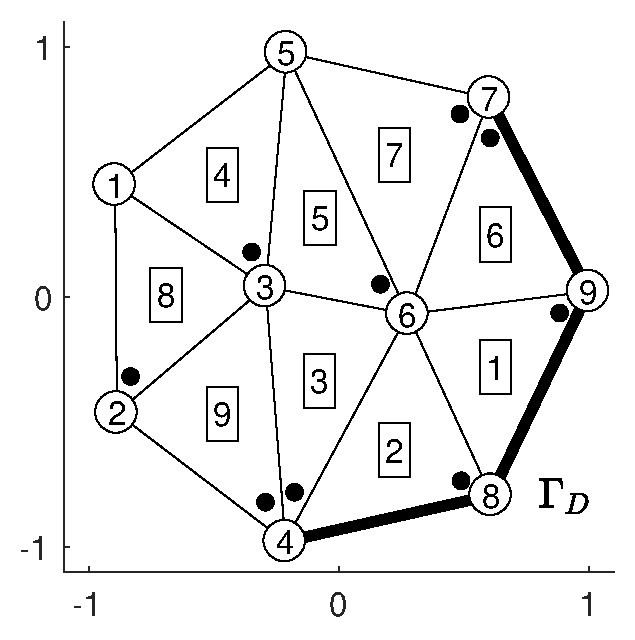
\includegraphics[width=0.35\textwidth]{fe_mesh_p1_bnd}
  \caption{A triangulated domain with a Dirichlet boundary.}
  \label{fig:fe_impl_mesh_p1_bnd}
\end{figure}

\subsection{Inhomogeneous Dirichlet boundary condition}
We now consider an inhomogeneous Dirichlet boundary condition. We recall that we can think of the trial space with an inhomogeneous Dirichlet boundary condition as $\calV^E_h \equiv u^E_h + \calV_h$ where $u^E_h$ is any function in $H^1_h(\Omega)$ such that $u^E_h(z_i) = u^B(z_i)$, $z_i \in \bar \Gamma_D$.  Our finite element problem is as follows: find $\tilde u_h \in \calV_h$ such that
\begin{equation*}
  a(\tilde u_h, v) = \ell(v) - a(u^E_h,v) \quad \forall v \in \calV_h,
\end{equation*}
then set $u_h = u^E_h + \tilde u_h$. For a finite element implementation, it is convenient to choose $u^E_h \in H^1_h(\Omega)$ such that
\begin{equation*}
  u^E_h(z_i) = \begin{cases}
    u^B(z_i), \quad z_i \in \bar \Gamma_D , \\
    0, \quad \text{otherwise}.
  \end{cases}
\end{equation*}
To obtain an equivalent statement for the coefficient $\hat{\tilde u}_h \in \RR^n$, we introduce the following matrices and vectors:
\begin{itemize}
\item $\hat A_h \in \RR^{n \times n}$. The stiffness matrix associated with the  space $\calV_h$ (with the homogeneous Dirichlet boundary condition) as defined in~\eqref{eq:fe_impl_hatAh_dir}.%. The matrix is obtained from $\hat{\bar A}_h \in \RR^{m \times m}$ by removing rows and columns in $S_{\Gamma_D}$ (or, equivalently, by keeping rows and columns in $S_{\calV_h}$).  
\item $\hat f_h \in \RR^n$. The load vector associated with the space $\calV_h$ as defined in~\eqref{eq:fe_impl_hatfh_dir}. % The vector is obtained from $\hat{\bar f}_h \in \RR^m$ by removing the rows in $S_{\Gamma_D}$ (or, equivalently, by keeping rows in $S_{\calV_h}$).
\item $\hat u^E_h \in \RR^{n_{\Gamma_D}}$. The coefficients associated with $u^E_h \in H^1_h(\Omega)$ evaluated on $\Gamma_D$.  We simply set $\hat u^E_h = \{ u^B(z_i) \ | \ z_i \in \bar \Gamma_D \}$, the boundary function $u^B$ evaluated at the Dirichlet nodes.
\item $\hat B_h \in \RR^{n \times n_{\Gamma_D}}$.  The submatrix of the stiffness matrix $\hat{\bar A}_h \in \RR^{m \times m}$ associated with the rows in $S_{\calV_h}$ and the columns in $S_{\Gamma_D}$; i.e., $\hat B_h \{ a(\bar \phi_j, \bar \phi_i) \ | \ i \in S_{\calV_h}, \ j \in S_{\Gamma_D} \}$.
\end{itemize}
Then, the linear-algebraic form of the equation for $\hat{\tilde u}_h \in \RR^n$ is
\begin{equation*}
  \hat A_h \hat{\tilde u}_h = \hat f_h - \hat B_h \hat u^E_h.
\end{equation*}
The solution vector $\hat u_h \in \RR^m$ associated with $u_h \in u^E_h + \calV_h$ is then given by setting for the Dirichlet boundary nodes $\{ \hat u_{h,i} \}_{i \in S_{\Gamma_D}} = \{ u^B(z_i) \}_{i \in S_{\Gamma_D}}$ and for all other nodes $\{ \hat u_{h,i} \}_{i \in S_{\calV_h}} = \hat{\tilde u}_h$.

\section{Efficient implementation by BLAS}
\label{sec:fe_impl_blas}
Before we conclude this lecture, we make a few remarks about an efficient implementation of finite element method on modern computers.  While modern computers can carry out billions of floating point operations per second, modern computers also have deep memory hierarchy and hence not all operations can be carries out as efficiently as others.  One way to achieve a high level of computational utilization on a modern computer is to implement many of the operations as linear algebra operations and to use the basic linear algebra subroutines (BLAS) to carry out those operations.  BLAS routines are optimized for the particular architecture.  There are three different levels of BLAS: BLAS1 deals with vector-vector operations; BLAS2 deals with matrix-vector operations; and BLAS3 deals with matrix-matrix operations. The use of BLAS3 routines, with the most favorable compute-to-memory ratio, is a key to achieve good computational utilization on modern computers.  Many of the operations described in this lecture can be written as BLAS operations.

For instance, suppose we want to evaluate the nodal shape functions at quadrature points of a reference element.  We first write a routine that evaluates monomials: given $n_{\rm pt}$ points described by a matrix $X \in \RR^{n_{\rm pt} \times d}$, evaluate the matrix $\Psi(X) \in \RR^{n_{\rm pt} \times n_s}$, where $(\Psi(X))_{ij}$ is the $j$-th monomial basis function evaluated at the $i$-th point. Using this routine, we can express the Vandermonde matrix as
\begin{equation*}
  V = \Psi(X_{\rm int}) \in \RR^{n_s \times n_s},
\end{equation*}
where $X_{\rm int} \in \RR^{n_s \times d}$ is the set of Lagrange interpolation nodes.  To compute the nodal shape functions at quadrature points $X_{\rm quad} \in \RR^{n_{\rm quad} \times d}$, we appeal to the fact that the Vandermonde matrix is the inverse of the nodal basis coefficient matrix and invoke
\begin{equation*}
  \Phi(X_{\rm quad}) = \Psi(X_{\rm quad}) V^{-1} \in \RR^{n_{\rm quad} \times n_s}.
\end{equation*}
(In the actual implementation, the inverse should never be explicitly computed but its action should be computed through a linear solve.)  This is an efficient and concise way to compute nodal shape functions using matrix operations.

As another example, suppose we now wish to evaluate the mass matrix on the reference element, $\tilde M \equiv \RR^{n_s \times n_s}$ such that
\begin{equation*}
  \tilde M_{ij} = \int_{\tilde K} \phi_i \phi_j dx, \quad \forall i,j = 1,\dots,n_s.
\end{equation*}
If the shape functions are polynomials of degree $p$, then we can exactly evaluate the mass matrix by using a quadrature rule of degree $2p$.
\begin{equation*}
  \tilde M_{ij} = \sum_{q=1}^{n_{\rm quad}} w_q \phi_i(x_q) \phi_j(x_q), \quad \forall i,j = 1,\dots,n_s.
\end{equation*}
Now, we can combine (i) a vector of quadrature weights $w \in \RR^{n_{\rm quad}}$ and (ii) shape functions evaluated at quadrature points $\Phi(X_{\rm quad}) \in \RR^{n_{\rm quad} \times n_s}$ to evaluate the mass matrix as
\begin{equation*}
  \tilde M = \Phi(X_{\rm quad})^T \text{diag}(w) \Phi(X_{\rm quad}).
\end{equation*}
(In \textsc{Matlab}, it is a bit more efficient to replace $\text{diag} w \Phi$ with $\text{bsxfun(@times, } w,\Phi)$.) The mass matrix can then be efficiently computed using a BLAS3 routine.

With some planning, a significant fraction --- or more precisely most computationally intense parts --- of finite element code can be expressed in terms of BLAS routines. The use of BLAS is important for both compiled languages (e.g., C, C++) and interpreted languages (e.g., \textsc{Matlab}, Python).  However, it is arguably more important for the interpreted languages because the efficiency of interpreted languages can be quite limited for simple but computationally intense operations.

\section{Summary}
We summarize key points of this lecture:
\begin{enumerate}
\item Given a polynomial space and a set of nodes, the associated nodal shape functions $\{\tilde \phi_\alpha\}$ can be identified using the Vandermonde method.
\item A finite element is formally defined by (i) a domain, (ii) a finite-dimensional approximation space, and (iii) degrees of freedom used to describe functions in the space.
\item A reference element $\tilde K$ is mapped to a physical element $K$ by using a polynomial geometry mapping $\calG^K$.  The differentiation of the mapping yields the Jacobian $J^K$, from which we compute the determinant of the Jacobian $|J^K|$ and the inverse Jacobian $(J^K)^{-1}$.
\item In $\RR^2$, a reference line segment $\tilde I$ is mapped to a physical facet $F$ by using a polynomial geometry mapping $\calG^F$.  The differentiation of the mapping yields the Jacobian $J^F$, from which we compute the determinant of the Jacobian $J^F$ and the outward-pointing normal vector $n^F$.
\item Physical shape functions on a given element, $\{\phi^K_\alpha\}$, are obtained by mapping the reference shape functions $\{\tilde \phi_\alpha\}$ through the geometry mapping $\calG^K$.
\item On a reference line segment, a $n_q$-point Gauss quadrature rule exactly integrates polynomials of degree up to $2n_q - 1$.  The rule is most efficient in the sense that it requires the fewest number of points to integrate a polynomial of a given degree.
\item Efficient quadrature rules for canonical domains in higher dimensions also exist; however, they are not as well standardized as Gauss quadrature in one dimension.
\item To evaluate the domain-integration terms in local stiffness matrices and load vectors, we (i) map the integration domain from $K$ to $\tilde K$ using the geometry mapping $\calG^K$, (ii) evaluate the integrand, and in particular the physical basis functions $\{\phi_\alpha^K\}$ and their gradients, and (iii) invoke an appropriate quadrature rule.  A similar procedure exists for the boundary-integration terms.
\item Essential boundary conditions are imposed by eliminating shape functions on $\bar \Gamma_D$ from the approximation space. The task translates to the elimination of the rows and columns associated with $\bar \Gamma_D$ from the (global) stiffness matrix and load vector.
\item An efficient finite element solver can be implemented on a modern computer using BLAS routines.
\end{enumerate}

%\section{Efficient implementation by BLAS}

%$\Phi \in \RR^{n_q \times n_s}$
%\begin{equation*}
%  \tilde \Phi_{qi} = \tilde \phi_i(\tilde \xi_q)
%\end{equation*}

%\begin{equation*}
%  \widetilde {\nabla \Phi}_{qij} = \left. \pp{\tilde \phi_i}{\tilde x_j} \right|_{\tilde \xi_q}
%\end{equation*}

%\begin{equation*}
%  \nabla \Phi_{qij} = \left. 
%\end{equation*}




%% \begin{figure}
%%   \centering
%%   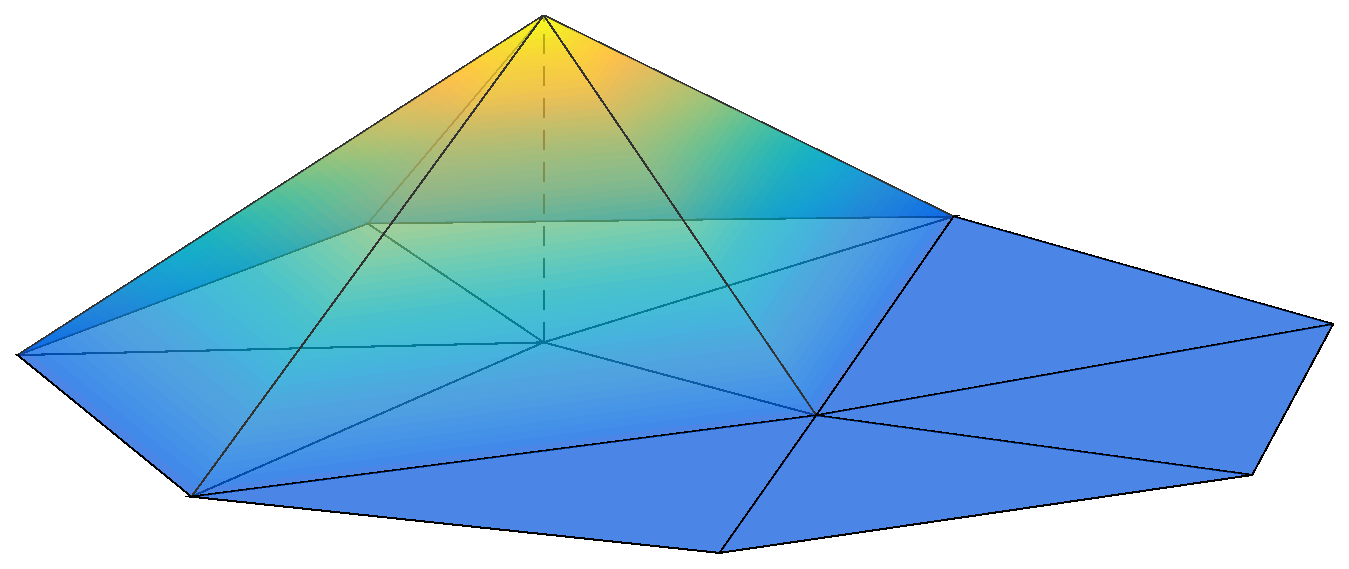
\includegraphics[width=0.48\textwidth]{shape_global_p1}
%% \end{figure}



%% \begin{figure}
%%   \centering
%%   \subfigure[vertex shape function]{
%%     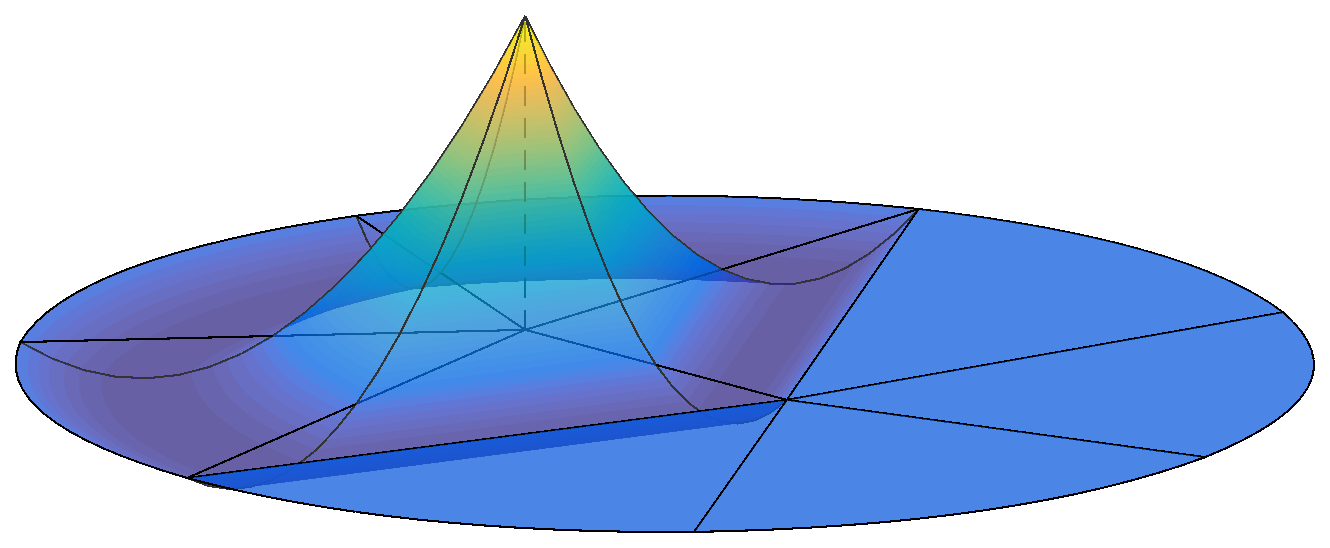
\includegraphics[width=0.48\textwidth]{shape_global_p2_1}
%%   }
%%   \subfigure[edge shape function]{
%%     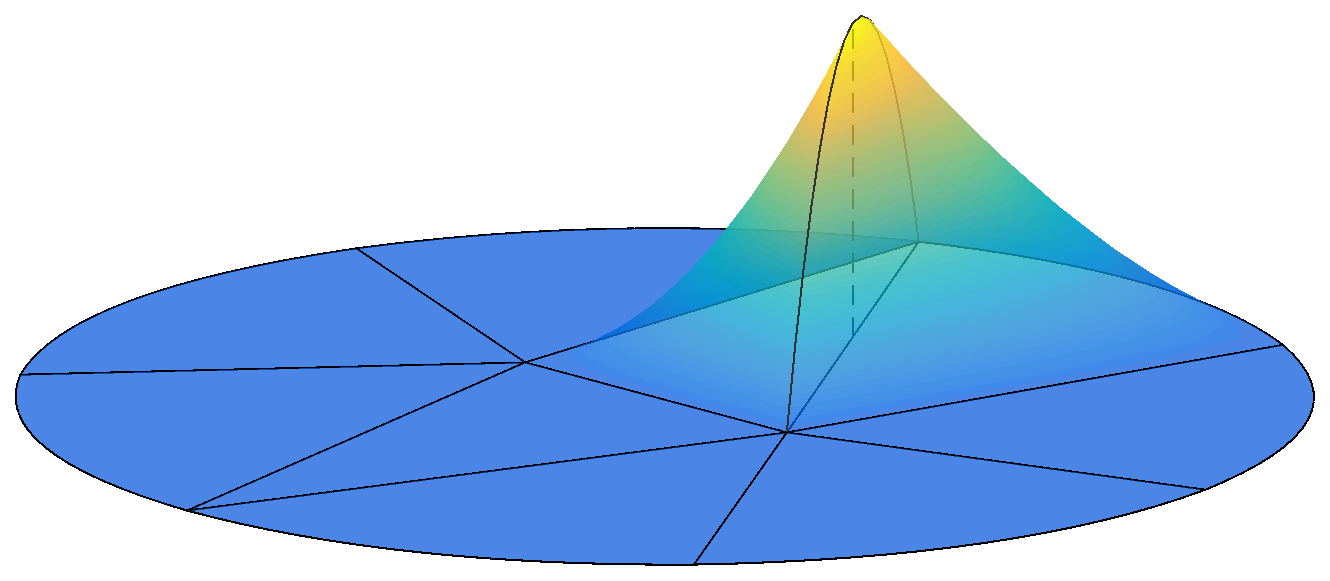
\includegraphics[width=0.48\textwidth]{shape_global_p2_2}
%%   }
%% \end{figure}


%% \begin{figure}
%%  \centering
%%  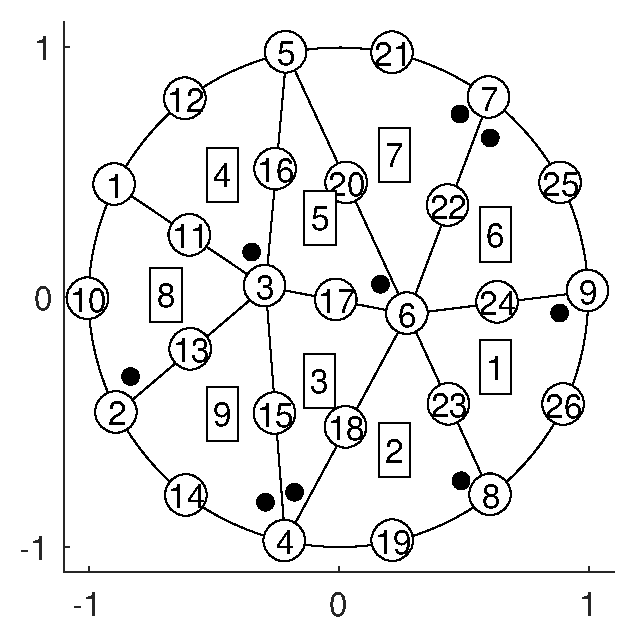
\includegraphics[width=0.4\textwidth]{fe_mesh_p2}
%%  \caption{$p=2$ mesh.}
%%  \label{fig:fe_mesh_p2}
%% \end{figure}
%% \begin{table}
%%   \centering
%%   \subfigure[coordinates]{
%%     \begin{tabular}{c|cc}
%%       node & $x_1$ & $x_2$ \\
%%       \hline
%% $1$ & $-0.89$ & $\hphantom{-}0.45$ \\ 
%% $2$ & $-0.89$ & $-0.46$ \\ 
%% $3$ & $-0.29$ & $\hphantom{-}0.04$ \\ 
%% $4$ & $-0.21$ & $-0.98$ \\ 
%% $5$ & $-0.21$ & $\hphantom{-}0.98$ \\ 
%% $6$ & $\hphantom{-}0.28$ & $-0.07$ \\ 
%% $7$ & $\hphantom{-}0.60$ & $\hphantom{-}0.80$ \\ 
%% $8$ & $\hphantom{-}0.61$ & $-0.79$ \\ 
%% $9$ & $1.00$ & $\hphantom{-}0.02$ \\ 
%% $10$ & $-1.00$ & $-0.01$ \\ 
%% $11$ & $-0.59$ & $\hphantom{-}0.25$ \\ 
%% $12$ & $-0.61$ & $\hphantom{-}0.79$ \\ 
%% $13$ & $-0.59$ & $-0.21$ \\ 
%% $14$ & $-0.61$ & $-0.79$ \\ 
%% $15$ & $-0.25$ & $-0.47$ \\ 
%% $16$ & $-0.25$ & $\hphantom{-}0.51$ \\ 
%% $17$ & $-0.01$ & $-0.01$ \\ 
%% $18$ & $\hphantom{-}0.03$ & $-0.52$ \\ 
%% $19$ & $\hphantom{-}0.22$ & $-0.98$ \\ 
%% $20$ & $\hphantom{-}0.03$ & $\hphantom{-}0.46$ \\ 
%% $21$ & $\hphantom{-}0.22$ & $\hphantom{-}0.98$ \\ 
%% $22$ & $\hphantom{-}0.44$ & $\hphantom{-}0.36$ \\ 
%% $23$ & $\hphantom{-}0.44$ & $-0.43$ \\ 
%% $24$ & $\hphantom{-}0.64$ & $-0.02$ \\ 
%% $25$ & $\hphantom{-}0.89$ & $\hphantom{-}0.46$ \\ 
%% $26$ & $\hphantom{-}0.90$ & $-0.43$ \\   
%%     \end{tabular}
%%   }
%%   \subfigure[connectivity]{
%%     \begin{tabular}{c|cccccc}
%%       element & node 1 & node 2 & node 3 & node 4 & node 5 & node 6\\
%%       \hline
%% $1$ & $9$ & $6$ & $8$ & $23$ & $26$ & $24$ \\ 
%% $2$ & $8$ & $6$ & $4$ & $18$ & $19$ & $23$ \\ 
%% $3$ & $4$ & $6$ & $3$ & $17$ & $15$ & $18$ \\ 
%% $4$ & $3$ & $5$ & $1$ & $12$ & $11$ & $16$ \\ 
%% $5$ & $6$ & $5$ & $3$ & $16$ & $17$ & $20$ \\ 
%% $6$ & $7$ & $6$ & $9$ & $24$ & $25$ & $22$ \\ 
%% $7$ & $7$ & $5$ & $6$ & $20$ & $22$ & $21$ \\ 
%% $8$ & $2$ & $3$ & $1$ & $11$ & $10$ & $13$ \\ 
%% $9$ & $4$ & $3$ & $2$ & $13$ & $14$ & $15$ \\ 
%%     \end{tabular}
%%   }
%%   \caption{Node coordinate and connectivity table for $p=2$ mesh shown in Figure~\ref{fig:fe_mesh_p2}}
%% \end{table}



%i.e., for a piecewise polynomial space $\calV_h$,
%\begin{equation*}
%  \calV_h \subset \calV \quad \Leftrightarrow \quad \calV_h \subset C^0(\overline \Omega) ,
%\end{equation*}
%where  $C^0(\overline \Omega)$ is the space of continuous functions over $\overline \Omega$.

%Given the continuity requirement, we will construct finite element spaces of the form
%\begin{equation}
%  \calV_h \equiv \{ v \in C^0(\overline \Omega) \ | v |_{K_i} \in \PP^p(K_i), \ i = 1,\dots, n_e \};
%  \label{eq:fe_space}
%\end{equation}
%we recall that $\PP^p(K_i)$ is the space of degree $p$ polynomials over $K_i$.





%% \section{Linear Lagrange element on a line segment}
%% \label{sec:fe_lin_line}
%% We first introduce arguably the simplest finite element: linear Lagrange element on a unit line segment $\tilde K$.  Our unit line segment $\tilde K \equiv (\tilde x^1, \tilde x^2)$ is delineated by two endpoints
%% \begin{equation*}
%%   \tilde x^1 = 0 \quad \text{and} \quad \tilde x^2 = 1.
%% \end{equation*}
%% For the linear polynomial space $\PP^1(\tilde K)$ and the interpolation points $\{\tilde x^1, \tilde x^2\}$, a unique set of \emph{Lagrange basis functions} (or \emph{Lagrange shape functions}) is given by
%% \begin{equation*}
%%   \tilde \phi_1(\tilde x) = 1 - \tilde x \quad \text{and} \quad \tilde \phi_2(\tilde x) = \tilde x.
%% \end{equation*}
%% Note that these basis functions satisfy the interpolation condition
%% \begin{equation*}
%%   \phi_i(\tilde x^j) = \delta_{ij}.
%% \end{equation*}
%% Here $\delta_{ij}$ is the \emph{Kronecker delta}: $\delta_{ij} = 1$ for $i = j$ and $\delta_{ij} = 0$ for $i \neq j$.

%% With these basis functions, we can describe any function $v \in \PP^1(\tilde K)$ as
%% \begin{equation*}
%%   v = \sum_{i=1}^{n_s} \tilde v_i \tilde \phi_i
%% \end{equation*}
%% for $\tilde v_i \equiv v(\tilde x^i)$, $i = 1,2$; the values of the function at the end points are the degree of freedom of the finite element.  Similarly, the derivative of the function is given by
%% \begin{equation*}
%%   \pp{v}{\tilde x} = \sum_{i=1}^{n_s} \tilde v_i \pp{\tilde \phi_i}{\tilde x},
%% \end{equation*}
%% where the direct differentiation of the basis functions yields $\pp{\tilde \phi_1}{\tilde x} = -1$ and $\pp{\tilde \phi_2}{\tilde x} = 1$.


%To see the equivalence, we observe that .  Conversely, if a polynomial space is no
%We hence choose
%\begin{equation*}
%  \calV_h \equiv \{ v \in C^0(\overline \Omega) \ | v |_{K_i} \in \PP^p(K_i), \ i = 1,\dots, n_e \};
%\end{equation*}
%





%% Using the linear Lagrange basis functions, we can now represent any function $v$ that is in $\PP^1(\tilde K)$.  Specifically, we may represent $v \in \PP^1(\tilde K)$ in terms of a coefficient vector $\hat v \in \RR^3$ as
%% \begin{equation*}
%%   v(\tilde x) = \sum_{j=1}^{3} \hat v_j  \tilde \phi_j(\tilde x) \quad \forall \tilde x \in \tilde K
%% \end{equation*}
%% for $\hat v_j \equiv v(\tilde x^j)$, $j = 1,2,3$.  We hence have a one-to-one mapping between \emph{any} element in $\PP^1(\tilde K)$ and the associated coefficient vector in $\RR^3$.  For the linear Lagrange basis functions, the coefficients $\hat v \in \RR^3$ is associated with the values of the function at the vertices of the triangle.


%% For a quadratic triangle, the mapping is quadratic and vertices and mid-edge nodes of the reference triangle are mapped to the respective vertices and mid-edge nodes of the physical triangle.

%% Formally, a finite element space is parametrized by the following three properties:
%% \begin{enumerate}
%% \item the triangulation $\calT_h$ of $\Omega$;
%% \item the type of functions that constitutes the space (e.g., piecewise linear polynomial);
%% \item the degrees of freedom used to describe functions in the space.
%% \end{enumerate}
%% The first two are apparent from the definition of the finite element space~\eqref{eq:fe_space}.  The last property determines how a function $v \in \calV_h$ is represented on a computer.  Specifically, given a $N$-dimensional function space $\calV_h$, we assign $N$ degrees of --- by choosing $N$ basis functions --- such that the a function $v \in \calV_h$ can be uniquely described by $N$ real numbers.  We will clarify this third property in Section~\ref{sec:fe_map}.


%% \section{Bilinear Lagrange element on a quadrilateral}
%% We now consider arguably the simplest basis function on quadrilaterals: bilinear Lagrange basis on a reference quadrilateral.  Our reference quadrilateral is a unit square that is delineated by vertices
%% \begin{equation*}
%%   x^1 = (0,0), \quad x^2 = (1,0), \quad x^3 = (0,1), \quad \text{and} \quad x^4 = (1,1).
%% \end{equation*}
%% In two dimensions, any bilinear function can be expressed as a linear combination of monomial basis $\{ 1, x_1, x_2, x_1 x_2 \}$, which, unlike the triangular case, includes the cross term. Our interpolation points are the four vertices of the quadrilateral $\{ x^1, x^2, x^3, x^4 \}$.  Our shape functions are given by 
%% \begin{equation}
%%   \phi_i(x) = a_1^i + a_2^i x_1 + a_3^i x_2 + a_4^i x_1 x_2, \quad i = 1,\dots,4,
%%   \label{eq:fe_lin_quad_rep}
%% \end{equation}
%% where the coefficients satisfy
%% \begin{equation*}
%%   \bmat{cccc}
%%   1 & x_1^1 & x_2^1 & x_1^1 x_2^1 \\
%%   1 & x_1^2 & x_2^2 & x_1^2 x_2^2 \\
%%   1 & x_1^3 & x_2^3 & x_1^3 x_2^3 \\
%%   1 & x_1^4 & x_2^4 & x_1^4 x_2^4 \\
%%   \emat
%%   \bmat{cccc}
%%   a_1^1 & a_1^2 & a_1^3 & a_1^4 \\
%%   a_2^1 & a_2^2 & a_2^3 & a_2^4 \\
%%   a_3^1 & a_3^2 & a_3^3 & a_3^4 \\
%%   a_4^1 & a_4^2 & a_4^3 & a_4^4 \\
%%   \emat
%%   =
%%   \bmat{cccc}
%%   1 & 0 & 0 & 0 \\
%%   0 & 1 & 0 & 0 \\
%%   0 & 0 & 1 & 0 \\
%%   0 & 0 & 0 & 1
%%   \emat.
%% \end{equation*}
%% Once we find the coefficients, we can evaluate the value of the shape function at any point in the quadrilateral by evaluating~\eqref{eq:fe_lin_quad_rep}. We can also differentiate~\eqref{eq:fe_lin_quad_rep} to obtain gradient of the shape functions:
%% \begin{equation*}
%%   \pp{\phi_i}{x_1}(x) = a_2^i + a_4^ix_2
%%   \quad \text{and} \quad
%%   \pp{\phi_i}{x_2}(x) = a_3^i + a_4^ix_1, \quad i = 1,\dots,4.
%% \end{equation*}
%% Unlike the linear shape functions for triangles, the gradient of the \emph{bi}linear shape functions for quadrilateral depends on the evaluation point.


%% Formally, a finite element is defined by a triplet $(K,\calP,\Sigma)$ where
%% \begin{itemize}
%% \item[(i)] $K$ defines the domain
%% \item[(ii)] $\calP$ defines the (finite-dimensional) linear space of functions over $K$
%% \item[(iii)] $\Sigma$ defines the degrees of freedom such that a function $v \in \calP$ is uniquely determined.
%% \end{itemize}
%% For instance, for the linear Lagrange element in Section~\ref{sec:fe_lin_tri} chooses (i) the triangle as the domain $K$, (ii) space of linear functions $\PP^1(K)$ as the function space $\calP$, and (iii) the values of the function at the vertices of the triangle as the degree of freedom $\Sigma$. 

%% In general, a Lagrange basis is uniquely determined by (i) the degree of polyno
